\documentclass[11pt]{scrartcl}
\usepackage{color}
\usepackage{enumitem}
\setlist[itemize,2]{label=\textbullet}
\usepackage{geometry}
\geometry{a4paper, top=25mm, left=20mm, right=20mm, bottom=40mm, headsep=10mm, footskip=5mm}
\usepackage{ucs}
\usepackage[utf8x]{inputenc}
%\usepackage{german}
\usepackage{soul}
\usepackage{amsmath,amssymb,amstext}
\usepackage{graphicx}
\usepackage[automark]{scrpage2}
\usepackage{subcaption}
%\usepackage{caption}
%\usepackage{subfigure}
%\usepackage{subfig}

\usepackage{algpseudocode,algorithm,algorithmicx}
\newcommand*\DNA{\textsc{dna}}

\newcommand*\Let[2]{\State #1 $\gets$ #2}
\algrenewcommand\algorithmicrequire{\textbf{Precondition:}}
\algrenewcommand\algorithmicensure{\textbf{Postcondition:}}

\usepackage[ngerman]{babel} 
\usepackage{xspace}
\usepackage{hyperref}
%\RequirePackage[ngerman=ngerman-x-latest]{hyphsubst}
\newcommand{\Gu}{\glqq{}}		%Gänsefüßchen unten
\newcommand{\Go}{\grqq\xspace} 
\newcommand{\red}{\textcolor{red}}
\newcommand{\ita}{\item[$\rightarrow$]}
\DeclareSymbolFont{matha}{OML}{txmi}{m}{it}% txfonts
\DeclareMathSymbol{\varv}{\mathord}{matha}{118}
\renewcommand*\labelitemii{-}
%\newcommand{\tightemize}{\vspace{-2mm}\begin{itemize}\setlength\itemsep{0em}}
\pagestyle{scrheadings}
\pagenumbering{arabic}	        %Gänsefüßchen oben
 \addtolength{\textheight}{25mm}
%\title{Lernende und Planende Roboter}
%\author{Sophie v. Schmettow}
%\date{\today{} in Karlsruhe}

\begin{document}

%----------------------------------------------------------------------------------------
%	TITLE PAGE
%----------------------------------------------------------------------------------------
\begin{titlepage}

\begin{center}


% Upper part of the page

\includegraphics[width=0.4\textwidth]{Logo_KIT.png}\\[1cm]    



\textsc{\Large Zusammenfassung}\\[0.5cm]


% Title
{ \huge \bfseries Lernende und Planende Roboter}\\[0.4cm]
{ \large \bfseries (Robotik II)}
\bigskip

% Author and supervisor

Sophie \textsc{v. Schmettow}
SoSe 15\\



\vfill

% Bottom of the page
{\large \today{} in Karlsruhe} 

\end{center}


\end{titlepage}

%----------------------------------------------------------------------------------------
%	ARTICLE CONTENTS
%----------------------------------------------------------------------------------------

\tableofcontents
\newpage

%----------------------------------------------------------------------------------------
%	UTILS
%----------------------------------------------------------------------------------------

%\begin{figure*}[ht]\centering % Using \begin{figure*} makes the figure take up the entire width of the page
%\includegraphics[width=\linewidth]{view}
%\caption{Wide Picture}
%\label{fig:view}
%\end{figure*}



%\begin{equation}
%\cos^3 \theta =\frac{1}{4}\cos\theta+\frac{3}{4}\cos 3\theta
%\label{eq:refname2}
%\end{equation}



%\begin{enumerate}[noitemsep] % [noitemsep] removes whitespace between the items for a compact look
%\item First item in a list
%\item Second item in a list
%\item Third item in a list
%\end{enumerate}



%\begin{figure}[ht]\centering
%\includegraphics[width=\linewidth]{results}
%\caption{In-text Picture}
%\label{fig:results}
%\end{figure}

%Reference to Figure \ref{fig:results}.


%\begin{table}[hbt]
%\caption{Table of Grades}
%\centering
%\begin{tabular}{llr}
%\toprule
%\multicolumn{2}{c}{Name} \\
%\cmidrule(r){1-2}
%First name & Last Name & Grade \\
%\midrule
%John & Doe & $7.5$ \\
%Richard & Miles & $2$ \\
%\bottomrule
%\end{tabular}
%\label{tab:label}
%\end{table}



%\begin{description}
%\item[Word] Definition
%\item[Concept] Explanation
%\item[Idea] Text
%\end{description}

%----------------------------------------------------------------------------------------
%	ARTICLE CONTENTS
%----------------------------------------------------------------------------------------

\section*{Disclaimer}
Dieses Dokument wurde im Rahmen des Master-Studiums
für das Modul Autonome Robotik erstellt. Es stellt eine 
Zusammenfassung dar und dient zur Vorbereitung auf die
mündliche Prüfung. Neben den Materialien der Vorlesung,
fließen auch weitere Quellen ein, um den behandelten Stoff
auszuarbeiten. Auf den Verweis von Quellen wird verzichtet,
da die Erstellung keinerlei wissenschaftlichen Zweck verfolgt
und nur für den privaten Gebrauch bestimmt ist.

\section{Einführung und Grundlagen} %(1. VL)
\subsection{Klassifizierung der Verfahren zur Roboterprogrammierung}
\begin{figure}[ht]\centering 
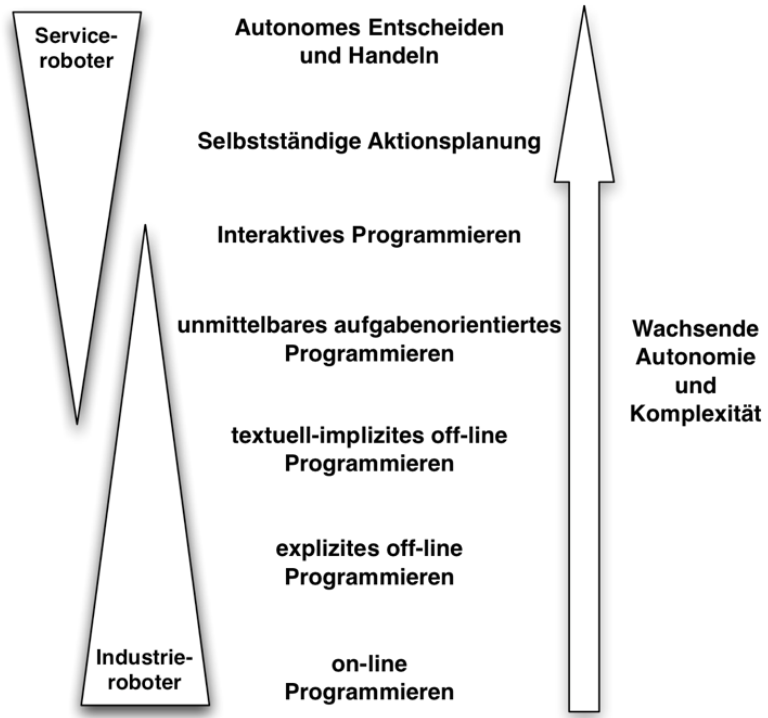
\includegraphics[width=0.5\linewidth]{figures/ch01_ueberblick.png}
\caption{Überblick}
\label{fig:ch01_komp}
\end{figure}
Kriterien:
\begin{itemize}
\item[1.] \textbf{Programmierort:} On-line (prozessnah, am Roboter) vs. Off-line (prozessfern, ohne Roboter)
\item[2.] \textbf{Art der Programmierung:} Direkte vs. indirekte (textuelle oder graphische/gemischte) Programmierung, hybride Verfahren
\item[3.] \textbf{Abstraktionsgrad der Programmierung:} Explizite/bewegungs- bzw. roboterorientierte vs. implizite/aufgabenorientierte Programmierung
\end{itemize}
\begin{figure}[ht]\centering 
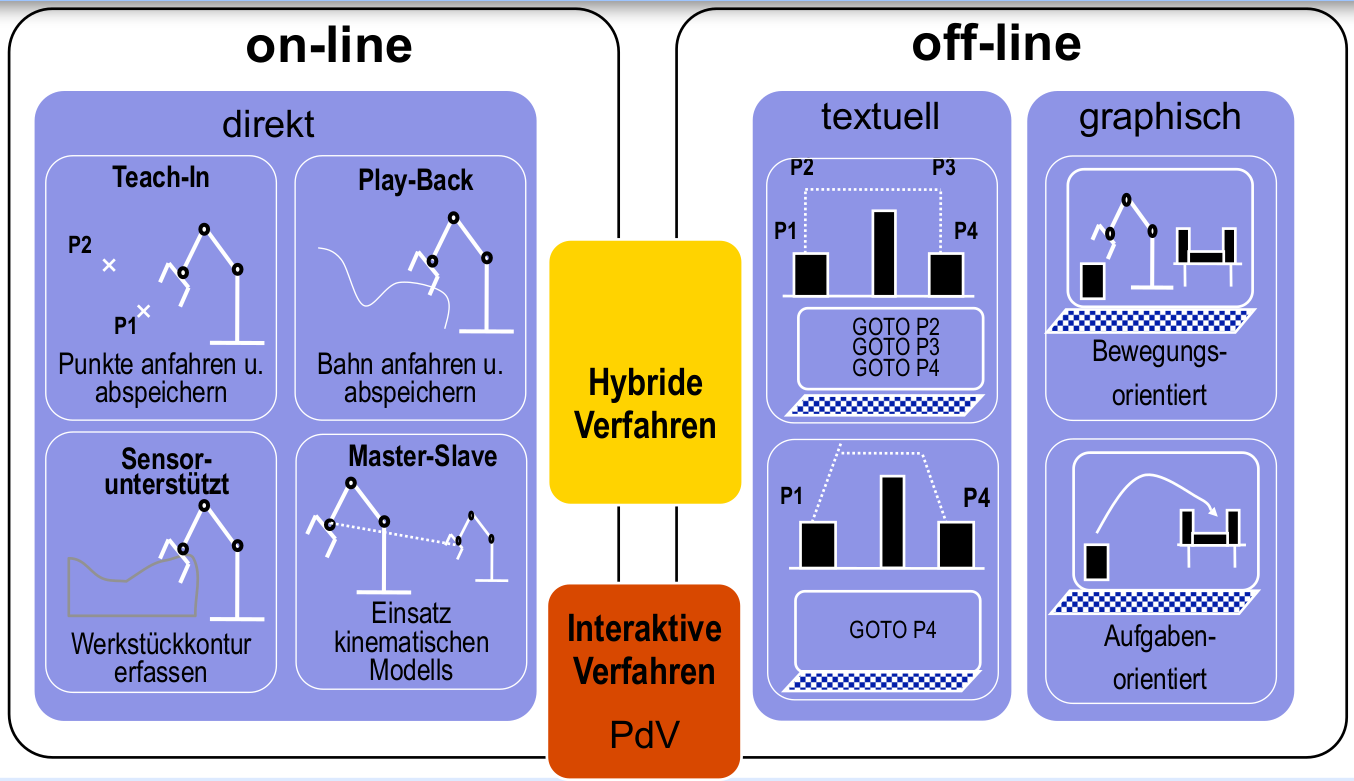
\includegraphics[width=\linewidth]{figures/ch01_schema.png}
\caption{Schema}
\label{fig:ch01_schema}
\end{figure}
\subsection{Arten der Programmierung}
\subsubsection{Direkte/Prozessnahe Programmierung}
\begin{itemize}
\item \textbf{Einstellen des Roboters:} Ältestes Programmierverfahren.
Der Bewegungsbereich jedes Gelenks wird durch Stopper eingeschränkt.
Die Bewegungen erfolgen für jedes Gelenk einzeln bis zum Anschlag.
Zuordnung zwischen Anfahrpunkten zu Stopper kann mit Codiermatritzen erfolgen.
(sogenannter \glqq Bang-Bang-Robot\grqq)\\
Nachteil: sehr kleine Menge von Anfahrpunkten.
\item \textbf{Teach-In Programmierung:} Anfahren markanter Punkte der Bahn mit manueller Steuerung
(Teach Box, Teach Panel, weitere: Spacemouse, Teach-Kugel)\\
Funktionalität einer Teach Box:
\begin{itemize}
\item Einzelbewegung der Gelenke
\item Bewegung des Effektors in 6 Freiheitsgraden
\item Punkte anfahren u. abspeichern
\item Speichern / Löschen von Anfahrpunkten
\item Eingabe von Geschwindigkeiten
\item Eingabe von Befehlen zur Bedienung des Greifers
\item Starten / Stoppen ganzer Programme
\end{itemize}
Vorgehensweise beim Teach-In:
\begin{itemize}
\item Anfahren markanter Punkte der Bahn (= Folge von Zwischenpunkten)
\item Speichern der Gelenkwerte
\item Ergänzung der gespeicherten Werte
um Parameter wie Geschwindigkeit, Beschleunigung usw.
\item Anwendung: in der Fertigungsindustrie (Punktschweißen, Nieten), Handhabungsaufgaben (Pakete vom Fließband nehmen)
\end{itemize}
\item \textbf{Play-Back- (manuelle) Programmierung:}
\begin{itemize}
\item Einstellung des Roboters auf Zero-Force-Control
(Roboter kann durch den Bediener bewegt werden)
\item Abfahren der gewünschten Bahn
\item Speichern der Gelenkwerte: automatisch (definierte Abtastfrequenz) oder manuell (durch Tastendruck)
\item Anwendung: mathematisch schwer beschreibbare Bewegungsabläufe, Integrierung der handwerklichen Erfahrung, typischerweise für Lackieren oder Kleben eingesetzt
\end{itemize}
\begin{table}[hbt]
\centering
\begin{tabular}{|p{13cm}|}
\hline
Nachteile\\
\hline
\vspace{-5mm}
\begin{itemize}
\setlength\itemsep{0em}
\item[-] schwere Roboter schwierig zu bewegen
\item[-] wenig Platz in engen Fertigungszellen für Bediener, dadurch Sicherheitsrisiko
\item[-] hoher Speicherbedarf (bei hoher Abtastrate)
\item[-] schlechte Korrekturmöglichkeiten
\end{itemize}\\
\hline
\end{tabular}
\caption{Nachteile der Play-Back-Programmierung}
\label{tab:PBprog}
\end{table}
\newpage
\item \textbf{Master-Slave-Programmierung:}
\begin{itemize}
\item Bediener führt einen kleinen, leicht bewegbaren Master
Roboter (entspricht einem kinematischen Modell des
Slave-Roboters)
\item Bewegung wird auf den Slave-Roboter übertragen
\item Bewegungen werden synchron ausgeführt
\item Slave-Roboter wirkt als Kraftverstärker
\item Anwendung: Handhabung großer Lasten bzw. großer Roboter
\end{itemize}
\begin{table}[hbt]
\centering
\begin{tabular}{|p{6.5cm}|p{6.5cm}|}
\hline
Vorteile & Nachteile\\
\hline
\vspace{-5mm}
\begin{itemize}
\setlength\itemsep{0em}
\item[+] Möglichkeit, auch schwerste Roboter zu programmieren
\end{itemize}
 &
 \vspace{-5mm}
\begin{itemize}
\setlength\itemsep{0em}
\item[-] teuer, da zwei Roboter benötigt werden
\end{itemize}\\
\hline
\end{tabular}
\caption{Zusammenfassung Master-Slave-Programmierung}
\label{tab:MSprog}
\end{table}
\item \textbf{Sensorunterstützte Programmierung:}\\
Manuell
\begin{itemize}
\item Bediener führt Programmiergriffel (Leuchtstift, Laserstift) entlang der
abzufahrenden Bahn
\item Erfassung der Bewegung durch externe Sensoren (zB. Kameras,
Laserscanner)
\item Berechnung der inversen Kinematik
\end{itemize}
Automatisch
\begin{itemize}
\item Vorgabe des Start- und Zielpunktes
\item Sensorische Ertastung der Sollkontur (zB. über Kraft-Momenten-Sensor)
\end{itemize}
Anwendung: Abspeichern der Bahn als Folge der Gelenkwinkel
Schleifen, Entgraten von Werkstücken	
\end{itemize}
\begin{table}[hbt]
\centering
\begin{tabular}{|p{7.5cm}|p{7.5cm}|}
\hline
Vorteile & Nachteile\\
\hline
\vspace{-5mm}
\begin{itemize}
\setlength\itemsep{0em}
\item[+] schnell bei einfachen Trajektorien
\item[+] sofort anwendbar
\item[+] geringe Fehleranfälligkeit
\item[+] Bediener benötigt keine Programmierkenntnisse
\item[+] kein Modell der Umwelt erforderlich
\end{itemize}
 &
 \vspace{-5mm}
\begin{itemize}
\setlength\itemsep{0em}
\item[-] hoher Aufwand bei komplexen Trajektorien
\item[-] nur mit und am Roboter möglich
\item[-] spezifisch für einen Robotertyp
\item[-] Verletzungsgefahr durch Roboter
\end{itemize}\\
\hline
\end{tabular}
\caption{Zusammenfassung Direkte Programmierung}
\label{tab:dirprog}
\end{table}
\subsubsection{Textuelle Verfahren}
Erstellung von Robotersteuerprogrammen erfolgt mittels erweiterter,
höherer Programmiersprachen (PasRo, Val, etc.)
\\ \\
\textbf{Sprache:} (DIN 66025)
\begin{itemize}
\item Programm = Menge numerierter Sätze\\
z.B. \glqq N70 G00 X20 Z12\grqq{} entspricht Werkzeug im Eilgang (G00) an Position X=20 Z=12 bewegen. (N = Satznummer)
\item Sprachen:
\begin{itemize}
\item APT (Automatically Programmed Tools), 1961 MIT
\item EXAPT (Extended Subset of APT), 1966 Aachen
\end{itemize}
\end{itemize}

\begin{table}[!h]
\centering
\begin{tabular}{|p{7.5cm}|p{7.5cm}|}
\hline
Vorteile & Nachteile\\
\hline
\vspace{-5mm}
\begin{itemize}
\setlength\itemsep{0em}
\item[+] Programmierung kann unabhängig vom Roboter erfolgen
\item[+] strukturierte, übersichtliche Programmierlogik
\item[+] Erstellung komplexer Programme (Einbezug von Wissensbasis,
Weltmodell, Auswertung von Sensoren)
\end{itemize}
 &
 \vspace{-5mm}
\begin{itemize}
\setlength\itemsep{0em}
\item[-] Bediener benötigt Programmierkenntnisse
\item[-] keine / schlechte Korrekturmöglichkeiten
\end{itemize}\\
\hline
\end{tabular}
\caption{Zusammenfassung Textuelle Verfahren}
\label{tab:textprog}
\end{table}
\subsubsection{Graphische/Gemischte Verfahren}
\begin{itemize}
\item Graphische Darstellung von Kontrollstrukturen (if/else, Schleifen,
Marken...)
\item Kopplung mit Visualisierungs-Tool und Simulations-Tool (z.B. RobCAD)
\item  Trajektorien durch Interpolation aus Stützpunkten, Freihandzeichnen,
analytisch
\item Operationen Icon- oder Menu-gesteuert
\item Simple graphische Programmierung, z.B. Lego Mindstorms:
Leicht verständliche, ikonische Programmierung aber beschränkte Möglichkeiten
\item Graphische Programmierung basierend auf sensorieller Erfassung der
Benutzervorführung:\\ Simulation der Roboterprogramme
\end{itemize}
\begin{table}[hbt]
\centering
\begin{tabular}{|p{7.5cm}|p{7.5cm}|}
\hline
Vorteile & Nachteile\\
\hline
\vspace{-5mm}
\begin{itemize}
\setlength\itemsep{0em}
\item[+] Programmierer benötigt weniger Programmierkenntnisse
\item[+] einfache Programmierung, leichte Fehlererkennung
\item[+] schnelles Erstellen komplexer Programme (rapid prototyping)
\end{itemize}
 &
 \vspace{-5mm}
\begin{itemize}
\setlength\itemsep{0em}
\item[-] sensorielle Benutzererfassung noch zu ungenau
\item[-] Leistungsfähige Hardware für Signalanalyse, Modellierung, ...
\item[-] Komplexe Modelle benötigt
\item[-] 2D-Sicht des Anwenders
\end{itemize}\\
\hline
\end{tabular}
\caption{Zusammenfassung Graphische Verfahren}
\label{tab:textprog}
\end{table}
\newpage
\subsection{Abstraktionsgrad der Programmierung}
\subsubsection{Explizite/Roboterorientierte Programmierung}
\textcolor{red}{\glqq Wie ist es zu tun?\grqq} \\
Bewegungen und Greiferbefehle sind direkt in eine Programmiersprache eingebunden.\\
Das Aufgabenmodell ist gegeben durch Anfangs- und Endzustand (z.B. Relationale Darstellung). Ein Beispiel ist in \autoref{cranfield} dargestellt.\\
\begin{figure}[h!]\centering 
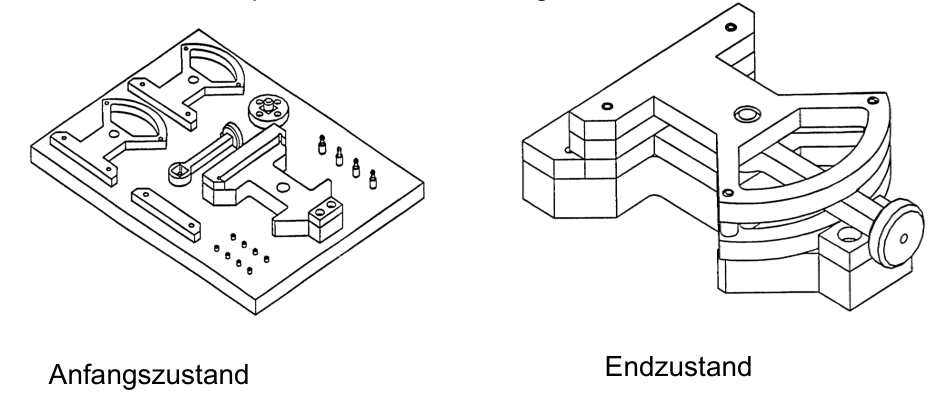
\includegraphics[width=0.7\linewidth]{figures/ch01_cranfield.png}
\caption{Der Cranfield-Montage-Benchmark}
\label{cranfield}
\end{figure}\\
\paragraph{Anwender $\rightarrow$ Roboter}
Jedes Robotersystem besitzt eine roboterabhängige Steuerungsebene, welche folgende Eigenschaften kapselt:
\begin{itemize}
\item Ansteuerung der Hardware (sowohl interne als auch externe)
\item Bewegungsaktionen
\item Lokale Modelle
\item Elementare Operationen (erfordern evtl. Echtzeitregelung)
\end{itemize}
\begin{figure}[h!]\centering 
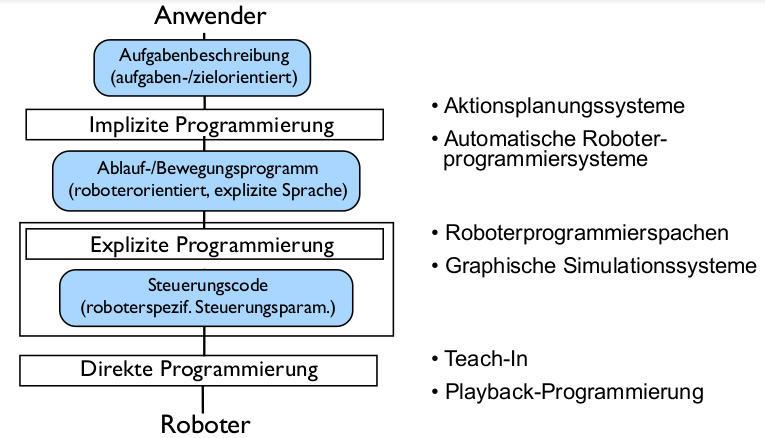
\includegraphics[width=0.7\linewidth]{figures/ch01_einordnung.png}
\caption{Einordnung roboterorientierte Programmierung}
\label{einord}
\end{figure}
\paragraph{Anforderungen an die roboterorientierte Programmierung}
\begin{itemize}
\item Positions-, Geschwindigkeitsregelung der aktiven Komponenten (z.B. Gelenke, Räder)
\item Auslesen und Parametrieren der internen und externen Sensorik
\item Koordinatentransformationen, direkte und inverse Kinematik
\item Sensorabhängige Regelung
\item Verfahren auf Trajektorien
\item Generierung und Zusammensetzen von Trajektorien zu komplexen Bewegungen
\item Verkettung komplexer Bewegungen zu Elementaroperationen
\end{itemize}
\paragraph{Komponenten der roboterorientierten Programmierung}
\autoref{zykl}\\
\begin{figure}[h!]\centering 
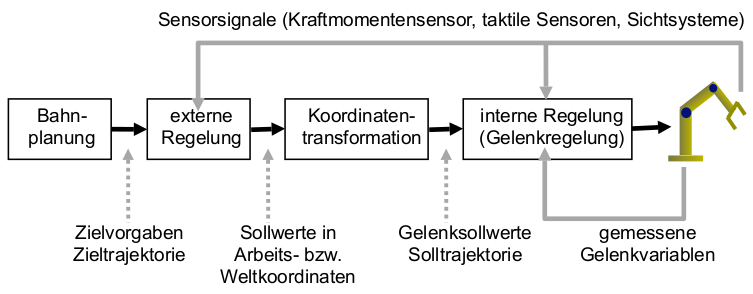
\includegraphics[width=0.7\linewidth]{figures/ch01_zykl.png}
\caption{Regelungszyklus eines Roboters}
\label{zykl}
\end{figure}\\
\paragraph{Sprachelemente von Roboterprogrammiersprachen}
\begin{itemize}
\item Befehle für:
\begin{itemize}
\item Bewegung eines oder mehrerer Roboter
\item Betrieb von Greifern / Werkzeugen
\item Ein-/Ausgabe von Daten / Signalen über Schnittstellen
\item Externe Sensoren
\item Zur Synchronisation / Kommunikation zwischen Prozessen
\item Parallelverarbeitung
\item Zur logischen Verkettung von Koordinatensystemen
\end{itemize}
\item Anweisungen zur Ablaufsteuerung
\item Definition generischer Operationen (zB. Armbewegung + Griff $\rightarrow$ ein Operator)
\end{itemize}
\paragraph{Bewegungsanweisungen}
\begin{itemize}
\item Bewegungen im Gelenkwinkelraum:
\begin{itemize}
\item Bewege alle Gelenke mit max. Geschwindigkeit
\item Regelung der Geschwindigkeiten mit gleichzeitiger Beendigung der Bewegung aller Gelenke
\end{itemize}
\item Kartesische Bewegungen (Stellung des TCPs)
\begin{itemize}
\item Erfordert inverse Kinematik
\item Nutzung von Frames, z.B. relativ zu einem Objekt
\end{itemize}
\item Geometriebezogene Bahndefinition
\end{itemize}
\begin{table}[hbt]
\centering
\begin{tabular}{|p{7.5cm}|p{7.5cm}|}
\hline
Vorteile & Nachteile\\
\hline
\vspace{-5mm}
\begin{itemize}
\setlength\itemsep{0em}
\item[+] Hohe Einstellgenauigkeit der Position
\item[+] Hohe Wiederholgenauigkeit
\item[+] eindeutige Roboterkonfiguration
\item[+] keine inverse Kinematik erforderlich
\end{itemize}
 &
 \vspace{-5mm}
\begin{itemize}
\setlength\itemsep{0em}
\item[-] Abhängigkeit von Robotertyp
\item[-] kein Bezug der Gelenkwinkel zur Objektlage
\end{itemize}\\
\hline
\end{tabular}
\caption{Bewegungen im Gelenkwinkelraum}
\label{tab:bew}
\end{table}
\paragraph{Sprachelemente -- Semantik von Greiferbefehlen}
\begin{itemize}
\item Verschiedene Greifertypen: evtl. mit taktiler und/oder Kraftsensorik
\item Backengreifer: Industrie, Forschung (z.B. 3-Finger-Hand)
\end{itemize}
Mit zunehmender Abstraktion:
\begin{enumerate}
\item Steuerung im Gelenkwinkel-Raum
\begin{itemize}
\item Anzahl der Freiheitsgrade bestimmt Anzahl der Parameter (Backengreifer: 1, menschl. Hand: 22)
\item Wenig Kapselungs-Aufwand (keine inverse Kinematik nötig) 
\item Hand-abhängig
\item Kein Bezug zwischen Fingerstellung und Handstellung
\end{itemize}
\item Steuerung im kartesischen/ zylindrischen/... Raum
\begin{itemize}
\item Parameter: Position/Orientierung jedes Fingers/ jeder Fingerspitze
\item Inverse Kinematik nötig
\item Berechnung aus Greif-/ Bewegungsplanung oder aus menschlicher Vorführung
\item Mögliche Konfigurationen (Konfigurationsraum) handabhängig
\end{itemize}
\item Semantische Steuerung
\begin{itemize}
\item Parameter: Griff-Form, zu greifendes Objekt, Objektgröße, Objektform, ...
\item Mapping auf Roboterhand nötig
\item Übertragbar auf andere Roboterhände (mögliche Griffe handabhängig)
\item Griff-Form vom Menschen lernbar
\end{itemize}
\end{enumerate}
\paragraph{Zusammenfassung -- Explizite Programmierung} Nur in Verbindung mit (abstrakten) Programmiersprachen
\begin{table}[hbt]
\centering
\begin{tabular}{|p{7.5cm}|p{7.5cm}|}
\hline
Vorteile & Nachteile\\
\hline
\vspace{-5mm}
\begin{itemize}
\setlength\itemsep{0em}
\item[+] beliebig komplexe Bahnen
\item[+] Anbindung von Sensoren
\item[+] reaktive Planung
\end{itemize}
 &
 \vspace{-5mm}
\begin{itemize}
\setlength\itemsep{0em}
\item[-] Keine standardisierte Programmiersprache
\item[-] Kenntnis der Programmiersprache
\end{itemize}\\
\hline
\end{tabular}
\caption{Bewegungen im Gelenkwinkelraum}
\label{tab:bew}
\end{table}
\subsubsection{Implizite/Aufgabenorientierte Programmierung}
\textcolor{red}{\glqq Was ist zu tun?\grqq} \\
Die Aufgabe, die der Roboter durchführen soll, wird beschrieben, z.B. in Form von Zuständen.
\begin{itemize}
\item Abstrakte Form der Programmierung erfolgt in den Phasen\\
1. Modellierung der Umwelt\\
2. Spezifikation der Aufgaben\\
3. Erzeugung der Roboterprogramme
\item u. U. erfolgt vor der Ausführung eine Überprüfung des
Roboterprogramms (Simulation)
\item Beispiel: Einschenken unter Berücksichtigung von Hindernissen
\item Details im kommenden Kapitel
\end{itemize}

\section{Aufgabenorientierte Programmierung} %(2. VL)
\subsection{Umweltmodellierung}
\begin{figure}[ht]\centering 
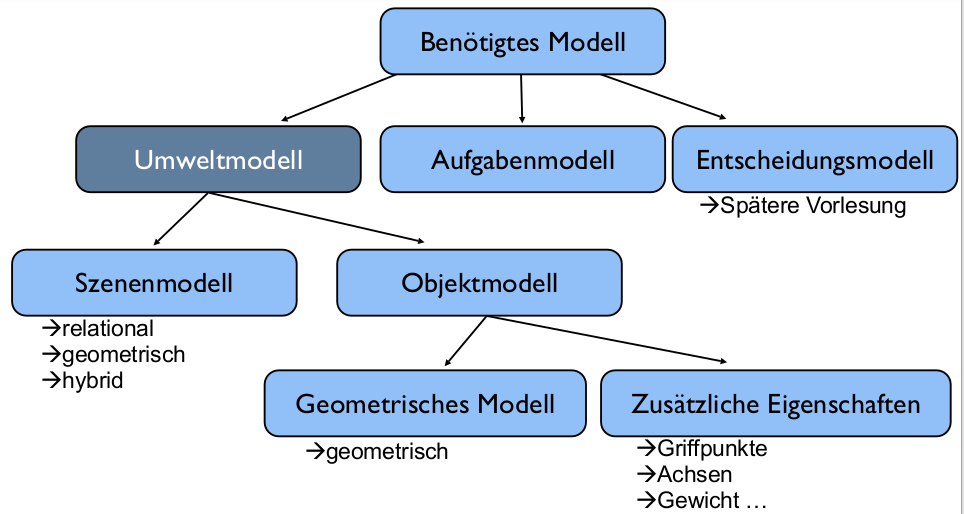
\includegraphics[width=0.6\linewidth]{figures/ch02_umweltmodell.png}
\caption{Umweltmodell}
\label{fig:ch02_um}
\end{figure}

%Keine Umlaute in labels!!!
\subsubsection{Objektmodell}
Die geometrische Beschreibung von Objekten beinhaltet:
\begin{itemize}
\setlength\itemsep{0em}
\item graphische Darstellung
\item Kollisionsberechnungen, Kontaktberechnung in Griffplanung, ...
\item physikalisch-dynamische Simulation der Effekte von Handlungen auf die Umwelt
\item geometriebezogene Bewegungsplanung
\end{itemize}
Es gibt drei Ansätze zur geometrischen Modellierung (\autoref{fig:obrepr}): 
\begin{enumerate}
\item Kantenmodelle
\item Flächenmodelle
\item Volumenmodelle
\end{enumerate}
\begin{figure}[h!]
	\centering
	\begin{subfigure}{.25\textwidth}
		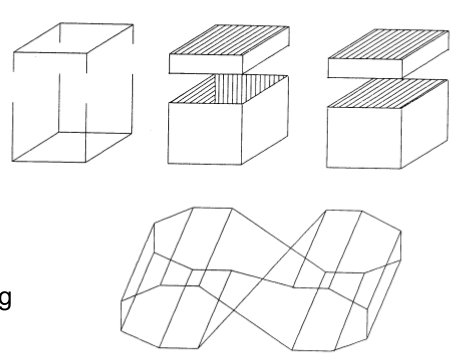
\includegraphics[width=\textwidth]{figures/ch02_kanten.png}
		\caption{}
	\end{subfigure}
	\begin{subfigure}{.25\textwidth}
		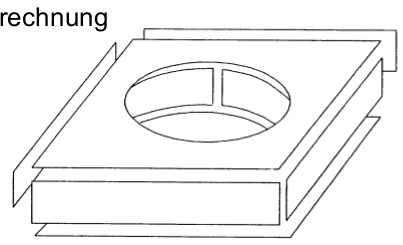
\includegraphics[width=\textwidth]{figures/ch02_flaechen.png}
		\caption{}
	\end{subfigure}
	\begin{subfigure}{.25\textwidth}
		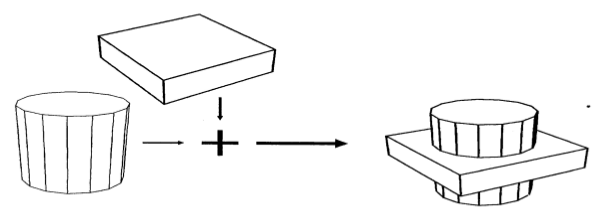
\includegraphics[width=\textwidth]{figures/ch02_volumen.png}
		\caption{}
	\end{subfigure}
	\caption{Objektrepr\"{a}entation}
	\label{fig:obrepr}
\end{figure}
\paragraph*{Kanten}
Nur die Kanten werden gespeichert, d.h. Punkte und Verbindungen (Gerade, Polygonzug, Bezierkurve, ... ).
\begin{table}[hbt]
\centering
\begin{tabular}{|p{6.5cm}|p{6.5cm}|}
\hline
Vorteile & Nachteile\\
\hline
\vspace{-5mm}
\begin{itemize}
\setlength\itemsep{0em}
\item[+] einfache Daten
\item[+] wenige Daten
\end{itemize}
 &
 \vspace{-5mm}
\begin{itemize}
\setlength\itemsep{0em}
\item[-] Mehrdeutigkeiten
\item[-] hoher Eingabeaufwand
\item[-] keine Kollisionsberechnung
\item[-] kein Schnitt
\end{itemize}\\
\hline
\end{tabular}
\caption{Zusammenfassung -- Kantenmodelle}
\label{tab:Kantenmod}
\end{table}\\ 
\paragraph*{Flächen}
Flächen können exakt modelliert werden, wenn sie \textcolor{red}{analytisch gegeben} sind (eine 3D Kugel beispielsweise durch $r = ||x-p||$, wobei $r$ der Radius und $p$ der Mittelpunkt ist).
\begin{table}[hbt]
\centering
\begin{tabular}{|p{6.5cm}|p{6.5cm}|}
\hline
Vorteile & Nachteile\\
\hline
\vspace{-5mm}
\begin{itemize}
\setlength\itemsep{0em}
\item[+] Geschlossene Darstellung (wenig Speicherbedarf)
\item[+] Analytische Darstellung erlaubt einfache Rechenverfahren (z.B.
Schnitt von Ebenen / Kugeln $\rightarrow$ schnelle Kollisionsberechnung)
\end{itemize}
 &
 \vspace{-5mm}
\begin{itemize}
\setlength\itemsep{0em}
\item[-] Wenige Flächen sind analytisch darstellbar
\end{itemize}\\
\hline
\end{tabular}
\caption{Flächen -- analytisch}
\label{tab:Flaechen-analyt}
\end{table}\\ 
Ansonsten werden sie \textcolor{red}{approximativ} durch Bildung einer großen Fläche aus einem Netz (\glqq Mesh\grqq ) von einfachen Einzelflächen (z.B. Dreiecke, Vierecke) modelliert.\\
\begin{table}[hbt]
\centering
\begin{tabular}{|p{6.5cm}|p{6.5cm}|}
\hline
Vorteile & Nachteile\\
\hline
\vspace{-5mm}
\begin{itemize}
\setlength\itemsep{0em}
\item[+] Definition sehr einfach
\item[+] einfache Algorithmen
\end{itemize}
 &
 \vspace{-5mm}
\begin{itemize}
\setlength\itemsep{0em}
\item[-] hoher Speicherbedarf
\item[-] hoher Rechenaufwand
\end{itemize}\\
\hline
\end{tabular}
\caption{Flächen -- approximativ}
\label{tab:Flaechen_approx}
\end{table}
\newpage
Hierbei werden Freiformflächen im einfachsten Fall durch \textbf{Dreiecksflächen} approximiert:
\begin{itemize}
\item[] Gegeben seien 3 Punkte im Raum $P_1 , P_2 , P_3$.
\item[] Damit hat die Fläche folgende Gleichung: $F(u,v)=u\cdot P_1 +v\cdot P_2 +(1-u-v)\cdot P_3$ mit $0 \leq u,v, u+v \leq 1$.
\begin{center}
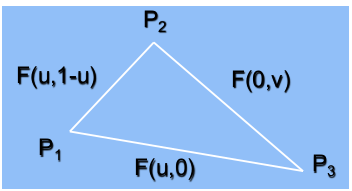
\includegraphics[width=.3\linewidth]{figures/ch02_dreieck.png}
\end{center}
\end{itemize}
Oder sie werden durch \textbf{Bilineare Viereckselemente / Pflaster} approximiert:
\begin{itemize}
\item[] Gegeben sind 4 Punkte im Raum $P_1 , P_2 , P_3, P_4$
\item[] Damit wird die Fläche definiert durch $F(u,v)=(1-u)(1-v) \cdot P_1 + (1-u)v \cdot P_2 + u(1-v) \cdot P_3 + uv \cdot P_4$ mit $0 \leq u \leq 1, 0 \leq v \leq 1$. 
\begin{center}
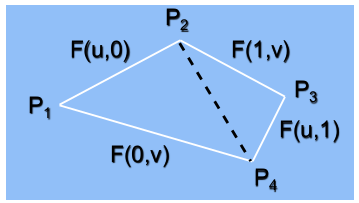
\includegraphics[width=.3\linewidth]{figures/ch02_pflaster.png}
\end{center}
\end{itemize}
\begin{table}[hbt]
\centering
\begin{tabular}{|p{6.5cm}|p{6.5cm}|}
\hline
Vorteile & Nachteile\\
\hline
\vspace{-5mm}
\begin{itemize}
\setlength\itemsep{0em}
\item[+] Flächenelemente können gekrümmt sein
$\rightarrow$ weniger Gitterpunkte bei gleich guter Approximation
\end{itemize}
 &
 \vspace{-5mm}
\begin{itemize}
\setlength\itemsep{0em}
\item[-] Rechnen mit gekrümmten Flächen ist aufwendig
\end{itemize}\\
\hline
\end{tabular}
\caption{Approximation durch Vierecke}
\label{tab:Viereck_approx}
\end{table}
Zudem können Flächen durch \textbf{Bezierflächen}, einer Erweiterung der Bezierkurven beschrieben werden:
\begin{itemize}
\item[] Gegeben ist ein Gitter von Führungspunkten $P_{ij}, 0 \leq i \leq N$ und $0 \leq j \leq M$.
\item[] Damit ist die Fläche beschrieben durch $F(u,v) = \sum_{i=0}^N \sum_{j=0}^M P_{ij} \cdot B_{i,N}(u) \cdot B_{j,M}(v)$\\
 mit $B_{i,N}(u) = (1-u)B_{i,N-1}(u)+uB_{i-1,N-1}(u)$\\
 und $B_{j,M}(v) = (1-v)B_{j,M-1}(v)+vB_{j-1,M-1}(v)$.
\item[] Die $B_{i,N}$ bzw. $B_{j,M}$ heißen auch Bernsteinpolynome.
\begin{center}
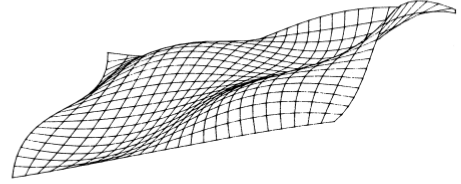
\includegraphics[width=.4\linewidth]{figures/ch02_bezier.png}
\end{center}
\end{itemize}
\begin{table}[hbt]
\centering
\begin{tabular}{|p{6.5cm}|p{6.5cm}|}
\hline
Vorteile & Nachteile\\
\hline
\vspace{-5mm}
\begin{itemize}
\setlength\itemsep{0em}
\item[+] effiziente Verfahren 
\item[+] entspricht dem Vorgehen während der Modellierung
\item[+] schnelle Kollisions- und Abstandsberechnung
\end{itemize}
 &
 \vspace{-5mm}
\begin{itemize}
\setlength\itemsep{0em}
\item[-] hoher Eingabeaufwand
\item[-] Darstellung aufwendig
\item[-] Problem bei Schnittoperationen
\item[-] Inkonsistenzen möglich
\end{itemize}\\
\hline
\end{tabular}
\caption{Zusammenfassung -- Flächenmodelle}
\label{tab:Flaechenmod}
\end{table}
\noindent
\paragraph*{Volumen} Vier verschiedene Arten von Volumenmodellen:\\ \\
\textbf{Parametrische Modelle}:\\
Grundkörper und topologische Operationen auf diesen (Schnitt, Vereinigung, ... ) werden abgespeichert. 
\begin{table}[hbt]
\centering
\begin{tabular}{|p{6.5cm}|p{6.5cm}|}
\hline
Vorteile & Nachteile\\
\hline
\vspace{-5mm}
\begin{itemize}
\setlength\itemsep{0em}
\item[+] eindeutige Objektbeschreibung 
\item[+] geringer Eingabeaufwand 
\item[+] Ergebnis von Operationen sind korrekte Objekte
\end{itemize}
 &
 \vspace{-5mm}
\begin{itemize}
\setlength\itemsep{0em}
\item[-] hoher Implementierungsaufwand
\item[-] Einbindung von Freiformflächen schwierig
\end{itemize}\\
\hline
\end{tabular}
\caption{Volumenmodelle -- parametrisch}
\label{tab:Volmod}
\end{table}\\ 
Die Objekte sind bereits vorhanden und können durch Angabe von Parametern angepaßt werden (Varianten).\\
Konsistenzprüfungen sind notwendig (\autoref{fig:kons})! \\
\begin{figure}[h!]
	\centering 
	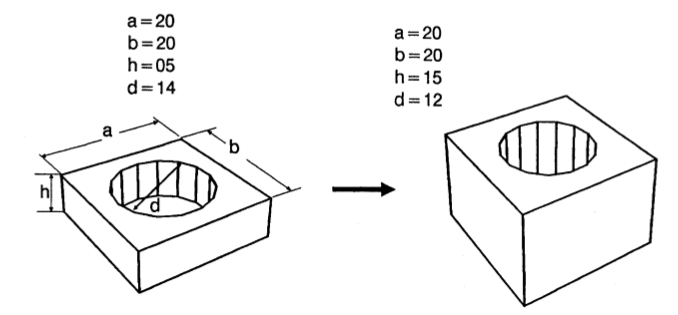
\includegraphics[width=0.3\linewidth]{figures/ch02_kons.png}
	\caption{Konsistenzprüfung: $d < min(a,b)$}
\label{fig:kons}
\end{figure}\\
\noindent
\textbf{Zellenzerlegung}:\\
 Objekte werden aus disjunkten Elementarzellen aufgebaut. Verwendung finden einfache geometrische Objekte z,B. Tetraeder, Quader, ...
Benutzt in der Strukturanalyse mit Finite-Elemente-Methoden (FEM).
\newpage
Diese Modelle können auf drei Arten umgesetzt werden:
\begin{enumerate}
\item Boundary Repräsentation
\item Constructive Solid Geometry (CSG)
\item Zellenbelegung
\end{enumerate}
\textbf{Boundary Repräsentation}: Hierarchische Darstellung eines Objektes durch begrenzende
Elemente, i.d.R. Kanten oder Flächen. \autoref{fig:brep} zeigt ein Beispiel.\\
\begin{figure}[h!]
	\centering 
	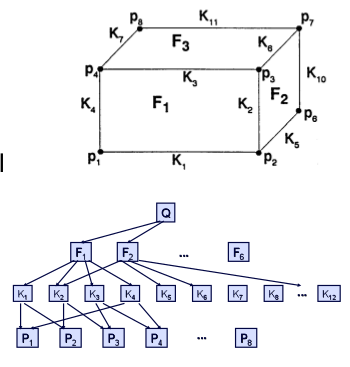
\includegraphics[width=0.3\linewidth]{figures/ch02_brep.png}
	\caption{Elemente eines Quaders im Flächenmodell: Quader $Q$, Flächen $F_i : i \in \{1,...,6\}$, Kanten $K_i : i \in \{1,...,12\}$, Ecken $P_i : i \in \{1,...,8\}$}
\label{fig:brep}
\end{figure}
Vorteile: aus der topologischen Struktur Information über z.B.:
\begin{itemize}
\item Welche Flächen gehören zum Objekt?
\item Welche Kanten gehören zur Fläche? $\rightarrow$ kantenbasierte Objekterkennung
\item Zu welchem Objekt gehört eine Fläche?
\item Zu welchem Objekt gehört eine Kante?
\item Welche Flächen stoßen aneinander?
\end{itemize}
\noindent
\textbf{Constructive Solid Geometry (CSG)}:
Es gibt eine Menge von einfachen Grundkörpern, die parametriert
werden können (\autoref{fig:csg}). 
\begin{figure}[h!]
	\centering
	\begin{subfigure}{.7\textwidth}
		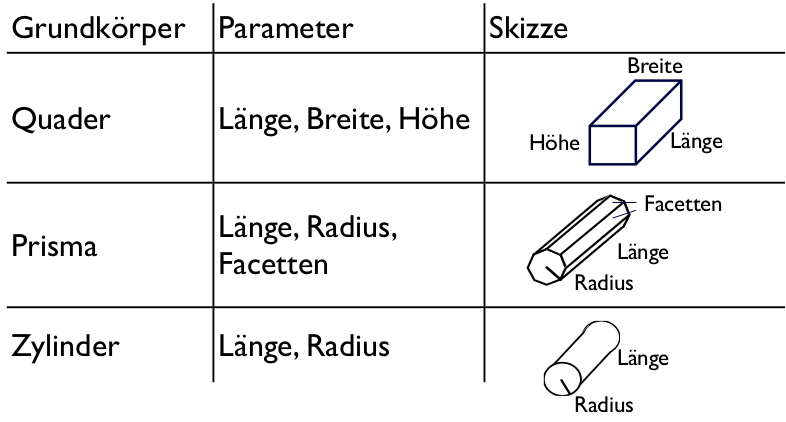
\includegraphics[width=\textwidth]{figures/ch02_csg.png}
	\end{subfigure}
	\begin{subfigure}{.7\textwidth}
		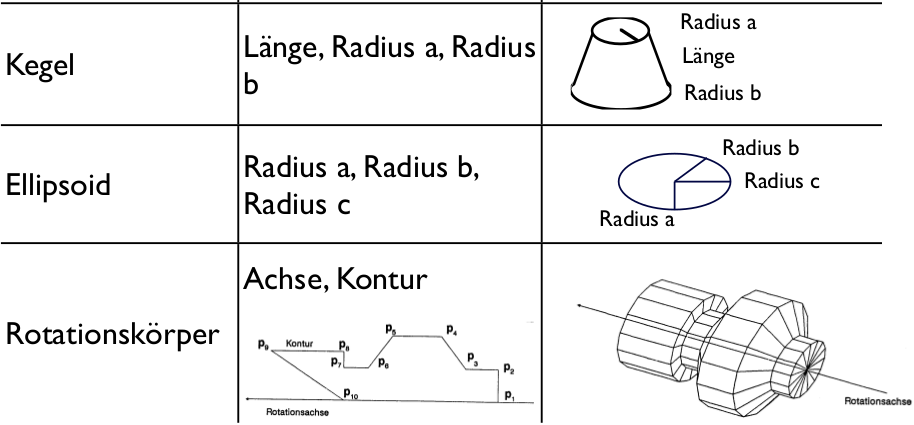
\includegraphics[width=\textwidth]{figures/ch02_csg1.png}
	\end{subfigure}
	\caption{Constructive Solid Geometry}
	\label{fig:csg}
\end{figure}
Auf ihnen sind verschiedene Operationen definiert, z.B.
\begin{table}[!hb]
\centering
\begin{tabular}{|p{6.5cm}|p{6.5cm}|}
\hline
Objekt $A$ 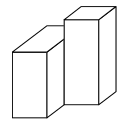
\includegraphics[width=.07\textwidth]{figures/ch02_a.png} & Objekt $B$ 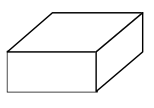
\includegraphics[width=.07\textwidth]{figures/ch02_b.png}\\
\hline
Vereinigung $A \cup B$ (Summe) & 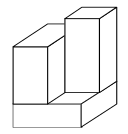
\includegraphics[width=.07\textwidth]{figures/ch02_ab.png}\\
\hline
Schnitt $A \cap B$ & 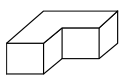
\includegraphics[width=.07\textwidth]{figures/ch02_ab1.png} \\
\hline
Differenz $A / B$ & 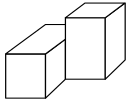
\includegraphics[width=.07\textwidth]{figures/ch02_ab2.png}\\
\hline
Sweep:
Ein Grundelement (u.U. eine Fläche) wird entlang einer Raumkurve
verschoben. Der durchdrungene Raum stellt das neue Objekt dar. & \\
\hline
\end{tabular}
\caption{CSG -- Operatoren}
\label{tab:csg_ops}
\end{table}\\ \\
\textbf{Zellenbelegung}:
Der Raum wird in mehrere Zellen unterteilt (i.d.R. 8 Zellen: \glqq Octree\grqq).
Wenn eine Zelle komplett vom Objekt belegt ist, als \glqq belegt\grqq{} markieren.
Wenn die Zelle nur teilweise belegt ist, dann wird auf diese Zelle das
Verfahren rekursiv angewendet. Ansonsten ist die Zelle leer.
Die Rekursion terminiert bei einer vorbestimmten minimalen Zellgröße.
Teilbelegte kleinste Zellen werden als belegt markiert. Siehe \autoref{zb}.
\begin{figure}[h!]
	\centering
	\begin{subfigure}{.45\textwidth}
		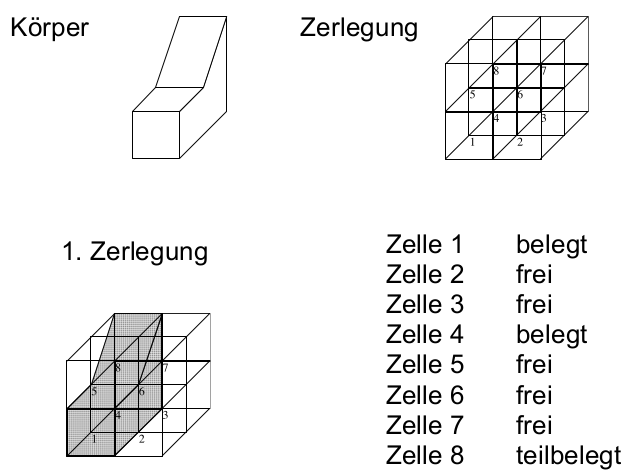
\includegraphics[width=\textwidth]{figures/ch02_zb.png}
	\end{subfigure}
	\begin{subfigure}{.45\textwidth}
		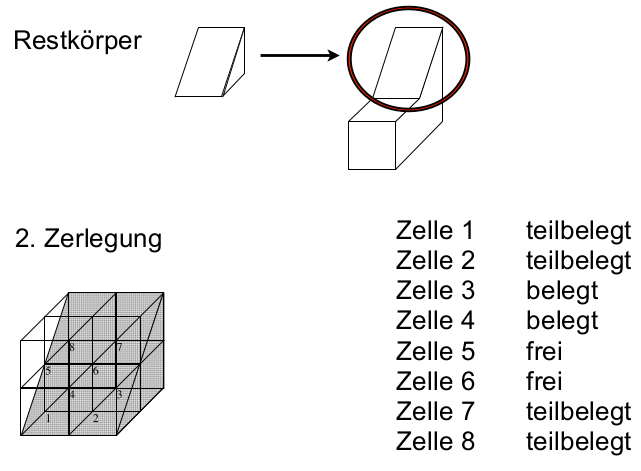
\includegraphics[width=\textwidth]{figures/ch02_zb1.png}
	\end{subfigure}
	\caption{Beispiel -- Zellenbelegung}
	\label{zb}
\end{figure}
\newpage
\subsection{Aufgabenmodellierung}
\begin{figure}[h!]\centering 
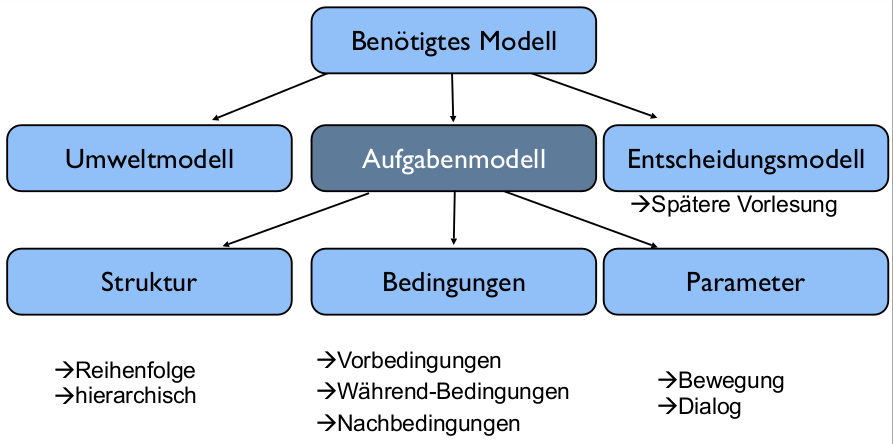
\includegraphics[width=0.6\linewidth]{figures/ch02_aufgabenmodell.png}
\caption{Aufgabenmodell}
\label{fig:ch02_am}
\end{figure}
%kognitive Lücke?
\begin{figure}[ht]\centering 
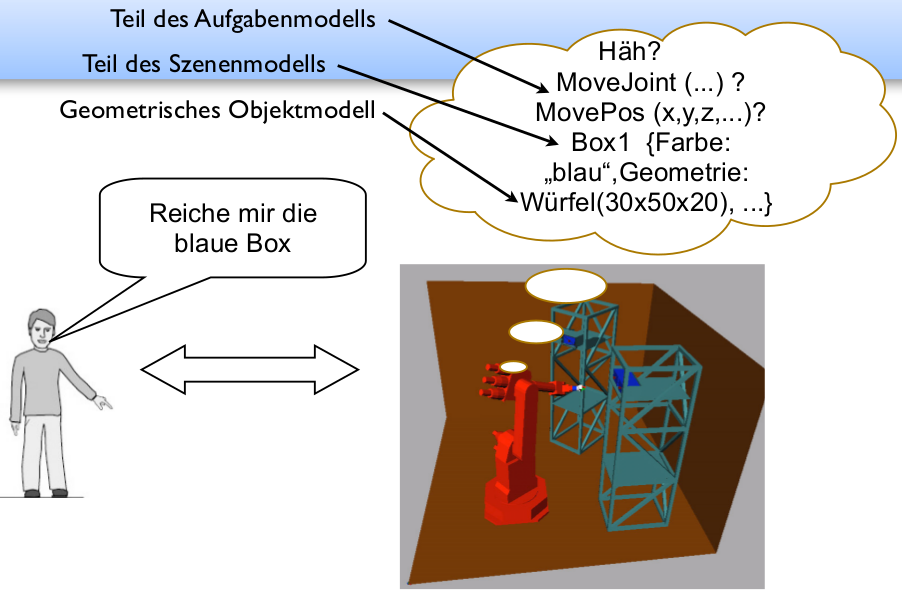
\includegraphics[width=0.6\linewidth]{figures/ch02_beispiel.png}
\caption{Beispiel}
\label{fig:ch02_bsp}
\end{figure}
\begin{figure}[h!]\centering 
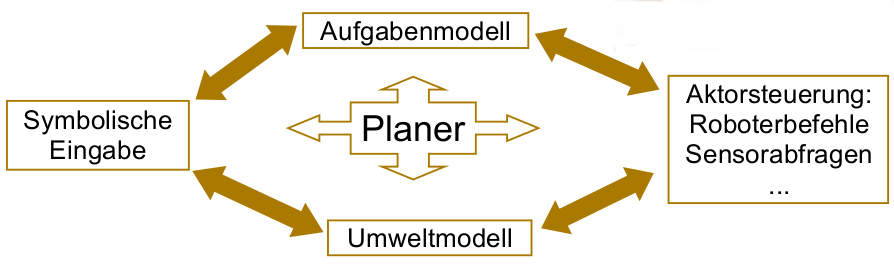
\includegraphics[width=0.6\linewidth]{figures/ch02_planer.png}
\caption{Einordnung des Aufgabenmodells}
\label{fig:ch02_ord}
\end{figure}
\textbf{Anforderungen an das Aufgabenmodell}:
\begin{itemize}
\item Erweiterbarkeit
\item Erklärbarkeit
\item Wiederverwendbarkeit
\item Integration des Wissens in ein Planungssystem
\end{itemize}
\newpage
\paragraph*{Symbolische Abstraktion}
Benutzer beschreibt die Aufgabe mit seinen Worten\\ (z.B. \glqq Bring mir Tee!\grqq) 
\begin{itemize}
\ita Abbildung: Erzeugung der Roboterbefehle über mehrere Stufen (vgl. \autoref{symbab})
\ita \glqq Fahre in die ‚Küche‘, greife ein Glas, fahre zurück und reiche mir den Becher.\grqq
\ita \glqq DriveTo(...), SearchObject(...), MoveArm(...), Grasp(Becher), MoveArm(...), DriveTo(...), MoveArm(...) ...!\grqq
\end{itemize}
\begin{figure}[h!]\centering 
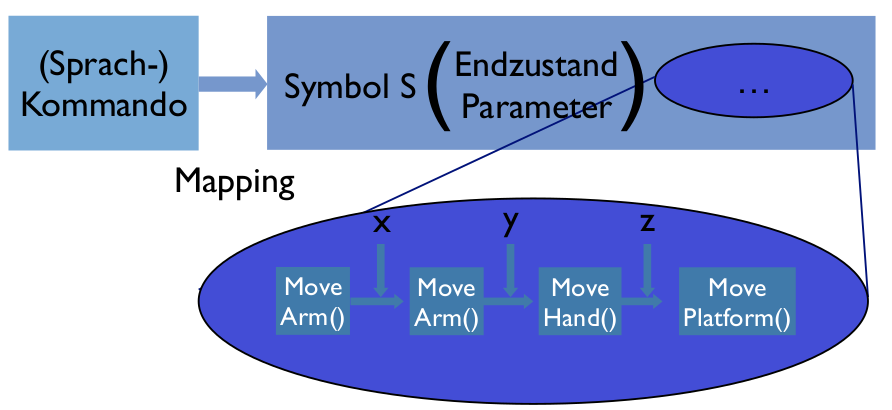
\includegraphics[width=0.6\linewidth]{figures/ch02_symbab.png}
\caption{Symbolische Abstraktion}
\label{symbab}
\end{figure}
\paragraph*{Modellierung der Reihenfolge von Operatoren/Symbolische Handlungsatome}
\begin{itemize}
\item In den gegebenen Beispielen wurden bereits implizit Handlungsatome angenommen
\item Die kleinsten auszuführenden Handlungseinheiten werden als
Elementaroperationen oder atomare Handlungen bezeichnet.
\item Komplexe Handlungen werden aus Elementaroperationen zusammengesetzt. Diese
können dazu üblicherweise parametriert werden.
\item Jeder Roboter besitzt eine endliche Menge an Elementaroperationen.
\end{itemize}
\paragraph*{Drei Ansätze für das Aufgabenmodell}
\begin{enumerate}
\item Sequentiell (\autoref{seq}): Festgelegte Folge von elementaren Aktionen 
\item Vorranggraph (\autoref{vorgra}): Darstellung der Abhängigkeiten
\item Hierarchisch (\autoref{hierar}): Abstraktion von Teilhandlungen
\end{enumerate}
\begin{figure}[h!]
	\centering
	\begin{subfigure}{.25\textwidth}
		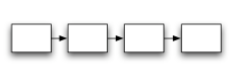
\includegraphics[width=\textwidth]{figures/ch02_ans.png}
		\caption{Sequentiell}
		\label{seq}
	\end{subfigure}
	\begin{subfigure}{.25\textwidth}
		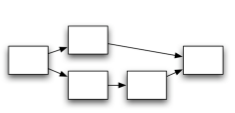
\includegraphics[width=\textwidth]{figures/ch02_ans1.png}
		\caption{Vorranggraph}
		\label{vorgra}
	\end{subfigure}
		\begin{subfigure}{.25\textwidth}
		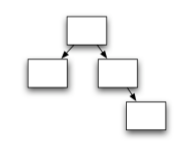
\includegraphics[width=\textwidth]{figures/ch02_ans2.png}
		\caption{Hierarchie}
		\label{hierar}
	\end{subfigure}
	\caption{Ansätze für das Aufgabenmodell}
	\label{ans}
\end{figure}
\newpage
\textbf{Sequentielle Handlungsbeschreibung}:
\begin{itemize}
\item Folge von (parametrierten) atomaren Handlungen
\item Eindeutig festgelegte Reihenfolge
\item Reihenfolge und Anordnung nicht unbedingt erklärbar (lesbar)
\item Bedingungen, Alternativen, etc. schlecht darstellbar
\item Sinnvoll für einfache Aufgaben oder sehr strukturierte Umgebungen (z.B. Leittechnik/Industrie)
\item Komplexe Handlungen: Rein sequentielle Beschreibungen nicht mächtig genug!
\item Ausführung sequentiell beschriebener Handlungen trivial
\item Linearer Handlungsfluss
\item Ausführung besteht aus: Anstoßen einer Elementarhandlung, evtl. Handlungsüberwachung und nach (erfolgreicher) Beendigung Übergang zur nächsten Elementarhandlung
\item Einfache Mechanismen zur Ausführung nötig!
\end{itemize}
\textbf{Vorranggraph}:
\begin{figure}[h!]
	\centering
	\begin{subfigure}{.45\textwidth}
		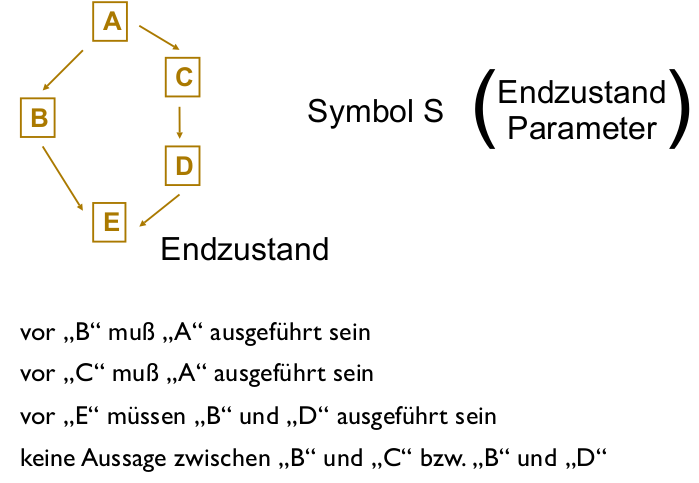
\includegraphics[width=\textwidth]{figures/ch02_vg-mod.png}
		\caption{Modellierung der Reihenfolge: Vorranggraph}
	\end{subfigure}
	\begin{subfigure}{.45\textwidth}
		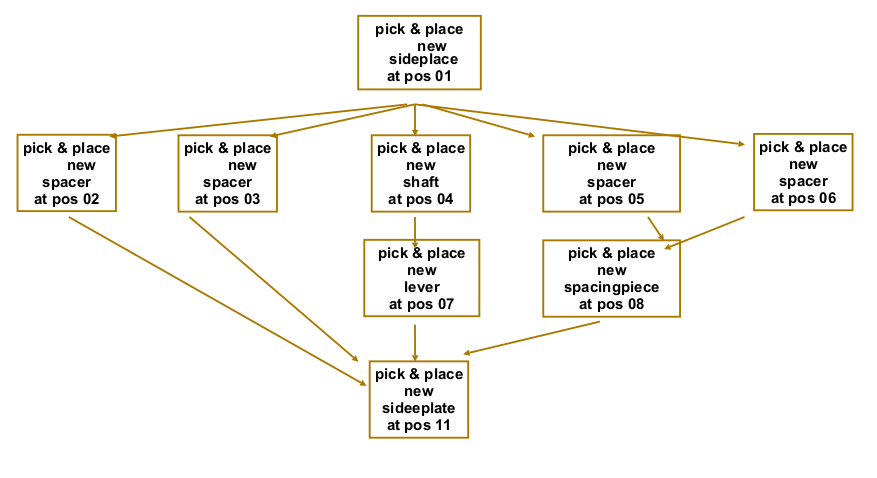
\includegraphics[width=\textwidth]{figures/ch02_vg-bsp.png}
		\caption{Beispiel: Vorranggraph des Cranfield-Benchmarks (simple Montage-Aufgabe)}
		\label{vg}
	\end{subfigure}
	\caption{Vorranggraph}
	\label{vg1}
\end{figure}
\begin{itemize}
\item Darstellung der Handlung in mehreren unabhängigen Teilzweigen
\item Üblicherweise: Serialisierung notwendig!
\begin{itemize}
\item Berechnung optimaler Operatorreihenfolgen
\item Freiheitsgrad zum Ausführungszeitpunkt
\item Serialisierung aufwendig ($\rightarrow$ Planungsverfahren, siehe spätere Vorlesungen)
\end{itemize}
\item Ausführung beinhaltet also:
\begin{itemize}
\item Serialisierung der Handlung nach gegebenen Kriterien
\item Ausführung der sequentiell beschriebenen Handlung
\end{itemize}
\item Mächtigere Handlungsbeschreibung benötigt auch mächtigere Verfahren bei der Ausführung!
\end{itemize}
\textbf{Hierarchisches Aufgabenmodell} (Abbildungen \ref{hier} und \ref{hiermod}):\\
Sowohl Aufgabenspezifikation als auch Aufgabenzerlegung/-teilung sind hierarchisch strukturiert. Die Abstraktion erfolgt nach Raum, Zeit, Objekten und Alternativen.
\begin{figure}[h!]\centering 
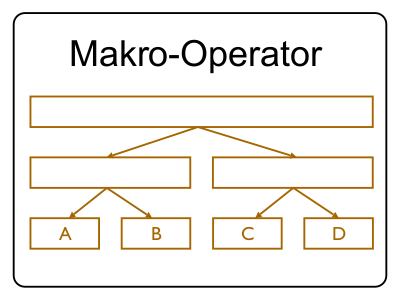
\includegraphics[width=0.3\linewidth]{figures/ch02_hier.png}
\caption{}
\label{hier}
\end{figure}\\
\begin{figure}[h!]
	\centering
	\begin{subfigure}{.45\textwidth}
		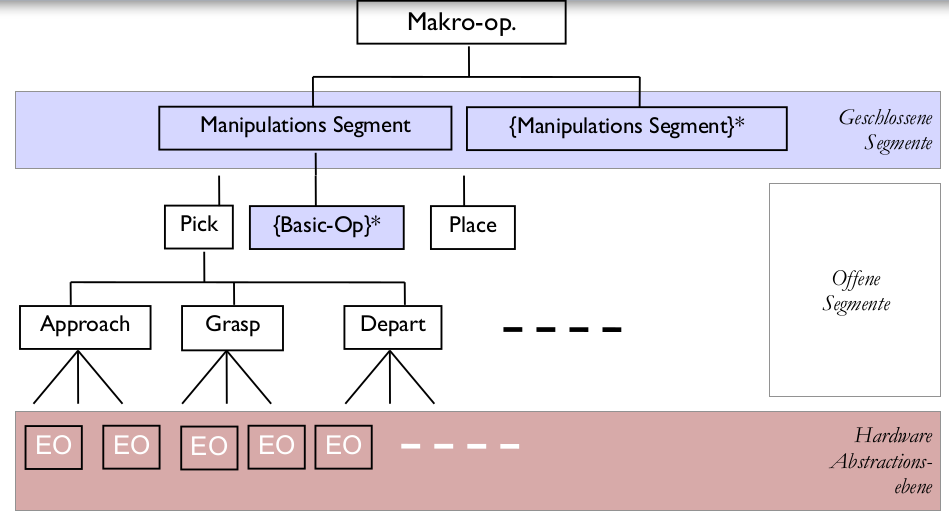
\includegraphics[width=\textwidth]{figures/ch02_hier1.png}
		\caption{Semantische hierarchische Repräsentation}
	\end{subfigure}
	\begin{subfigure}{.45\textwidth}
		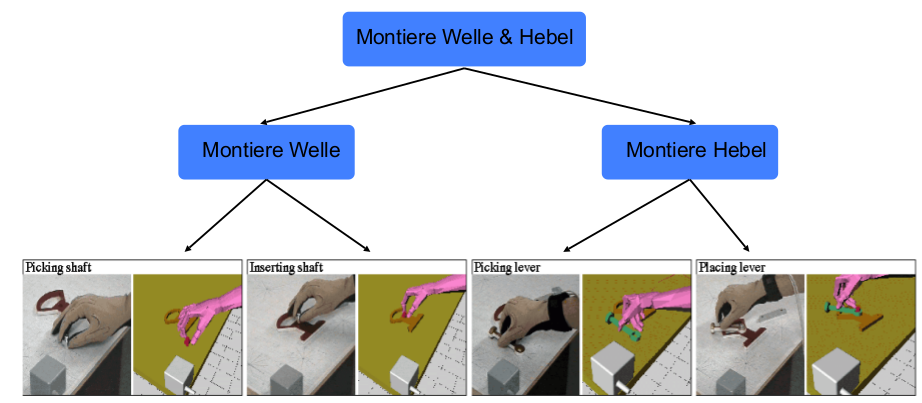
\includegraphics[width=\textwidth]{figures/ch02_hier2.png}
		\caption{Programmbeispiel: Montage von Welle und Hebel des Cranfield Benchmarks}
	\end{subfigure}
	\caption{Hierarchisches Aufgabenmodell}
	\label{hiermod}
\end{figure}
\paragraph*{Abstraktionsebenen im Aufgabenmodell}
Häufige Unterscheidung der in \autoref{abst} dargestellten semantischen Abstraktionsstufen. Diese benutzen symbolische Parameter.
\begin{itemize}
\ita Komplexität der Aufgabe beherrschbar
\ita Formalismen anwendbar
\end{itemize}
\begin{figure}[h!]\centering 
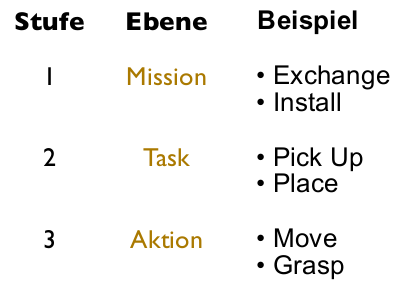
\includegraphics[width=0.3\linewidth]{figures/ch02_abst.png}
\caption{}
\label{abst}
\end{figure}
\textbf{Wahl der Abstraktionsebene}: Wie wird die Abstraktionsebene der Aktion gewählt, damit Aktionen von Roboter A auf Roboter B übertragen werden können?
\begin{itemize}
\item Aktion: Kleinste symbolische Einheit
\item Darunter: Regelungsebene
\item Abhängig von:
\begin{itemize}
\item Komplexität der Aufgabe
\item Grad der Kopplung einzelner Teilhandlungen
\item Hardware: Getrennt geregelte Komponenten werden üblicherweise auch mit getrennten Aktionen modelliert
\item Planungssystem/Beobachtungssystem
\end{itemize}
\item Grundsätzlich: Die Frage ist in der Forschung noch nicht eindeutig geklärt, immer noch ein Streitpunkt!
\end{itemize}
\textbf{Modellierung von Aktionen / Tasks}:\\
Ein \textcolor{red}{Operator} ist definiert durch $OP = (N, O, A, Par, K)$ mit
\begin{itemize}
\item $N$ = Name des Operators (eindeutig)
\item $O$ = Liste der beteiligten Objekte
\item $A$ = Auswahlbedingung
\item $Par$ = Liste der Parameter, z.B. Positionen, Kräfte, Beschleunigungen ...
\item $K$ = Körper des Operators:
\begin{itemize}
\item \textcolor{red}{\textbf{Aktion}/Elementaroperator}:\\ ausführbares Programm\\ $\Rightarrow$ Realisierung einfacher Fähigkeiten
\item \textcolor{red}{\textbf{Task}/Makro-Operator}:\\ besteht aus weiteren Operationen $K = K_1K_2...K_n$ $\Rightarrow$\\ Realisierung einfacher Fähigkeiten
\end{itemize}
\end{itemize}
\textbf{Hierarchische Repräsentation -- Ausführung}:
\begin{itemize}
\item Im Aufgabenmodell ist die Serialisierung implizit gegeben
\begin{itemize}
\item Minimaler Aufwand zur Ausführung
\item Aber: Bei Parallelitäten von Teilhandlungen: Konflikte möglich!
\end{itemize}
\item Ausführung beinhaltet also:
\begin{itemize}
\item Überprüfung auf Konflikte
\item Gegebenenfalls Serialisierung/Lösen der Konflikte
\item Ausführung der resultierenden Operatorsequenz
\end{itemize}
\item Vorteil: Zusammengesetzte (Teil-)Programme können wiederverwendet werden
\item Repräsentation gut \glqq lesbar\grqq{} (verständlich, erklärbar)
\end{itemize}
\textbf{Anwendung hierarchischer Handlungsbeschreibung in der Realität  \\-- Flexible Programme}:\\
Symbolische Abstraktionsebene zur Roboterprogrammierung
\begin{itemize}
\item Hierarchische Handlungsbeschreibung
\item Erklärbar, verständlich, intuitiv
\item Wiederverwendbarkeit
\item Parametrierbar
\item Unterstützt: Bedingungen, Verzweigungen, Ressourcenverwaltung, Parallelität
\item Aufbau flexibler Programme:
\begin{itemize}
\item Repräsentation des Handlungswissens als Baumstruktur
\item Parametrierbare Aktionsbeschreibung
\item Blätter entsprechen Roboteraktionen
\item Abarbeitung entsprechend einer Tiefensuche
\item Instantiierung der Kinder zur Laufzeit (Expansion des Baums)
\item Auswahl des geeignetsten Kandidaten beim expandieren
\item Parallele Ausführung mehrerer Kinder möglich
\end{itemize}
\end{itemize}
\paragraph*{Validierung der Modelle: Simulation oder Graphische Animation}
\begin{enumerate}
\item \textbf{Simulation der Komponenten}: Validierung anhand gegebener Einschränkungen (Kollisionen, Erreichbarkeit, Optimalitätskriterien: Weg, Zeit, Energie, ...)
\begin{itemize}
\ita Für die Simulation von Effekten durch Manipulators wird die Physiksimulation verwendet: Masse, Reibung, Kräfte, Gelenke
\end{itemize}
\item \textbf{Graphische Animation}: Der Anwender überprüft visuell die erstellten Modelle
\begin{itemize}
\ita Wenn die Robotersimulationen ergeben, dass die Zielstellung angefahren werden kann, wird die Bewegung in einer Animation graphisch dargestellt.
\end{itemize}
\end{enumerate}

\paragraph*{Aufgabenmodell -- Zusammenfassung und Diskussion}:\newline
\textbf{Zusammenfassung}:
\begin{itemize}
\item Aufgabenmodell basiert auf elementaren Operationen
\item Oft dreischichtiger Ansatz: Aktion, Task, Mission
\item Verknüpfung der elementaren Operationen zu komplexen Aufgaben:
\begin{itemize}
\item Sequentiell
\item Vorranggraph
\item  Hierarchisch
\item (Kontrollstrukturen)
\end{itemize}
\item Problem: Validierung der Programme
\begin{itemize}
\item Simulation
\item Animation und Validierung durch den Menschen
\end{itemize}
\end{itemize}

\textbf{Diskussion}:
\begin{itemize}
\item Mobile Plattform ohne Sensorik (z.B. Roomba)
\begin{itemize}
\item Aufgabenmodell?
\item Umweltmodell?
\end{itemize}
\item Mobile Plattform mit Differentialantrieb und Sensorik zur Lokalisation (z.B. Transportaufgaben)
\begin{itemize}
\item Aufgabenmodell?
\item Umweltmodell?
\end{itemize}
\item Serviceroboter mit mobiler Plattform, Manipulator, Mehrfingergreifer, komplexe Sensorik\begin{itemize}
\item Aufgabenmodell?
\item Umweltmodell?
\end{itemize}
\item Wo kommt jeweils das Aufgabenwissen dieser Systeme her?
\end{itemize}

\section{Interaktive Programmierung: Programmierung durch Vormachen von Manipulationsaufgaben} %(3.-5. VL)
\subsection{Grundlagen}
Neue Anforderungen an Robotersysteme:
\begin{itemize}
\item In der Produktion: Klein- \& Kleinstserienfertigung, Unikatfertigung (z.B. Prototyp)\\
$\rightarrow$ Produkte mit: vielen Ausstattungsvarianten und hoher Rekonfigurierbarkeit\\
$\rightarrow$ Flexible Fertigung
\item Im Servicebereich: \\
$\rightarrow$ Handel:  Kommissionierung und Palettierung von Waren, Bestücken von Regalen\\
$\rightarrow$ Pflege: Unterstützung von Rehabilitationsmaßnahmen durch Roboter, Rollstuhl mit Manipulationshilfe\\
$\rightarrow$ Handwerk: Handhabungen in Schreinereien und Schlossereien
\item In der humanoiden Servicerobotik: Manipulation beliebiger Objekte, selbstständiges Lösen komplexer Aufgaben, Einsatz im menschlichen Umfeld\\
$\rightarrow$ komplexe Umgebung und sehr viele Freiheitsgrade\\
$\rightarrow$ Wie Handlungswissen erzeugen?
\end{itemize}

\subsubsection*{Grundidee der interaktiven Programmierung} %5.1.1.
\begin{itemize}
\item[1.]Mensch ist Domänenexperte (Manipulation)
\item[2.]Explizite Demonstrationen der Manipulationsaufgabe
\item[3.]Sensorielle Erfassung der Demonstrationen
\item[4.]Erzeugung der internen Repräsentation des Roboterprogramms
\item[5.]Abbildung auf das Robotersystem
\item[6.]Ausführung
\end{itemize}

\subsubsection*{Anforderungen an interaktive Programmierung}
\begin{itemize}
\item[1.]Intuitive Interaktionsformen: einfache Bedienung des Systems
\item[2.]Transparenz der Prozesse im Programmiersystem: Umsetzung von Handlungen des Benutzers soll nachvollziehbar sein
\item[3.]Abgleich von Systemhypothesen mit der Benutzerintention: z.B. zur Korrektur falscher Systemhypothesen
\item[4.]Flexibilisierung und Optimierung von Programmen: erlernte Programme sollen in vielen Situationen anwendbar sein
\item[5.]Wiederverwendung von Teillösungen: Funktionsbausteine sollen in anderen Pogrammen wiederverwendbar sein
\end{itemize}

\subsubsection*{Randbedingungen}
Notwendig zur Erzeugung von leistungsfähigen, automatischen aber auch sicheren und komfortablen Roboterprogrammen
\begin{itemize}
\item[1.]Weitgehend automatisierte Programmgenerierung
\item[2.]Beschränkung der Benutzerinteraktion auf das Nötigste
\item[3.]Maximierung des Informationsgewinns und der Eindeutigkeit der Ergebnisse der Benutzerinteraktion für das System
\item[4.]Möglichst benutzerfreundliche Mensch-Maschine Interaktion: verständlich, transparent und flexibel, möglichst ähnlich zur zwischenmenschlichen Kommunikation
\end{itemize}

\subsection{PdV - Generelles Framework}
\begin{figure}[ht]\centering 
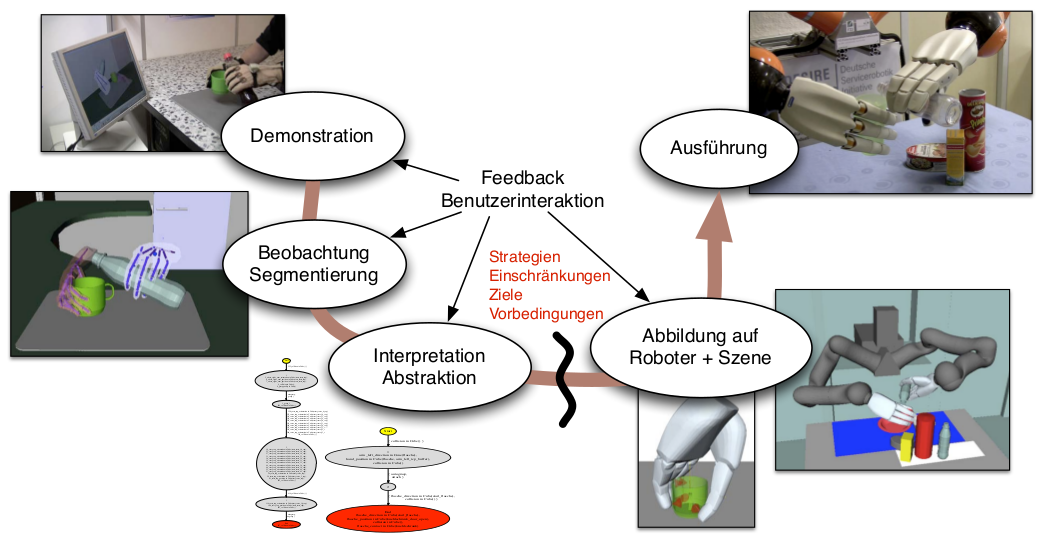
\includegraphics[width=0.6\linewidth]{figures/ch03_zyklus.png}
\caption{PdV-Zyklus}
\label{fig:ch03_zykl}
\end{figure}
Abbildung  \ref{fig:ch03_zykl} zeigt die Phasen von PdV.
\subsubsection*{Beobachtung}
Beobachtung der Benutzerinteraktion mittels externer und interner Sensorik (z.B. Kamerasysteme, Datenhandschuhe, Positionstracker).
\begin{itemize}
\ita mit den gewonnenen Sensordaten lassen sich dann Objekte klassifizieren, Trajektorien aufzeichnen und weitere Vorverarbeitungsschritte wie
Grifferkennung durchführen
\end{itemize}

\subsubsection*{Segmentierung}
Segmentierung in relevante Operationen oder Umweltzustände. 
\begin{itemize}
\item man benötigt hierfür die Trajektorien aus der Demonstration, eine Datenbasis mit den Sensordaten, einen Satz Aktionstypen (Griffe, Lageänderungen von Objekten), einen Satz
von Elementaroperationen und das Umweltmodell
\item durch eine geeignete Heuristik lässt sich damit die Segmentierung durchführen
\item eine zusätzlich Interaktion mit dem Benutzer (über verschiedene Kommunikationskanäle wie grafische Benutzerschnittstellen oder Sprache) hilfreich; 
Rückfragen helfen bei der Identifikation der in der Lösung involvierten Objekte und sparen damit unnötige Berechnungen aller Relationen zwischen allen Objekten
ein
\item Rauschfilterung
\end{itemize}
\subsubsection*{Interpretation/Abstraktion}
Abstraktion von der Demonstration um die Lösung der Aufgabe so allgemein wie möglich darzustellen.
\begin{itemize}
\ita Instanzen müssen falls möglich in Variablen umgewandelt werden; dabei muss sichergestellt werden, dass in der Ausführungsphase nur solche Variablen instantiiert
werden, die räumliche Vorbedingungen erfüllen. Es wird also für jeden \Gu generalisierten\Go Operator ein Satz von Vorbedingungen in Form von wichtigen Relationen
gespeichert. Generiert werden diese Vorbedingungen mit Hilfe von Hintergrundwissen und wiederum durch Rückfragen an den Benutzer. Man benötigt also eine deduktive
Komponente, die die generalisierten Operatoren in Makro-Operatoren gruppiert. Da Makro-Operatoren weitere Makro-Operatoren als Kinder beinhalten können, lässt
sich die gesamte Benutzervorführung auf verschiedenen Abstraktionsebenen darstellen. Durch die Generalisierung lässt sich die Lösung später auf ähnliche Problemklassen anwendbare Lösungsbeschreibungen abbilden. In dieser Phase lassen sich auch vom Demonstrator durchgeführte spontane und nicht zielorientierte Bewegungen ausfiltern.
\end{itemize}
\subsubsection*{Transfer/Abbildung auf Roboter \& Szene}
Transfer der internen Wissensrepräsentation auf das Zielsystem. Aus den zuvor gewonnenen semantischen Informationen lässt sich jetzt ein ausführbares Roboterprogramm generieren. Dafür müssen die Operationen auf die Operationen des Zielsystems abgebildet werden. Die Ausgabe dieser Phase ist eine Sequenz von Elementarbewegungen, die nur für das Zielsystem und das jeweilige Umweltmodell gültig sind. Diese kann direkt in das Simulationsmodul weitergeleitet werden.
\subsubsection*{Simulation}
Simulation des physikalischen Vorgangs zur Validierung der getroffenen Entscheidungen. In der Simulation wird die gelernte Aufgabe von einem virtuellen Modell des Roboters in einer virtuellen Umwelt an virtuellen Objekten ausgeführt. Anhand einer visuellen Ausgabe lässt sich vom Benutzer die korrekte Ausführung der Aufgabe überprüfen. 
\subsubsection*{Ausführung}
Ausführung auf dem Zielsystem. Die zuvor validierte Sequenz elementarer Roboterbewegungen wird an den Roboter-Controller weitergereicht. Wenn bei der Modellierung in der Simulationsphase keine Fehler gemacht wurden, ist es sehr wahrscheinlich, dass die Ausführung nicht fehlschlagen wird-

\subsection{Klassifikation von PdV-Verfahren}
\begin{figure}[ht]\centering 
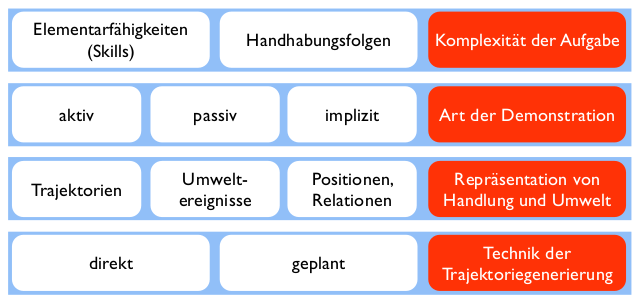
\includegraphics[width=0.6\linewidth]{figures/ch03_kriterien.png}
\caption{Klassifikationskriterien}
\label{fig:ch03_krit}
\end{figure}
Abbildung  \ref{fig:ch03_krit} zeigt die Klassifikationskriterien auf einen Blick.
\subsubsection*{Komplexität der Aufgabe}
Siehe Tabelle \ref{tab:aufgkomp}
\begin{table}[hbt]
\centering
\begin{tabular}{|p{8cm}|p{8cm}|}
\hline
Elementarfähigkeiten & Komplexe Aufgaben\\
\hline
Reflexe, Basisskills, einfache Bewegungen 
\vspace{-4mm}
\begin{itemize}
\setlength\itemsep{0em}
\item Lernen direkter Sensor-/Aktorzusammenhänge
\item Beispiele: Verwendung neuronaler Netze auf adaptive Regelkreise, Zustandsautomaten \footnote{Asada91, Koeppe95, Kaiser96, Ishikawa99, Bentivegna00, Calinon08, Pastor09}
\item[$\rightarrow$] Probleme: Explizite Beispiele, stark konfigurationsabhängig,
viele Trainingsbeispiele notwendig
\end{itemize}
 &
Task, Montageaufgaben
 \vspace{-4mm}
\begin{itemize}
\setlength\itemsep{0em}
\item Interpretation von Handlungsfolgen\footnote{Segre89, Inaba90, Kang94, Sagerer98, Aleotti06, Pardowitz07
Veeraraghavan08}
\ita Probleme: Breites Hintergrund-, Planungs- und Modellwissen,
Klärungsdialoge mit dem Benutzern
\end{itemize}\\
\hline
\end{tabular}
\caption{Kriterium 1 - Komplexität der Aufgabe}
\label{tab:aufgkomp}
\end{table}
\subsubsection*{Art der Demonstration}
Siehe Tabelle \ref{tab:demo}
\begin{table}[hbt]
\centering
\begin{tabular}{|p{5cm}|p{5cm}|p{5cm}|}
\hline
aktiv & passiv & implizit\\
\hline
Aktive Beispiele
\vspace{-4mm}
\begin{itemize}
\setlength\itemsep{0em}
\item Benutzer führt explizit vor
\item Beobachtung durch Sensorsystem (Datenhandschuh, Kameras)\footnote{Friedrich98, Ikeuchi99, Inoue/Kuniyoshi94, Zöllner06}
\ita Probleme: Aufwendige Sensorsysteme, Identifikation relevanter Aktionen und Ziele bzw. Zustände schwierig
\end{itemize}
 &
Passive Beispiele
 \vspace{-4mm}
\begin{itemize}
\setlength\itemsep{0em}
\item Roboter wird duch externen \Gu Master\Go
gesteuert, Signalaufzeichnung, Korrelation
zwischen Sensor- und Aktordaten\footnote{Kaiser96, Koeppe98, Billard07}
\ita Probleme: Gelerntes Wissen ist auf
konkretes Zielsystem festgelegt
\end{itemize} 
&
Implizite Beispiele
 \vspace{-4mm}
\begin{itemize}
\setlength\itemsep{0em}
\item Zielspezifikation durch Vorgabe graphischer Ikone\footnote{Takahashi/Ogata97,Sagerer98, Riepp97}
\ita Probleme: Dialog umfangreich, Anpassung an Zielsystem
\end{itemize}\\
\hline
\end{tabular}
\caption{Kriterium 2 - Art der Demonstration}
\label{tab:demo}
\end{table}

\subsubsection*{Repräsentation von Handlung und Umwelt}
Siehe Tabelle \ref{tab:rep}
\begin{table}[hbt]
\centering
\begin{tabular}{|p{5cm}|p{5cm}|p{5cm}|}
\hline
Trajektorien & Umweltereignisse & Positionen, Relationen\\
\hline
\vspace{-4mm}
\begin{itemize}
\setlength\itemsep{0em}
\ita Problem: keine wesentliche Generalisierung (1:1 Abbildung)
\end{itemize}
 &
Wirkungen und Reaktionen auf die Umgebung
 \vspace{-4mm}
\begin{itemize}
\setlength\itemsep{0em}
\ita Probleme: Identifikation von Kausalitäten und
Zustandsfolgen durch kognitive Operatoren
\end{itemize} 
&
Objektlagen, Relationen und Operatoren
 \vspace{-4mm}
\begin{itemize}
\setlength\itemsep{0em}
\ita Probleme: Beschränkung auf vorgegebenen
Operatorumfang
\end{itemize}\\
\hline
\end{tabular}
\caption{Kriterium 3 - Repräsentation von Handlung und Umwelt}
\label{tab:rep}
\end{table}
\subsubsection*{Technik der Trajektoriengenerierung}
Siehe Tabelle \ref{tab:trajtech}
\begin{table}[hbt]
\centering
\begin{tabular}{|p{8cm}|p{8cm}|}
\hline
direkt & geplant\\
\hline
Planung von Roboterbewegungen / Aktionen
\vspace{-4mm}
\begin{itemize}
\setlength\itemsep{0em}
\item Planung erforderlich zur Berücksichtigung der Unterschiede in
Demonstrations- und Ausführungsumgebung
\item Vollständige Nutzung der Leistungsfähigkeit des Robotersystems
\ita Probleme: Umwelt- und Planungswissen erforderlich,
intelligentes Planungssystem
\end{itemize}
 &
Direkte Abbildung
 \vspace{-4mm}
\begin{itemize}
\setlength\itemsep{0em}
\item Explizites oder gelerntes Transformationsmodell\footnote{Kang97, Kaneko97}
\ita Probleme: Zielsystem und Zielumgebung müssen korrespondieren
\end{itemize}\\
\hline
\end{tabular}
\caption{Kriterium 4 - Technik der Trajektoriegenerierung}
\label{tab:trajtech}
\end{table}

\subsection{Prozesskomponenten der interaktiven Programmierung}
\begin{figure}[ht]\centering 
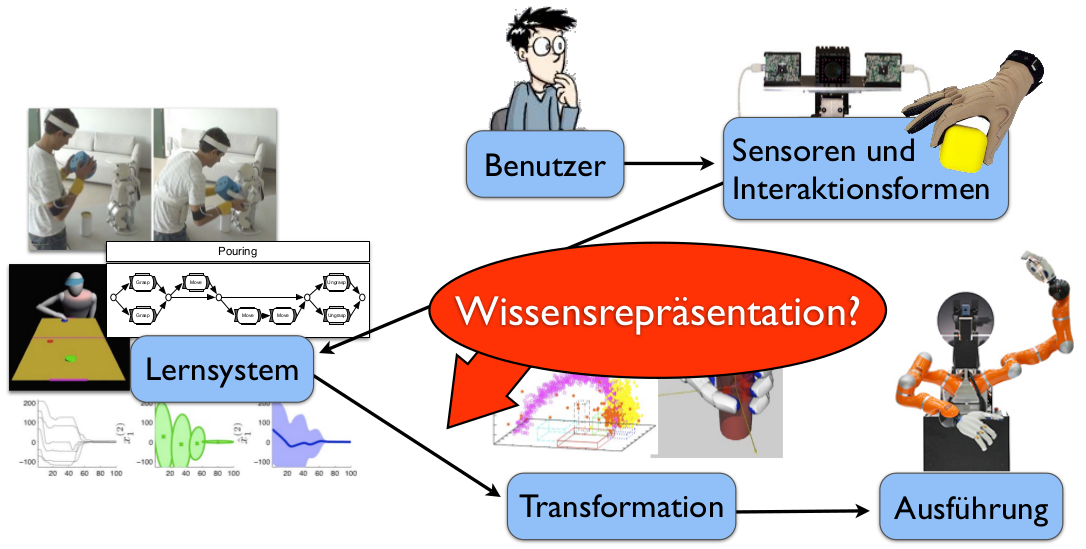
\includegraphics[width=0.6\linewidth]{figures/ch03_komponenten.png}
\caption{Interaktive Programmierung: Komponenten}
\label{fig:ch03_kom}
\end{figure}
Abbildung \ref{fig:ch03_kom} skizziert die an PdV beteiligten Komponenten:
\subsubsection*{Benutzer und Mensch-Maschine-Interaktionsformen}
Der Mensch, welcher die interaktive Programmierung vornimmt, kann multimodal mit dem Programmiersystem interagieren:
\begin{itemize}
\item \textbf{Physische Demonstration:}
Hierbei vollzieht der Benutzer die Manipulationsaufgabe mit realen Objekten und wird dabei
vom Programmiersystem durch Sensoren erfasst und seine Handlungen aufgezeichnet. 
Dies ist die natürlichste Art der Demonstration: Objekte können direkt mit den Händen 
oder mittels spezieller Vorführgeräte (z.B. Laserstift, 6D-Kugel) manipuliert werden. 
In jedem Fall ein großes Maß an Konzentration auf Seiten des Benutzers gefordert\\
Nachteile: 
\begin{itemize}
\item[-]Er muss sich weiterhin über die Beschränkung und Konfiguration der ihn beobachtenden Sensoren bewusst sein
(z.B. Verdeckung bei Beobachtung durch eine Kamera). Wegen der Abtastfrequenz der Sensoren
ist auch die Geschwindigkeit, mit der die Demonstration vorgeführt wird, zu beachten.
Oft ist es auch sinnvoll, die Manipulationsaufgabe in Teillösungen zu untergliedern, um
gegebenenfalls Fehler leichter zu beheben.
\item[-] Aufgrund der beschränkten sensorischen,
motorischen und intellektuellen Fähigkeiten des Menschen kann keine absolute 
Positioniergenauigkeit erwartet werden und auch die Wiederholgenauigkeit ist begrenzt.
\item[-] Auch produzieren menschliche Benutzer schon bei einfachen Manipulationsaufgaben häufig ineffiziente
oder überflüssige Handlungen. Ebenfalls tragen der Umfang und die Komplexität der Demonstration
der zu programmierenden Aufgabe dazu bei.
\end{itemize}
\item \textbf{Graphische Demonstration:} 
Der Benutzer kann hierbei die Manipulationsaufgabe lösen,
indem er 3D Objekte in einer simulierten Umgebung bewegt. Einige Probleme der physischen
Demonstration mit Sensoren (eingeschränkte Beobachtbarkeit, limitierte Genauigkeit, zeit-
licher Aufwand) sind bei dieser Art der interaktiven Programmierung nicht vorhanden. Es
wird versucht, die Vorteile der intuitiven physischen Demonstration zu übernehmen und
die angesprochenen Nachteile zu umgehen. Leider entstehen bei dieser Art von Demonstration
andere Probleme. Auf einem Monitor ist die Wiedergabe einer 3D Szene mit ihren zu manipulierenden
Objekten nur schwer zu erfassen. Sollen nur Translationen und Rotationen in einer Ebene ausgeführt
werden (z.B Bestückung einer Platine) reicht ein Monitor aus. Besser eigenen sich für die Darstellung
von 3D Umgebungen Datenhelme und Shutter Brillen sowie 3D Höhlen. Mit den
bisher beschriebenen Hilfsmitteln zur interaktiven Programmierung ist keine Möglichkeit
der Kraftrückkopplung gegeben. Haptischen Ein- und
Ausgabegeräte (Datenhandschuh mit Exoskelett und Phantom Manipulator) ermöglichen die Reaktionskräfte
an den Benutzer weiterzugeben. Er kann besser auf die simulierte Welt
einwirken, da er ein Feedback bekommt. Wegen der Echtzeitmodellaktualisierung ist aber
ein hoher Rechenaufwand nötig.\\
Diese ist für den menschlichen Benutzer mit den gleichen
Problemen verbunden wie die physische. Hinzukommen Probleme der Navigation und Koordination
in der simulierten Umgebung. Aufgrund der fehlenden Realität der virtuellen
Welt kann es sogar zu Simulationsübelkeit kommen. Dies geschieht durch den Widerspruch
der Signale, welche vom Gleichgewichts-, Orientierungs-, Seh- und Gehörsinn aufgenom-
men werden.
\item \textbf{Symbolische/Ikonische Demonstration:}
Es wird eine Aktionssequenz erzeugt, durch graphisches Aneinanderreihen vorhandener Teillösungen. 
Für diese Art der Demonstration reicht eine menügesteuerte, konventionelle graphische Schnittstelle.
Es müssen nur entsprechende Operatoren vorhanden sein, welche alle Informationen zur Manipulation
einzelner Objekte beinhalten. Die Ressourcenanforderungen an das System sind dementsprechend gering.
Bei ihr setzt der menschliche Benutzer aus
vorhandenen Teillösungen eine Lösung für die Manipulationsaufgabe zusammen. Das Problem
ist hierbei die Bestimmung der zu manipulierenden Objekte und die Parametrisierung
der Bewegungsfolge.
Die Kommentierung von Systemhypothesen, die Vermittlung der Sensorik von Aktionen
und der eigenen Intention ist für den Benutzer bei entsprechenden Benutzerschnittstellen
(symbolische, graphische Darstellung) leichter.
\item \textbf{Kommentierung:} Sie ist eine ergänzende Interaktionsform zur physischen oder 
graphischen Programmierung. Der Benutzer nimmt hierbei keine aktive Rolle ein, sondern reagiert
auf Systemhypothesen. Nach einer Demonstration erhält man die Möglichkeit, Systemhypothesen zu
präsentieren und durch Auswahl, Editierungen und Ablehnung mit der
Benutzerintension abzugleichen.
In vielen Anwendungen (Textverarbeitung, Graphikanwendungen, Programmierung) sind
textuelle oder menüubasierte Schnittstellen ausreichend. In der Robotik kann es durch den
rämlichen Bezug der Systeme zusätzlich nötig sein, über zweidimensionale graphische
Interaktionsmuster hinaus eine dreidimensionale Schnittstelle zu bieten. Nur mit 
Kommentierung ist eine Überwachung und gegebenenfalls eine Korrektur der systeminternen
Programmgenerierung möglich.
\end{itemize}
\subsubsection*{Sensoren}
\begin{itemize}
\item \textbf{Bildgebende Sensoren}: meist Kameras; ermöglichen zusätzlich zur Aufnahme und Analyse der Demonstration eine Modellierung der Umwelt, kritisch hierbei ist der hohe Rechenaufwand und Schwierigkeiten für den Benutzer (muss im optimalen Bildbereich agieren und Verdeckungen zwischen Hand und Zielobjekt vermeiden)
\item \textbf{Magnetfeldbasierte Positionssensoren}: direkte Bestimmung von Position und Orientierung der Benutzerhand; Erkennung nicht durch Verdeckungen und Lichtverhältnisse behindert; problematisch ist die quadratische Abnahme der magnetischen Feldstärke und Störungen durch metallische Gegenstände
\item \textbf{Datenhandschuhe \& -anzüge}: Dehnmessstreifen und Lichtleiter; niedrige Genauigkeit 
\item \textbf{Exoskelette}: höhere Genauigkeit durch mechanische Struktur aber hohe Kosten, Gewicht, Einschränkung des Benutzers bei der Demonstration  
\item \textbf{Interne Robotersensoren}: zuverlässige Werte (wenn für Demonstration und Ausführung derselbe Roboter verwendet wird ist bei gleicher Umweltsituation der erfolg garantiert) aber hoher Geräteaufwand und geringer Komfort für Benutzer, daher eher bei Teach-In und Telerobotik verwendet
\item[$\rightarrow$] Sensordatenfusion sinnvoll, aber ihrerseit mit Herausforderungen behaftet
\end{itemize}
\subsubsection*{Weltmodell sowie Planungs- und Entscheidungsmechanismen/ Programmiersystem}
\begin{figure}[ht]\centering 
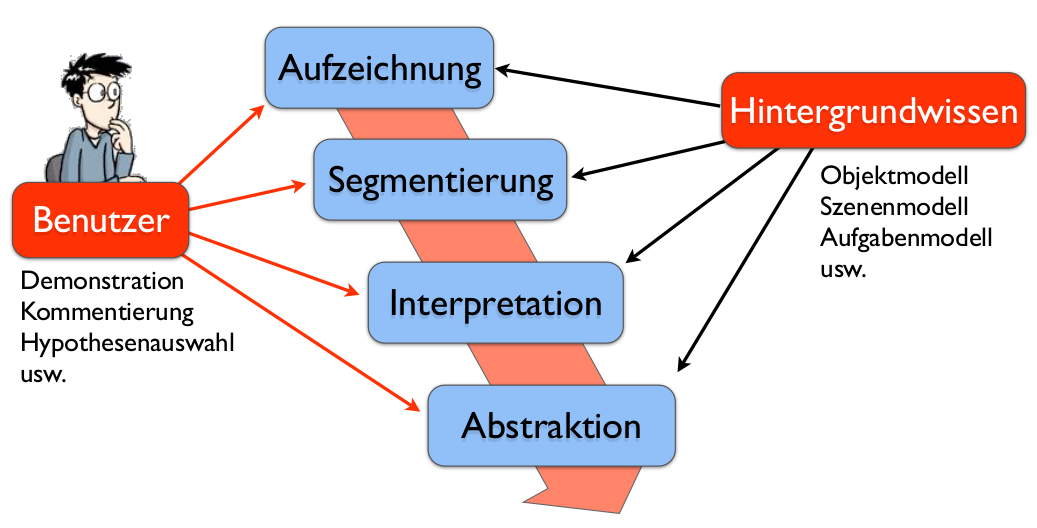
\includegraphics[width=0.6\linewidth]{figures/ch03_verarbeitungsschritte.png}
\caption{Lernsystem: Verarbeitungsschritte}
\label{fig:ch03_verarb}
\end{figure}

Abbildung \ref{fig:ch03_verarb} zeigt die Berarbeitungsschritte eines interaktiven Programmiersystems
%F18 ??
\subsubsection*{Ausführende Manipulatoren}
Ein Manipulator ist ein Roboter, der sich aus einer Steuerung und mechanischen Komponenten (Manipulatorarm) zusammen setzt. Er ist in der Lage, die Position und Orientierung
eines Objektes bezüglich eines Bezugskoordinatensystems zu ändern.
Es sind zwei Arten der Wissensrepräsentation zu unterscheiden, wie in Tabelle \ref{tab:Wissrep} dargestellt.

\begin{table}[hbt]
\centering
\begin{tabular}{|p{8cm}|p{8cm}|}
\hline
Manipulatorabhängige Repräsentation: \newline \textcolor{red}{subsymbolisch} & Manipulatorunabhängige Repräsentation: \newline \textcolor{red}{symbolisch}\\
\hline
Angabe von
\vspace{-4mm}
\begin{itemize}
\setlength\itemsep{0em}
\item Aktionssequenz oder
\item Gelenkwinkel-, Kraft und Momenttrajektorien
\end{itemize}
Nachteile: 
\begin{itemize}
\setlength\itemsep{0em}
\item[-] bei Serviceanwendungen nicht flexibel genug, da invariante Trajektorien keine Veränderung der Lage zu den manipulierten
Objekten in der Umwelt erlauben
\item[-] Variationen in Material, Form und Gewicht beim Manipulationsobjekt können nicht berücksichtigt werden; statische Trajektorien verlieren bei einer Veränderung dieser Werte zur
Programmausführung ihre Gültigkeit
\item[-] unterschiedliche Manipulatoren weisen aufgrund der Kinematik der Manipulatorarme und Endeffektoren verschiedene Konfigurationsräume auf und besitzenverschiedene Sensorausstattung
\item[-] bei expliziter Trajektorienerfassung benötigt man viel Speicher
\item[$\rightarrow$] durch die schwach strukturierte Umwelt und die Forderung von Wiederverwendbarkeit im Dienstleistungsbereich ist die manipulatorabhängige Repräsentation hier nicht sinnvoll
\end{itemize}
 &
 Angabe von Sequenzen von Elementaroperatoren
 \vspace{-4mm}
\begin{itemize}
\setlength\itemsep{0em}
\item Elementaroperatoren sind Regelungen mit Start-, End- und Fehlerkriterien
\item Implementierung der Elementaroperatoren ist manipulatorunabhängig
\item Effekte in der Umwelt sind manipulatorunabhängig, Situation wird nur über lokale Sensorwerte erstellte Umweltinformation beschrieben
\end{itemize}
Bewertung:
\begin{itemize}
\setlength\itemsep{0em}
\item[+] flexible Repräsentation und benutzerfreundliche symbolische Darstellung
\item[+] größere Flexibilität gegenüber Umweltveränderungen und unterschiedlichen Manipulatortypen
\item[+] Elementarfunktionen haben einen hohen Wiederverwendbarkeitswert, so braucht ein Programm nur die Sequenz der Elementarfähigkeiten
enthalten und ihre einzelnen Parameter bestimmen und repräsentieren;  oft weichen in einer
dynamischen Welt die Parameter der Elementarfähigkeiten von denen der Benutzerdemonstation ab, daher werden für variable Parameter Berechnungsfunktionen und
Auswahlbedingungen statt konkreter Werte benutzt
\item[-] Elementarfähigkeiten müssen für jeden Manipulator a-priori erzeugt werden 
\end{itemize}\\
\hline
\end{tabular}
\caption{Arten der Wissenrepräsentation}
\label{tab:Wissrep}
\end{table}

%Tabelle 5.1 Skript!!
\subsection{Wissensrepräsentation: Beispielsysteme}
\subsubsection*{Probabilistisch (Calinon \& Billard)}\footnote{[Calinon07]: What is the teacher’s role in robot programming by demonstration?\\
On learning, representing and generalizing a task in a humanoid robot}
Ziel: Lernen von Skills, z.B. Schachfigur bewegen
\begin{itemize}
\item Aktive, physische Demonstration am Roboter $\rightarrow$ kein Korrespondenzproblem
\item Repräsentation durch Gaussian Mixture Models (GMM) $\rightarrow$ subsymbolisch
\item Direkte Ausführung
\end{itemize}
Hierbei werden folgende Lerndaten benötigt:
\begin{itemize}
\item $(\theta, x, y, h)$: $n$ Demonstrationen mit je $T$ Trajektoriepunkten
\item $\theta$: Gelenkwinkel des Roboters + Zeitstempel
\item $x$: Kartesische Position der Hände + Zeitstempel
\item $y$: Distanzvektor der Hände zur Startposition des Objekts + Zeitstempel
\item $h$: Binärer Zustand des Greifers (offen, geschlossen) + Zeitstempel
\end{itemize}
Das Lernverfahren besteht dann aus folgenden Schritten: 
\begin{itemize}
\item Dimensionsreduktion und zeitliche Angleichung: $(\theta, x, y, h) \rightarrow (\theta^\prime, x^\prime, y^\prime, h^\prime)$
\item Lernen eines GMMs (vgl. Abbildung \ref{fig:ch03_gmm}) für alle Komponenten, z.B. $x^\prime$ (4-dimensional) mit Dichte $p(x^\prime)$:
\begin{align*}
p(x^\prime) = \sum\limits_{i=1}^k p(i)p(x^\prime|i) = \sum\limits_{i=1}^k \pi_i \mathcal{N}(x^\prime; \mu_i, \Sigma_i)
\end{align*} mit $k$ = Anzahl der Normalverteilungen, $\pi$ = Gewichtung, $\mathcal{N}$ = Normalverteilung
\item Bestimmung von $k$: Bayes‘sches Informationskriterium und EM-Algorithmus
\begin{figure}[ht]\centering 
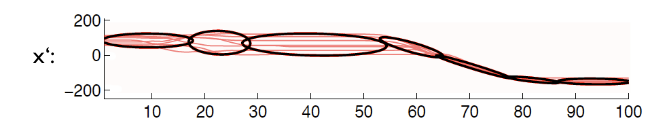
\includegraphics[width=0.6\linewidth]{figures/ch03_gmm.png}
\caption{Gaussian Mixture Model}
\label{fig:ch03_gmm}
\end{figure}
\end{itemize}
Die Repräsentation gestaltet sich folgendermaßen:
\begin{itemize}
\item Probabilistische Darstellung der Trajektorien $x^\prime: t \mapsto \mathcal{N}(\mu_{x^\prime}(t), \Sigma_x(t))$
\item Berechnung durch Gaussian Mixture Regression (vgl. Abbildung \ref{fig:ch03_gmr}): Gewichtung der bedingten Wahrscheinlichkeiten $p(x^\prime, i|t)$
\begin{align*}
\mu_{x^\prime}(t) = \sum\limits_{i=1}^k \beta_i(t)\mu_{i, x^\prime|t} \text{ und } \Sigma_{x^\prime}(t) = \sum\limits_{i=1}^k \beta_i(t)^2\Sigma_{i, x^\prime|t}\\
\text{ mit } p(x^\prime,i|t) = \mathcal{N}(\mu_{i, x^\prime|t}, \Sigma_{i, x^\prime|t}) \text{ und } \beta_i(t) = \frac{p(t|i)}{\Sigma{j=1}^k p(t|j)}
\end{align*}
\begin{figure}[ht]\centering 
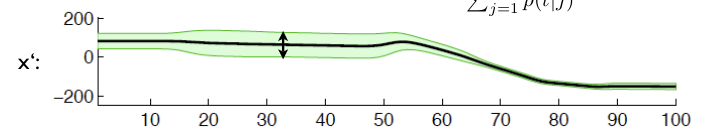
\includegraphics[width=0.6\linewidth]{figures/ch03_gmr.png}
\caption{Gaussian Mixture Regression}
\label{fig:ch03_gmr}
\end{figure}
\end{itemize}
Die Ausführung besteht dann aus folgenden Schritten:
\begin{itemize}
\item Definition eines quadratischen Ähnlichkeitsmaßes: \Gu metric of imitation\Go
\item Gewichtung der Abweichung von den Mittelwerten in $t$, z.B. $\mu_{x^\prime}(t)$
\item Wahl der Gewichtsmatrix: $(\Sigma_{x^\prime}(t))^{-1}$
\item Bestimmung des Nachfolgerzustands $\theta(t+1)$ bzw. der Transition $\theta(t) \rightarrow \theta(t+1)$, die
das Ähnlichkeitsmaß minimiert
\item Jacobi-Matrix zur Kombination von kartesischen und Gelenkwinkeleinschränkungen
\end{itemize}
Eine Bewertung des Verfahrens ist in Tabelle \ref{tab:cabi} dargestellt.
\begin{table}[hbt]
\centering
\begin{tabular}{|p{6.5cm}|p{6.5cm}|}
\hline
Vorteile & Nachteile\\
\hline
\vspace{-5mm}
\begin{itemize}
\setlength\itemsep{0em}
\item[+] schnelles Verfahren, ähnlich Playbackprogrammierung
\item[+] automatische Adaptierung an Änderungen der Objektpositionen
\end{itemize}
 &
 \vspace{-5mm}
\begin{itemize}
\setlength\itemsep{0em}
\item[-] relevante Merkmale manuell definiert, hier z.B. nur Distanz zu Startposition
\item[-] geringe Generalisierung, da keine Vorbedingungen, Ziele, Kollisionen
 keine zielgerichtete Erzeugung von Bewegungen
\item[-] keine Validierung
\end{itemize}\\
\hline
\end{tabular}
\caption{Zusammenfassung: Calinon, Billard}
\label{tab:cabi}
\end{table}\\ 
\subsubsection*{Dynamisch (Pastor \& Schaal)\footnote{[Pastor09]: Learning and generalization of motor skills by learning from demonstration}}
Ziel: Lernen von Skills, z.B. Tennisschwung
\begin{itemize}
\item Aktive, physische Demonstration am Roboter $\rightarrow$ kein Korrespondenzproblem
\item Repräsentation durch Dynamic Movement Primitives (Differentialgleichungen)
\item Direkte Ausführung
\end{itemize}
Die Repräsentation ist wie folgt:
\begin{itemize}
\item Implizite Darstellung durch Menge von Differentialgleichungen:
\begin{align*}
\tau \dot{v} &= K(g-x) -Dv + (g-x_0)f\\
\tau \dot{x} &= v\\
\end{align*}
\item $x$ = Position, $v$ = Geschwindigkeit, $K$ = Federkonstante,
$D$ = Dämpfung, $g$ = Ziel, $x_0$ = Start, $\tau$ = zeitliche Skalierung
\item $f$ = nicht-lineare Funktion, die die Demonstrationsmenge approximiert:
\begin{align*}
f(s) = \frac{\sum_{i=1}^n w_i\psi_i(s)s}{\sum_{i=1}^n \psi_i(s)} \text{ mit } \tau \dot{s} = -\alpha s
\end{align*}
\item Vorteil: Gewichte hängen nicht von $\tau, x_0 $ und $g$ ab
\ita Änderungen von Start, Ziel und der zeitlichen Skalierung möglich
\ita Generalisierung eingeschränkt möglich
\end{itemize}
Das Lernen läuft in folgenden Schritten ab:
\begin{itemize}
\item Berechnung von $v(t), \dot{v}(t)$ für jede Demonstration $x(t)$
\item $s(t)$ wird durch Integration berechnet
\item Der Wert $f(s)$ wird berechnet
\item $\psi_i$ sind nicht normalisierte Normalverteilungen (\Gu Gauss‘sche Basisfunktionen\Go)
\item Bestimmung der Parameter $w_i$ durch lineare Regression
\end{itemize}
Die Ausführung erfolgt über die Berechnung von $v(t), \dot{v}(t)$ im aktuellen Zustand und Integration.\\
Eine Bewertung des Verfahrens ist in Tabelle \ref{tab:pascha} dargestellt.
\begin{table}[hbt]
\centering
\begin{tabular}{|p{6.5cm}|p{6.5cm}|}
\hline
Vorteile & Nachteile\\
\hline
\vspace{-5mm}
\begin{itemize}
\setlength\itemsep{0em}
\item[+] schnelles Verfahren
\item[+] automatische Adaptierung an Start und Ziel
\item[+] lokale Hindernisvermeidung möglich
\end{itemize}
 &
 \vspace{-5mm}
\begin{itemize}
\setlength\itemsep{0em}
\item[-] relevante Merkmale manuell definiert
\item[-] geringe Generalisierung
\item[-] keine Validierung
\end{itemize}\\
\hline
\end{tabular}
\caption{Zusammenfassung: Pastor, Schaal}
\label{tab:pascha}
\end{table}\\ 
\subsubsection*{Sub-/Symbolisch (IPoR II)}
IPor (Interaktives Programmieren von Robotern wurde an der Universität Karlsruhe entwickelt. \\
Problembeschreibung:
\begin{itemize}
\item Robotersystem mit sehr vielen Freiheitsgraden (Kuka LBR / SAH/HIT: 40)
\item  Fingerfertige Manipulation fester Körper („rigid bodies“)
\item Roboterarbeitsraum in realen Situationen stark eingeschränkt (z.B.
Kollisionen)
\item  \Gu Korrespondenzproblem\Go: Mensch und Roboter haben unterschiedliche
Kinematik, d.h. keine direkte Abbildung menschlicher Bewegungen möglich
\end{itemize}
Einsatz von Planungsmethoden:
\begin{itemize}
\item Repräsentation der Manipulationsaufgabe als Bahnplanungsproblem mit Einschränkungen
\item Autonome Planung von Bewegungen, die das Ziel einer Manipulationsaufgabe erfüllen
\item Problem: Manuelle Definition des Planungsproblems ist komplex (z.B. $\leq$ 40 dofs)
\ita Lernen von Planungsproblemen aus der Beobachtung des Menschen
\end{itemize}
Repräsentation als Bahnplanungsproblem mit Einschränkungen:
\begin{itemize}
\item Beschränkung der Bewegung eines Koordinatensystems relativ zu einem zweiten Koordinatensystem (ähnlich \Gu Task Frames\Go) 
\item Drei Typen von Bewegungseinschränkungen:
\begin{itemize}
\item Positionseinschränkungen
\item Orientierungseinschränkungen
\item Richtungseinschränkungen
\end{itemize}
\item Definition: Eine Einschränkung ist ein 5-Tupel $(t, f, M, g, R)$ mit
\begin{itemize}
\item Typ $t$
\item Koordinatensystemen $f, g$
\item homogener Transfromationsmatrix $M$, relativ zu $f$
\item Region $R$
\end{itemize}
%Wiederholungsfolien 35, 36 ausgelassen
\item Wann ist eine Einschränkung erfüllt?
\begin{itemize}
\item Transformation von $M$ definiert in $f$ relativ zu $g$:
\begin{align*}
M^\prime &= ^0H_g^{-1} \cdot ^0 H_f \cdot M\\
M^\prime &= ^g H_f \cdot M
\end{align*}
\item Umwandlung von $M^\prime$ in 3d-Vektor $m^\prime$:\\
$t$ = Position, Richtung: $m^\prime = (x y z)$\\
$t$ = Orientierung: $m^\prime = (r_x r_y r_z )$
\item Bestimmung des nächsten Punkts $n$ in $R$ und der Distanz $d = | m^\prime - n |$
\item Erfüllt, wenn $d < \varepsilon$
\end{itemize}
\item Repräsentation des Planungsproblems als \Gu Strategiegraph\Go :
Tupel $X, C^t_n, C^t_e, C^b_n, C^b_e)$ mit Knoten $X$, zeitliche Einschränkungen der Knoten $C^t_n$ und Kanten $C^t_e$,
Bewegungseinschränkungen der Knoten $C^b_n$ und Kanten $C^b_e$
\end{itemize}
Abbildung \ref{fig:ch03_stratgra} zeigt ein Beispiel eines solchen Graphen.
\begin{figure}[ht]\centering 
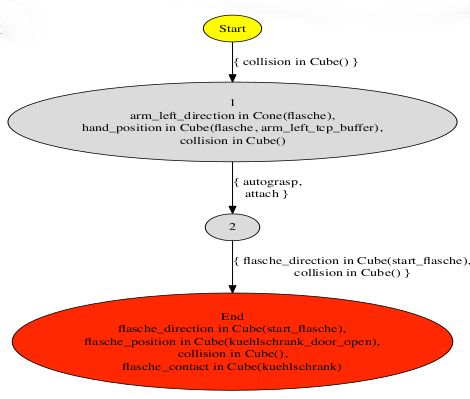
\includegraphics[width=0.6\linewidth]{figures/ch03_strategiegraph.png}
\caption{Beispiel eines Strategiegraphen: \Gu Einschenken\Go $\rightarrow$ Die Ausführungsumgebung bezieht sich auf Unterschiede in Objekten,
Objektposen und Hindernissen (verglichen mit Demonstrationen). Einschränkungen im Strategiegraphen referenzieren Koordinatensysteme. Deren Lage wird automatisch adaptiert. Bei Ausführung unter Verwendung von Bahnplanung repräsentieren die Knoten des Graphen Teilziele der Manipulationsaufgabe, seine Kanten Übergänge zwischen den Teilzielen. Ein Planungsproblems wird für jedes Teilziel gelöst.}
\label{fig:ch03_stratgra}
\end{figure}

\noindent
Im Folgenden soll der PdV-Zyklus (vgl. Abbildung \ref{fig:ch03_zykl}) beispielhaft an IPoR II 
verdeutlicht werden. %Hierzu viele potentiell relevante Bilder auf den Folien 
\paragraph*{Beobachtung} Als Sensorik wird verwendet: Mikrofon, Deckenkameras, Stereokamera mit Pan-Tilt-Unit, Flock-of-Birds, Voodoo, Cybergloves\\
Virtual Technology - Datenhandschuh, Meßprinzip: Dehnmessstreifen, 20 Fingerbeugungs- und Spreizwinkel + 2 Freiheitsgrade im Handgelenk\\
Bestimmung der Position und Orientierung der menschlichen Hände sowie von Objekten: Magnetfeldbasierter Positionstracker, Stereokamera

\paragraph*{Segmentierung}
\begin{itemize}
\item Ziel (mit Interpretationsphase): Repräsentation der demonstrierten Handlung durch Sequenz von zu
erfüllenden Teilzielen (= Topologie des Strategiegraphs)
\item Ansatz: schwellwertbasierte Segmentierung zur Bestimmung von markanten Zeitpunkten der Demonstration
\item Vorteile: einfache Interaktionsmöglichkeit während der Demonstration, einfache Korrektur von Hypothesen
\item Erzeugung eines Segmentierungspunkt, wenn Hand-, Fingergeschwindigkeit gering ist und mindestens ein Finger Objektkontakt % vgl Skript, IPor 1 !!
hat
\end{itemize}

\paragraph*{Interpretation} 
\begin{itemize}
\item Klassifikation der Segmentierungspunkte in 4 Typen auf Basis des Weltzustands an den Intervallgrenzen: 
\begin{itemize}
\item Kein Objekt
\item Objekt aufgenommen
\item Objekt gehalten
\item Objekt losgelassen
\end{itemize}
\item Lernen des Planungsmodells
\begin{itemize}
\item  Topologie des Strategiegraphs: Segmentierung der Bewegungen des linken und rechten Arms, Kombination zu einem Graphen (vgl. \autoref{sg})
\item Erzeugung der Bewegungseinschränkungen: Manuell definierte Koordinatensysteme für alle Objekte: $K = \{ \text{Flaschenöffnung, Becheröffnung,
Rechter Zeigefinger, Welt, ...} \}$; Erzeugung aller möglichen Einschränkungen $(t, f, M, g, R)$ mit $f,g \in K$, Typ $t$ beliebig,
für jeden Knoten und jede Kante $\rightarrow$ Region $R$ muss bestimmt werden (vgl. \autoref{sg1})
\item Beispiel: $f$ = Flaschenöffnung, $g$ = Welt, $t$ = Richtung; $f$ = Flaschenöffnung, $g$ = Becheröffnung, $t$ = Position
\end{itemize}
\begin{figure}[h!]
	\centering
	\begin{subfigure}{.4\textwidth}
		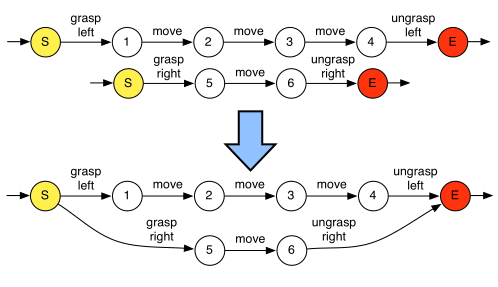
\includegraphics[width=\textwidth]{figures/ch03_stratgraph.png}
		\caption{}
		\label{sg}
	\end{subfigure}
	\begin{subfigure}{.4\textwidth}
		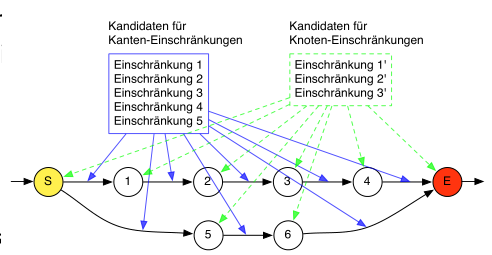
\includegraphics[width=\textwidth]{figures/ch03_stratgraph1.png}
		\caption{}
		\label{sg1}
	\end{subfigure}
	\caption{}
\end{figure}
\item Bestimmung der Region $R$: Für jede Einschränkung $(t, f, M, g, R)$
\begin{itemize}
\item Bestimmung des Werts von $f$ in jedem Punkt $t_i$ des Segments: $g^H_f(t_i) \cdot M$
\item Umwandlung in 3d-Vektor $m^\prime(t_i)$
\item Ergebnis: Menge von 3d-Vektoren
\item Bestimme Region $R$, die alle 3d-Vektoren einschließt
\ita Beispiel: Knoten-Einschränkung ($f$ = Flaschenöffnung, $g$ = Becheröffnung, $t$ = Position)
\end{itemize}
\end{itemize}
\paragraph*{Abstraktion}
Ziel: Anwendbarkeit des Planungsmodells in neuen Situationen auf verschiedenen Robotern
\begin{itemize}
\item Weitere Einschränkungen: Kräfte, Kontakte, Objektbewegung
\item Wesentliche Abstraktion durch Koordinatensysteme und Einschränkungen
\ita Abbildung von objektabhängigen Koordinatensystemen, \\z.B. Flasche.Öffnung $\rightarrow$ Milchpackung.Öffnung
\end{itemize} 

\paragraph*{Ausführung}
\begin{itemize}
\item Gelernte Einschränkungen definieren Suchraum für Roboterbewegungen
\item Einsatz von \textit{Bahnplanung unter Einschränkungen} zur Ausführung von gelernten
Planungsmodellen
\item Einsatz von \textit{Griffplanung} zur Bestimmung qualitativ hochwertiger Griffe
\end{itemize}
Eine Bewertung des Verfahrens ist in Tabelle \ref{tab:ipo} dargestellt.
\begin{table}[hbt]
\centering
\begin{tabular}{|p{6.5cm}|p{6.5cm}|}
\hline
Vorteile & Nachteile\\
\hline
\vspace{-5mm}
\begin{itemize}
\setlength\itemsep{0em}
\item[+] Generalisierung auf Basis von Objekteigenschaften
\item[+] Start- und Zielbeschreibung, Validierbarkeit
\item[+] Hindernisvermeidung und Berücksichtigung von Einschränkungen
\item[+] mehrere Lösungen und beliebige Optimalitätskriterien
\end{itemize}
 &
 \vspace{-5mm}
\begin{itemize}
\setlength\itemsep{0em}
\item[-] hoher Aufwand (Planungszeit, Simulationszeit)
\item[-] 3d-Modelle der Objekte, menschlichen Hand notwendig
\item[-] automatische Segmentierung bei dynamischen Bewegungen schwierig
\end{itemize}\\
\hline
\end{tabular}
\caption{Zusammenfassung: IPOR II}
\label{tab:ipo}
\end{table}\\ 
%Nächste VL:
%• Bahnplanung
%• Grifftaxonomie
%• Griffplanung
\subsection{Bahnplanung}
Zunächst einige relevante Definitionen:
\begin{itemize}
\item \red{Konfiguration $K$}: vollständige, eindeutige Beschreibung
des Zustands eines Roboters $A$, z.B.
\begin{itemize}
\item im euklidischen Raum durch seine Position und Orientierung
\item im Gelenkwinkelzustandsraum durch die Werte der Gelenke
\end{itemize}
\item \red{Konfigurationsraum $\mathbb{K}$}: Raum aller
möglichen Konfigurationen des Roboters $A$
\item \red{Weg} des Roboter $A$ von der Konfiguration $K_{Start}$ zu $K_{Ziel}$ ist eine stetige Abbildung:
\begin{align*}
\tau: [0, 1] \rightarrow \mathbb{K}\\
\tau(0) = K_{Start} ,\tau(1) = K_{Ziel}
\end{align*}
\item \red{Einschränkung} für den Roboter $A$ ist eine Abbildung:
\begin{align*}
\lambda : \mathbb{K} \rightarrow [0, 1]
\end{align*} 
\item \red{Arbeitsraumhindernis $H$}: Raum, welcher von
einem Objekt im Arbeitsraum eingenommen wird
\item \red{Konfigurationsraumhindernis $\mathbb{K}_{H_i}$}: Menge aller
Punkte des Konfigurationraumes, welche innerhalb eines
Arbeitsraumhindernisses $H_i$ liegen:
\begin{align*}
\mathbb{K}_{H_i} = {K \in \mathbb{K} | K \in H_i}
\end{align*}
\item \red{Hindernisraum $\mathbb{K}_{H_i}$}: Menge aller
Konfigurationsraumhindernisse:
\begin{align*}
\mathbb{K}_H =\bigcup_i \mathbb{K}_{H_i}
\end{align*}
\item \red{Freiraum $\mathbb{K}_F$}: Menge aller Punkte aus $\mathbb{K}$, welche nicht im
Hindernisraum liegen:
\begin{align*}
\mathbb{K}_F = \mathbb{K}\backslash \mathbb{K}_H
\end{align*}
\item \red{kollisionsfreier Weg $\tau$}: Weg mit $Bild(\tau) \subseteq \mathbb{K}_F$, also ein Pfad welcher alle Einschränkungen erfüllt
\end{itemize}
Bei einer Bahnplanung im Konfigurationsraum werden Bewegungen eines Roboters als \red{Trajektorie im Konfigurationsraum}, d.h. als Zustandsänderungen über die Zeit
relativ zu einem stationären Koordinatensystem (kartesischer Raum, Gelenkwinkelraum) aufgefasst:
\begin{itemize}
\item Gegeben: $K_{Start}$ = Startkonfiguration, $\land_{Ziel}$ = Menge der Zieleinschränkungen
\item Gesucht: Kollisionsfreier Weg $\tau$ von $K_{Start}$ nach $K$ mit $\lambda(K)=1 \forall \lambda \in \land_{Ziel}$
\item Bedingungen: i.A. Gütekriterien, Neben-,Rand- sowie Zwangsbedingungen
\end{itemize}
Hierbei sei angemerkt, dass von Roboter und Umwelt zu einem Punkt im Konfigurationsraum abstrahiert wird. Die Kollisions- bzw. Einschränkungsüberprüfung stellt eine Blackbox
\begin{align*}
f: \mathbb{K} \rightarrow \{0, 1\}\\
\text{Beispiel:} f(K) = \bigwedge\limits_{\varv \in \land_{Weg}}^{} \varv(K) \geq \varepsilon(\varv)
\end{align*}
dar. Bei Entwicklung allgemeiner Planungsverfahren auf Basis dieser Abstraktion entspricht die Bahnplanung einer Suche nach einer stetigen Verbindung zweier Punkte im
Konfigurationsraum. Eine explizite Beschreibung des Freiraums ist nicht notwendig, d.h. das Suchverfahren ist unabhängig von der Struktur und Repräsentation des Freiraums.

\subsubsection*{Simpler Rapidly-exploring Random Tree (RRT) Planer}
\paragraph*{RRT-Algorithmus}
Wie bereits zu Anfang des Kapitels erwähnt, bringt die humanoide Servicerobotik zahlreiche Anforderungen mit sich, sowie die Manipulation beliebiger Objekte, das selbstständige Lösen komplexer Aufgaben und den Einsatz im menschlichen Umfeld, d.h. humanoide Serviceroboter müssen in einer sehr komplexen Umgebung agieren und verfügen über sehr viele Freiheitsgrade (der Roboter Albert II beispielsweise hat 13df,  6 im Arm, 3 in der Plattform und 4 in der Hand. Daraus ergibt sich ein 13-dimensionaler Konfigurationsraum $\mathbb{R}^{13}$ als reellwertige Grundlage).
Ein Bahnplanungsalgorithmus, der hiermit umgehen kann ist der RRT = Rapidly-exploring Random Tree\footnote{[LaValle/Kuffner99]: Randomized Kinodynamic
Planning}, welcher zur effizienten Durchsuchung hoch-dimensionaler Räume entwickelt wurde. Er ist geeignet für holonome und nicht-holonome Problemstellungen mit Einschränkungen. Es wird inkrementell eine Baumstruktur aufgebaut und dabei der erwartete Abstand eines Punkts zu einem Knoten im Baum minimiert. Wenn die Zeit $t$ gegen unendlich geht kommt man beliebig nah an jeden beliebigen Punkt. Der Algorithmus erreicht eine hohe Geschwindigkeit durch schnelles Wachstum in nicht explorierte Bereiche. Die Wurzel ist ein Punkt im 13-dimensionalen Konfigurationsraum. Pseudocode ist in Algorithmus \ref{alg:rrt}. 
Eine graphische Veranschaulichung zeigt \autoref{fig:rrt}.
Der Knoten mit der größten Voronoi-Region hat jeweils die größte Wahrscheinlichkeit, als nächstes erweitert zu werden (\textbf{Voronoi-Bias}). Da am Anfang die Voronoi-Gebiete am
Randbereich groß sind findet zunächst eine rasche Exploration und dann eine Verfeinerung statt (vgl. Abbildungen \ref{fig:vb} und \ref{fig:vb1}).
\begin{algorithm}
  \caption{RRT
    \label{alg:rrt}}
  \begin{algorithmic}[1]
    %\Require{$x$ and $y$ are packed \DNA strings of equal length $n$}
    %\Statex
    \Statex {BUILD\_RRT}($K_{Start}, n, \varepsilon$)
      \State $T$.init($K_{Start}$) \Comment{Neuer Baum mit Startkonfiguration in der Wurzel}
      \For{$k = 1 \textrm{ to } n$}
        \Let{$K_{Zuf}$}{RAND\_CONF()} \Comment{Gleichverteilt zufällige Erzeugung einer Konfiguration}
        \Let{$K_{Nahe}$}{NEAREST\_VERTEX($K_{Zuf}, T$)} \Comment{Bestimmung des nächsten Knotens}
        \Let{$K_{Neu}$}{EXTEND($K_{Nahe}, K_{Zuf}, \varepsilon$)} \Comment{Erzeugung einer neuen Konfiguration}
        \State $T$.add\_vertex($K_{Neu}$)
        \State $T$.add\_edge($K_{Nahe}, K_{Neu}$)
      \EndFor
      \State \Return{$T$}
    %\EndFunction
  \end{algorithmic}
\end{algorithm}

%Beispiel für Verwendung des Algorithmus-Packages
%\begin{algorithm}
%  \caption{Counting mismatches between two packed \DNA strings
%    \label{alg:packed-dna-hamming}}
%  \begin{algorithmic}[1]
%    \Require{$x$ and $y$ are packed \DNA strings of equal length $n$}
%    \Statex
%    \Function{Distance}{$x, y$}
%      \Let{$z$}{$x \oplus y$} \Comment{$\oplus$: bitwise exclusive-or}
%      \Let{$\delta$}{$0$}
%      \For{$i \gets 1 \textrm{ to } n$}
%        \If{$z_i \neq 0$}
%          \Let{$\delta$}{$\delta + 1$}
%        \EndIf
%      \EndFor
%      \State \Return{$\delta$}
%    \EndFunction
%  \end{algorithmic}
%\end{algorithm}
\begin{figure}[h!]
	\centering
	\begin{subfigure}{.4\textwidth}
		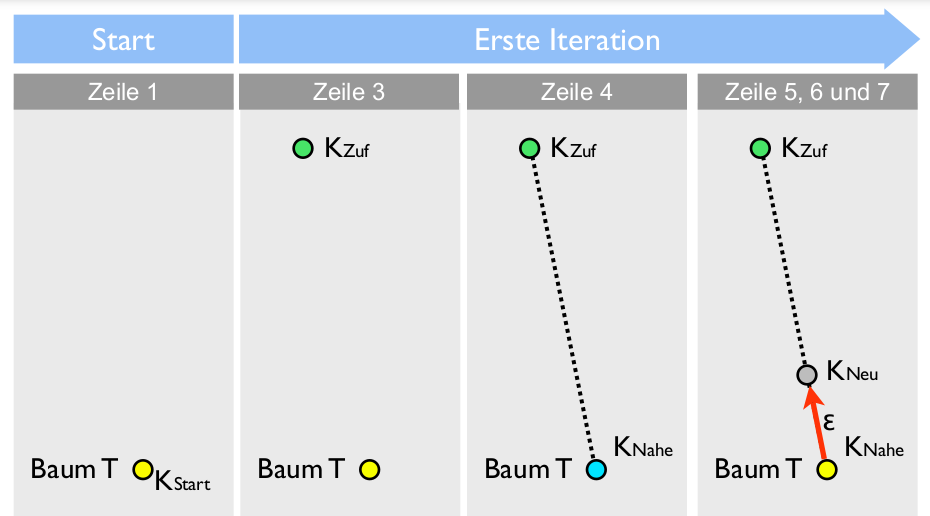
\includegraphics[width=\textwidth]{figures/ch04_rrt1.png}
	\end{subfigure}
	\begin{subfigure}{.4\textwidth}
		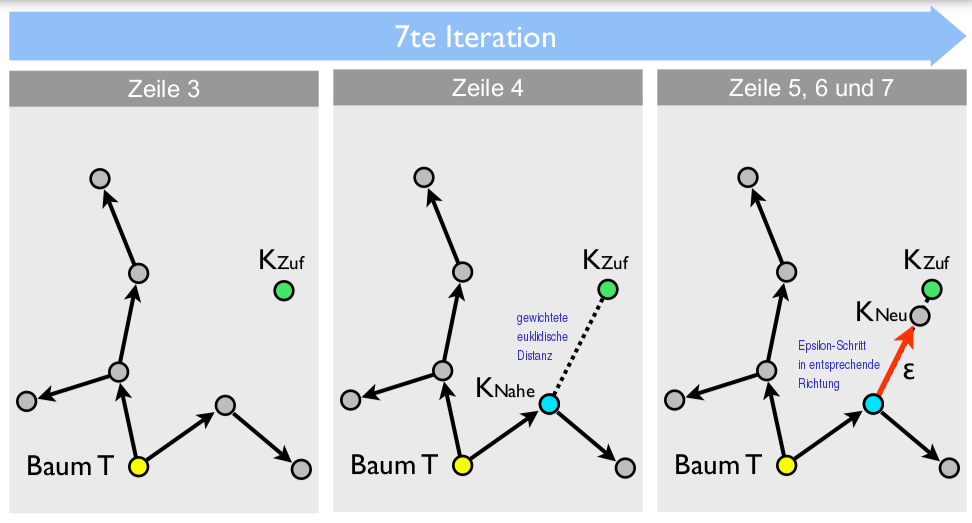
\includegraphics[width=\textwidth]{figures/ch04_rrt2.png}
	\end{subfigure}
	\caption{Graphische Veranschaulichung - RRT}
	\label{fig:rrt}
\end{figure}
\begin{figure}[h!]
	\centering
	\includegraphics[width=.3\textwidth]{figures/ch04_voronoi.png}
	\caption{Voronoi-Bias -- Detail}
	\label{fig:vb}
\end{figure}
\begin{figure}[h!]
	\centering
	\begin{subfigure}{.3\textwidth}
		\includegraphics[width=\textwidth]{figures/ch04_voron1.png}
	\end{subfigure}
	\begin{subfigure}{.3\textwidth}
		\includegraphics[width=\textwidth]{figures/ch04_voron2.png}
	\end{subfigure}
	\begin{subfigure}{.3\textwidth}
		\includegraphics[width=\textwidth]{figures/ch04_voron3.png}
	\end{subfigure}
	\begin{subfigure}{.3\textwidth}
		\includegraphics[width=\textwidth]{figures/ch04_voron3.png}
	\end{subfigure}
	\begin{subfigure}{.3\textwidth}
		\includegraphics[width=\textwidth]{figures/ch04_voron5.png}
	\end{subfigure}
	\begin{subfigure}{.3\textwidth}
		\includegraphics[width=\textwidth]{figures/ch04_voron6.png}
	\end{subfigure}
	\caption{Voronoi-Bias}
	\label{fig:vb1}
\end{figure}
RRT: Zusammenfassung
\begin{itemize}
\item Allgemeines Verfahren zur Durchsuchung hoch-dim. Räume
\item Online-Verfahren
\item Approximation des Suchraums durch eindimensionale Struktur: Baum
\item Rasche Exploration des Suchraums: Voronoi-Bias
\item Probabilistische (oder deterministische) Stichprobenerzeugung
\item Einfach zu implementieren, nur wenige Parameter ($\varepsilon$, Distanzfunktion auf $\mathbb{K}$)
\end{itemize}
\paragraph{Anwendung in der Bahnplanung} Es sind drei Fragen zu klären:
\begin{enumerate}
\item Wie Einschränkungen berücksichtigen?
\item Wie zielgerichtet suchen?
\item Wie kollisionsfreie Wege erzeugen?
\end{enumerate}
Hierzu muss der Basisalgorithmus erweitert werden:
\begin{itemize}
\item Es werden nur Konfigurationen hinzugefügt, die alle Einschränkungen erfüllen.
\item Bei der Stichprobenerzeugung werden mit einer bestimmten Wahrscheinlichkeit Zielkonfigurationen generiert, der Baum wächst in die Richtung der Zielkonfigurationen.
\item Der Planungsprozess ist beendet, wenn die letzte Konfiguration die Zieleinschränkungen erfüllt.
\end{itemize} 
\textbf{Frage 1 \& 2: Einbeziehung von Einschränkungen und Umgang mit Kollisionen} (vgl. \autoref{fig:einschr})
\begin{itemize}
\item $K_{Neu}$ wird übernommen, wenn alle Einschränkungen zwischen $K_{Nahe}$ nach $K_{Neu}$ erfüllt sind
\item Keine Distanz, nur Ja / Nein
\item Kollisionen auf Grundlage eines Geometriemodells der Objekte (Standard: 3D-Dreiecksnetze)
\item Kollisionsüberprüfung: mindestens zwei Dreiecke schneiden sich (oder 1. Objekt in 2. komplett enthalten)
\item hierzu gibt es optimierte Algorithmen, ist vergleichsweise langsam
\end{itemize}
\begin{figure}[h!]
	\centering
	\begin{subfigure}{.3\textwidth}
		\includegraphics[width=\textwidth]{figures/ch04_Kol.png}
		\caption{$K_{Zuf}$ könnte auch schon ZK erfüllen, überprüfe dies, falls ja ist Planung beendet}
		\label{kol}
	\end{subfigure}
	\begin{subfigure}{.5\textwidth}
		\includegraphics[width=\textwidth]{figures/ch04_Kol1.png}
		\caption{Der Roboter \glqq weiß\grqq{} um das Vorhandensein des Tisches nur über Einschränkungen; es wird der Schnitt zweier Dreiecke berechnet; da hier der Teller im Tisch hängt wird diese Konfiguration dem Baum nicht hinzugefügt}
	\end{subfigure}
	\caption{Einbeziehung von Einschränkungen und Kollisionen}
	\label{fig:einschr}
\end{figure}
\textbf{Frage 3: Wie zielgerichtet planen?}
Wie in \autoref{vb1} dargestellt definiert die Menge der Zieleinschränkungen i.d.R. ein stark begrenztes Gebiet in $\mathbb{K}$ (roter Bereich im 6. Panel der Abbildung), z.B. endliche Menge von gültigen Zielkonfigurationen. Somit ist die Wahrscheinlichkeit eine Zielkonfiguration zufällig zu erzeugen minimal, es dauert recht lange bis der Baum in den betreffenden Bereich reinwächst.
Daher ist die in Algorithmus \autoref{alg:rrt-detail} dargestellte Modifikation der Stichprobenerzeugung sinnvoll (vgl. \autoref{rrt-erw}).\\
\begin{algorithm}
  \caption{Detail
    \label{alg:rrt-detail}}
  \begin{algorithmic}[1]
    %\Require{$x$ and $y$ are packed \DNA strings of equal length $n$}
    %\Statex
    \Statex {RAND\_CONF}($f_{Ziel}, \delta$) \Comment{z.B. $\delta = 0.01$}
      \State $P \thicksim U(\left[0,1\right])$
      \If{$P < \delta$}
      	\State \Return{$K \in \mathbb{K}: f_{Ziel}(K) = 1$}
      \Else
      	\State \Return{$K \thicksim U(\mathbb{K})$}
      \EndIf
    %\EndFunction
  \end{algorithmic}
\end{algorithm}
\begin{figure}[h!]
	\centering
	\includegraphics[width=.5\textwidth]{figures/ch04_rrt-erw.png}
	\caption{Erweiterung -- Zielgerichtet planen mit RRT}
	\label{rrt-erw}
\end{figure}
\begin{algorithm}[h!]
  \caption{Simpler RRT Planer
    \label{alg:rrt-erw}}
  \begin{algorithmic}[1]
    \Statex {RRT\_SIMPLE}($K_{Start}, \textcolor{red}{f_{Ziel}}, \textcolor{red}{f_{Weg}}, \varepsilon, \textcolor{red}{\delta}$)
      \State $T$.init($K_{Start}$) \Comment{$f_{Ziel}$ ist Blackbox für Zieleinschränkungen}
      \For{$k = 1 \textrm{ to } MAX$}
        \Let{$\textcolor{red}{K_{Zuf}}$}{\textcolor{red}{RAND\_CONF($f_{Ziel}, \delta$)}} 
        \Let{$K_{Nahe}$}{NEAREST\_VERTEX($K_{Zuf}, T$)} \Comment{$f_{Weg}$ ist Blackbox für Einschränkungen}
        \Let{$K_{Neu}$}{EXTEND($K_{Nahe}, K_{Zuf}, \varepsilon$)} \Comment{Erzeugung einer neuen Konfiguration}
        \If{\textcolor{red}{$f_{Weg}(K_{Neu}) = 1$}}
        	\State $T$.add\_vertex($K_{Neu}$)
        	\State $T$.add\_edge($K_{Nahe}, K_{Neu}$)
        	\If{\textcolor{red}{$f_{Ziel}(K_{Neu}) = 1$}} \Comment{Lösungspfad: Rückverfolgung der Elternknoten beginnend mit dem letzten Knoten}
        		\State \Return{$T$, Gefunden}
        	\EndIf
        \EndIf
      \EndFor
      \State \Return{$T$, Nicht gefunden}
  \end{algorithmic}
\end{algorithm}
\bigskip
\textbf{Beispiel für die Anwendung des Simplen RRT Planers}: Holonome Planung für einen Roboterarm mit 7 Freiheitsgraden (vgl. \autoref{fig:rrt-bsp})
\begin{itemize}
\item Konfigurationsraum $\mathbb{K}= \left[0,1\right]$ (Gelenkwinkelbereich $\left[-170°, +170°\right]$ wird auf Bereich $\left[0,1\right]$ normiert)
\item Distanzfunktion auf $\mathbb{K}$: $d(k,s) = \sum\limits_{i = 1...7} w_i (k_i - s_i)$
\item Gewichtsvektor $w=(1.5,1.5,1.5,1.25,1,1,1)$
\item $\varepsilon = 0.001, \delta = 0.01$ (Schrittweite: mit welcher WK man Zielkonfiguration erzeugt)
\item $f_{Ziel}(K) = 1 \Leftrightarrow K = K_ {Ziel}$
\item $f_{Weg}(K) = 1 \Leftrightarrow K$ ist kollisionsfrei
\end{itemize}
\begin{figure}[h!]
	\centering
	\includegraphics[width=.5\textwidth]{figures/ch04_rrt-bsp.png}
	\caption{Beispiel für die Anwendung des Simplen RRT Planers: Arm bewegt sich relativ weich, auf recht glatter Bahn}
	\label{fig:rrt-bsp}
\end{figure}
\subsubsection*{Pfadglättung und Hinderniserweiterung}
\textbf{Reale Anwendung}: Der Planer kann so nicht direkt eingesetzt werden
\begin{itemize}
\item Glättung notwendig, da Weg nicht glatt
\item Hinderniserweiterung notwendig, da kleine Abweichungen von der Bahn zu Kollisionen führen können
\end{itemize}
\textbf{Verringerung der Länge des Lösungswegs} (siehe \autoref{fig:abkuerz}):
\begin{itemize}
\item Zufällige Wahl zweier Knoten im Lösungsweg
\item Überprüfung der Verbindung beider Knoten auf Einhaltung der Einschränkungen
\item Falls die Verbindung geringere Kosten aufweist als der entsprechende Teillösungspfad, Verbindung der beiden Knoten und Löschen der dazwischenliegenden Knoten aus dem Lösungspfad
\end{itemize}
\begin{figure}[h!]
	\centering
	\includegraphics[width=.5\textwidth]{figures/ch04_abkuerz.png}
	\caption{rot -- g\"{u}ltige Abk\"{u}rzungen  $\rightarrow$ Kollisionsfreiheit muss erhalten bleiben; normaler Lösungspfad hat etwa 1000 Knoten}
	\label{fig:abkuerz}
\end{figure}
\textbf{Hinderniserweiterung} zur Berücksichtigung eines Toleranzbereichs im Planungsprozess durch Vergrößerung der Hindernisse
\begin{itemize}
\item Gründe:
\begin{itemize}
\item Diskretisierung des Konfigurationsraums bzw. Abtastung von Trajektorien
\item Fehler der Objektlokalisierung: Kalibrierung des Roboters, Objekterkennung/-verfolgung
\item Abweichungen in der Bewegung: Rutschen, lockere Seilzüge, Modellierung, Impedanzregelung, Interpolationsart
\item Padding: Rand um beliebiges Hindernis festlegen (oft vorhandener Parameter in State-of-the-Art Bahnplanungs-Bibliotheken), vor allem für dünne Gegenstände sinnvoll
\end{itemize}
\item Probleme:
\begin{itemize}
\item Künstliche Einschränkung des Arbeitsraums
\item $\varepsilon$ muss klein gewählt werden
\ita Annahme: Wenn der Roboter an einem Punkt hindernisfrei ist und 0.5mm weiter auch, dann auch dazwischen
\ita Kann zu Problemen führen; kontinuierliche Kollisionserkennung als Workaround, Distanzberechnung erlaubt exakte Bestimmung aber super aufwendig
\item Erzeugung von Narrow-Passages: Lücken dicht gemacht durch Hindernisvergrößerung, eventuell keine gültige Lösung mehr vorhanden
\end{itemize}
\end{itemize}
\textbf{Zusammenfassung -- Simpler RRT Planer}:
\begin{itemize}
\item Probabilistisch vollständig
\item Uniforme Stichprobenverteilung → Bereiche im Suchraum mit geringem Lebesgue-Maß, z.B. Narrow Passages, werden nicht abgedeckt
\item Hohe Laufzeitvarianz
\item Kein problemspezifisches Wissen
\item Ineffiziente Ergebnispfade → Glättung notwendig
\item[$\Rightarrow$] \textcolor{red}{Manipulation:} Einschränkungen können Unterräume mit Lebesgue-Maß 0 erzeugen
\begin{itemize}
\ita Modifikation notwendig
\ita Blackbox-Formulierung der Einschränkungen problematisch
\end{itemize}
\end{itemize}
\subsubsection*{TC-RRT: Planung mit Task Constraints}
Zweck: Berücksichtigung von Einschränkungen im Planungsprozess\\
Wiederholung:
\begin{itemize}
\item Ziele haben gleiche Struktur wie Einschränkungen
\item Kollisionsfreiheit ist eine Einschränkung
\item Erweiterung des Blackbox-Konzepts auf Einschränkungen möglich.\\
Problem: Narrow-Passages und Nullmengen treten sehr viel häufiger als bei Kollisionen auf.
\ita spezielle Methoden zur Berücksichtigung von Einschränkungen nötig
\end{itemize}
\textbf{Ansatz}\footnote{basiert auf [Stilman07], [Berenson09]}:
\begin{itemize}
\item Wesentliches Konzept: Erweiterung der Einschränkung-Definition um Richtungsfunktion im Taskraum (\glqq Öffnen der Blackbox\grqq)
\item Richtungsfunktion berechnet den Abstand und den Richtungsvektor zu einem Zustand, der die Einschränkung erfüllt
\item Verwendung lokaler Optimierung mit Gradientenabstieg um von beliebiger Konfiguration zu einer gültigen Konfiguration zu kommen
\item Funktioniert sehr gut in der Praxis (oftmals einfache, konvexe Einschränkungen)
\item Constraint-Definition durch Angabe der Richtungsfunktion: $\lambda : \mathbb{K} \rightarrow \mathbb{K}_{Kart} \times \mathbb{R}$
\begin{itemize}
\item $\mathbb{K}_{Kart}$ ist der kartesische Arbeitsraum (z.B. $\mathbb{R}^3, \mathbb{R}^6$)
\item Hier: $\lambda(K) = \begin{pmatrix}x &y& z& rx& ry& rz& a)\end{pmatrix}$ mit $rx, ry, rz$ skalierte Rotationsachsen
\end{itemize}
\item Ersetzung der Extend-Funktion durch ConstrainedExtend
\item ConstrainedExtend berechnet neue Konfiguration, die alle Einschränkungen erfüllt
\item 3 Methoden zur Berechnung der ConstrainedExtend-Funktion:
\begin{itemize}
\item Randomized Gradient Descent (RGD)
\item First Order Retraction (FR)
\item Tangent Space Sampling (TS)
\end{itemize}
\end{itemize}
\textbf{Randomized Gradient Descent (RGD)} (vgl. \autoref{rgd}):
\begin{itemize}
\item Toleranzwert für Einschränkungen: $\alpha$
\item Zufällige Bestimmung von $n$ Nachbarn von $K_S$ (in Hyperkugel mit Radius $d_{max}$ )
\item Falls minimale Distanz der Nachbarn kleiner als die Distanz von $K_S$, ersetze $K_S$ mit dem Nachbarn mit kleinster Distanz
\item Wiederholen bis maximale Iterationszahl erreicht oder die Distanz von $K_S < \alpha$ ist
\item[$\Rightarrow$] Keine Richtungsinformation notwendig (einzige gültige Stichproben liegen in Ebene)
\end{itemize}
\textbf{First Order Retraction (FR)} (vgl. \autoref{fr}):
\begin{itemize}
\item Toleranzwert für Einschränkungen: $\alpha$
\item Speichern von $K_S$ in $K_O$
\item Berechnen der Distanz $\Delta x$ von $K_S$
\item \glqq Einfahren\grqq{} von $K_S$: $K_S = K_S - J(K_S)^\dagger \Delta x$ (Bemerkung: die Notation $A^\dagger$ bezeichnet die Matrix, die durch Transponierung und Konjugation einer gegebenen komplexen Matrix $A$ entsteht)
\item Iterieren bis die Distanz $< \alpha$ oder Abstand $|K_O - K_S |$ größer als $|K_O - K_{Nahe}|$
\end{itemize}
\begin{figure}[h!]
	\centering
	\begin{subfigure}{.25\textwidth}
		\includegraphics[width=\textwidth]{figures/ch04_rgd.png}
		\caption{Randomized Gradient Descent}
		\label{rgd}
	\end{subfigure}
	\begin{subfigure}{.25\textwidth}
		\includegraphics[width=\textwidth]{figures/ch04_fr.png}
		\caption{First Order Retraction}
		\label{fr}
	\end{subfigure}
	\caption{Methoden zur Berechnung der ConstrainedExtend-Funktion}
	\label{fig:rrt}
\end{figure}
\autoref{fig:sp-erz} stellt verschiedene Methoden der Stichprobenerzeugung gegenüber.
\begin{figure}[h!]
	\centering
	\includegraphics[width=.7\textwidth]{figures/ch04_sp-erz.png}
	\caption{Vergleich der Stichprobenerzeugung: Jacobimatrix-basierte Ansätze bei komplexeren Einschränkungen im Vorteil}
	\label{fig:sp-erz}
\end{figure}\\
Der RGD wird beispielsweise in IPoR II verwendet, wie in \autoref{fig:rgd-ipor} dargestellt.
\begin{figure}[h!]
	\centering
	\includegraphics[width=.3\textwidth]{figures/ch04_rgd-ipor.png}
	\caption{RGD mit Distanz $d(F_1 ,F_2)$}
	\label{fig:rgd-ipor}
\end{figure}\\
\textbf{RRT -- Erweiterungen}:
\begin{itemize}
\item Connect-Heuristik:
\begin{itemize}
\item Multiple Extend-Schritte in einer Iteration
\end{itemize}
\item Bidirektional:
\begin{itemize}
\item Wachsen eines RRTs in der Start- und Zielkonfiguration
\item Bäume wachsen aufeinander zu
\item Planungsproblem gelöst, wenn Bäume verbunden
\item Balanciert: gleiche Anzahl Knoten in beiden Bäumen
\end{itemize}
\item dd-RRT [Jaillet05]:
\begin{itemize}
\item Verwendung einer nicht-uniformen Stichprobenverteilung auf der Basis des aktuellen Suchbaums $\rightarrow$ Besseres Verhalten in eingeschränkten Regionen
\end{itemize}
\end{itemize}
\subsection{Griffklassifikation}
Bei IPoR II findet eine simple Abbildung auf Greifaktionen statt:
\begin{itemize}
\item Klassifikation des menschlichen Griffs im Segmentierungspunkt
\item Abbildung auf vordefinierten Griff der gleichen Klasse für Roboterhand
\item Bestimmung eines optimalen Griffs in Simulation
\item Ausführung auf Roboter
\end{itemize}
Für die Klassifikation des menschlichen Griffs gibt es z.B. folgende Ansätze:
\begin{itemize}
\item Klassenhierarchie nach Cutkosky
\item Training einer Support Vector Machine in jeder Hierarchieebene (10)
\item Hierarchische Auswertung der Support Vector Machines
\end{itemize}
\subsubsection*{Cutkosky-Hierarchie}
Die Cutkosky-Hierarchie ist in Abbildung \ref{fig:ch04_cuthie} dargestellt.
\begin{figure}[ht]\centering 
\includegraphics[width=0.6\linewidth]{figures/ch04_cutkosky.png}
\caption{Die Cutkosky-Hierarchie}
\label{fig:ch04_cuthie}
\end{figure}
Die in Abbildung \ref{fig:ch04_netztopo} gezeigte hierarchische Netztopologie reflektiert Griffklassifikation nach Cutkosky. Jedes Netz wird mit entsprechenden Beispielen trainiert.
\begin{figure}[ht]\centering 
\includegraphics[width=0.6\linewidth]{figures/ch04_netztopo.png}
\caption{Hierarchische Netztopologie}
\label{fig:ch04_netztopo}
\end{figure}
\subsection{Griffplanung}
Zunächst einige relevante Definitionen:
\begin{itemize}
\item \red{Ziel}: Berechnung eines Griffs, d.h. Menge von Kontaktstellen zwischen Roboter und Objekt
\item \red{Kontaktstellen}($\rightarrow$ Geometrisches Objektmodell, vgl. Abbildung \ref{fig:ch04_griff}):
\begin{figure}[ht]\centering 
\includegraphics[width=0.3\linewidth]{figures/ch04_griff.png}
\caption{Griffplanung}
\label{fig:ch04_griff}
\end{figure}
\begin{itemize}
\item Punktkontakt ohne Reibung (\textcolor{blue}{A})
\item Starrer Punktkontakt mit Reibung (\textcolor{blue}{B})
\item Nicht-starrer Punktkontakt mit Reibung (\Gu soft finger contact\Go) (\textcolor{blue}{C})
\item Flächenkontakte auf Basis von Punktkontakten
\end{itemize} 
\item \red{Wirkung auf Objekt}: Wrenchvektor: Kraft + Moment auf Objekt
\begin{align*}
\begin{pmatrix}
f\\
(c-s)\times f\\
\end{pmatrix}
\end{align*}
\end{itemize}
\begin{itemize}
\item Beschreibung der Griffqualität:\\
\begin{tabular}{p{12cm}p{3cm}}
Cone Wrench Space (CWS): Kegel & \includegraphics[width=.5\linewidth]{figures/ch04_cws.png}\\ 
Grasp Wrench Space (GWS): alle möglichen Summen aus jeweils einem Wrenchvektor jedes einzelnen Kegels & \includegraphics[width=.5\linewidth]{figures/ch04_gws.png}\\
Task Wrench Space (TWS): aufgabenabhängig, hier: Knopf drücken & \includegraphics[width=.5\linewidth]{figures/ch04_tws.png}
\end{tabular}
\item Eigenschaften eines Griffs: Widerstand gegen Stöße (beliebiger externer Wrench $w$):
\begin{itemize}
\item Force-closure: $-w$ liegt im GWS
\item Form-closure: geometrische Einschränkung
\end{itemize}
\item Qualitätsmaße für Griffe (Grasp quality measure)
\begin{itemize}
\item Beispiel: größte Hyperkugel um 0, die im GWS liegt
\end{itemize}
\end{itemize}
Griffe werden bei der \textbf{Vorwärtsgriffplanung} in folgenden Schritten berechnet:
\begin{itemize}
\item[1.] Setze Gelenkwinkel des Handmodells vor dem Zugreifen, z.B. prismatischer Kraftgriff
\item[2.] Setze 3d-Handmodell relativ zu Objekt vor dem Anrücken
\item[3.] Bewege Hand auf das Objekt zu
\item[4.] Schließe jeden einzelnen Finger bis auf Kontakt: Einfacher Algorithmus\footnote{Spezialisierte Algorithmen basierend auf Distanz: C2A [Tang2009]}
\begin{itemize}
\item[1.] Schrittweise Änderung der Gelenkwinkel bis Hand komplett geschlossen
\item[2.] Überprüfung der Kollisionen in jedem Schritt → geom. Objektmodell
\item[3.] Bei Kollision: gebe vorherige Gelenkwinkel zurück
\end{itemize}
\item[5.] Bestimme Kraftkegel in allen Kontaktpunkten
\item[6.] Berechne Griffqualität
\item[7.] $\ast$ Iteriere bis Griff mit hoher Griffqualität gefunden
\end{itemize}
\subsubsection*{Vorwärtsplaner: GraspIt! Simulator für Greifbewegungen}
Die Greifbewegung erfolgt nach einem einfachen Algorithmus: Finger schließen bis Kontakt (vgl. \autoref{fig:graspit})
\begin{enumerate}
\item Schrittweise Änderung der Gelenkwinkel bis Hand komplett geschlossen
\item Überprüfung der Kollisionen in jedem Schritt $\rightarrow$ geom. Objektmodell
\item Bei Kollision: gebe vorherige Gelenkwinkel zurück
\end{enumerate}
\begin{figure}[h!]
	\centering
	\includegraphics[width=.7\textwidth]{figures/ch04_graspit.png}
	\caption{GraspIt!}
	\label{fig:graspit}
\end{figure}
\begin{itemize}
\item Beliebige Robotersysteme
\item Beliebige Objekte, Hindernisse
\item Verschiedene Qualitätsmaße für Griffe
\item Soft finger contacts
\item Physikengine
\end{itemize}
Ein vorwärtsgerichtetes Greifplanungsverfahren für die Barretthand\footnote{[Miller03]: Automatic Grasp Planning Using Shape Primitives} auf Basis des GraspIt! Simulators läuft folgendermaßen ab:
\begin{itemize}
\item Vorgabe einer Griffform (\Gu preshape \Go, hier zwei vordefinierte preshapes: zylindrisch und kugelförmig)
\item Vorgabe einer Startpose und Anrückbewegung
\item Durchführung des Griffs
\item Evaluation mit Qualitätsmaß
\end{itemize}
Die Bestimmung der Greifstrategie (Preshape und Startlage) erfolgt auf Basis einer Zerlegung des zu greifenden Objekts in Objektprimitive (Kugeln, Zylinder, Kegel, Quader). Dabei existiert eine Vorgabe einer Menge von Greifstrategien für jedes der Objektprimitive. Die Anrückbewegung erfolgt dann linear in $z$-Richtung bis zu einem Kontakt, danach Backtracking. Abbildung \ref{fig:ch04_griffe} zeigt auf der linken Spalte generierte Greifstrategien für verschiedene Objekte und auf der rechten Seite deren Umsetzung.
\begin{figure}[ht]\centering 
\includegraphics[width=0.5\linewidth]{figures/ch04_griffe.png}
\caption{Greifplanungsverfahren für die Barretthand}
\label{fig:ch04_griffe}
\end{figure}
\noindent
Das \textbf{Lernen von Griffen durch PdV} ist im folgenden noch einmal zusammengefasst:
\begin{itemize}
\item[1.] \underline{Beobachtung des Menschen}
\begin{itemize}
\item Mensch demonstriert Griffbewegung
\item Bestimmung der Griffform basierend auf Cutkosky-Hierarchie, z.B. sphärischer Präzisionsgriff
\item Bestimmung der Anrückbewegung auf das Objekt
\end{itemize} 
\item[2.] \underline{(Vorwärtsgerichtete) Griffplanung zur Bestimmung von Kontaktstellen auf dem Objekt}
\begin{itemize}
\item Abbildung der menschlichen auf eine Roboter-Griffform
\item Abbildung der menschlichen auf eine Roboteranrückbewegung
\item Anrücken an Objekt und Schließen der Hand
\item Bestimmung der Kontaktstellen mit geometrischem Objektmodell
\item Berechnung des gewählten Qualitätsmaßes für Griffe
\end{itemize}
\item[3.] \underline{Ausführung auf dem Robotersystem: Griffkraft manuell nachjustiert}
\end{itemize}

%Übung I (5. VL)
\section{Aktionsplanungsverfahren} %(6. VL)
\setlength\parindent{0pt}

\subsection{Definitionen}

\subsubsection{Planungsproblem}
Unter einem Planungssystem für Roboter versteht man allgemein ein System, das ausgehend von einem Anfangszustand und der Beschreibung eines gewünschten Zielzustandes eine Folge von Aktionen generiert, die das betrachtete System von seinem Anfangszustand schrittweise in den gewünschten Zielzustand überführen.

\subsubsection{Aktionsplanung}
Gegeben sind Startzustand, Zielzustand und eine Menge möglicher Aktionen.
Gesucht wird eine Sequenz/eine Menge von Aktionen, die den Startzustand in den Zielzustand transformieren.

Alternativen sind das Erreichen einer Menge von Zielen, das Erreichen von Zielen mit gegebenen Einschränkungen und das Erreichen von Zielen mit gegebenen Richtlinien.

Probleme:
\begin{itemize}
	\item Teilweise unbekannte Umwelt
	\item Messunsicherheiten
	\item Effekte von Aktionen nicht immer deterministisch
	\item Externe Ereignisse können das Ergebnis beeinflussen
	\item Eigene Aktionen können das Ergebnis negativ beeinflussen
	\item Randbedingungen (Zeit, Ressourcen, etc.)
	\item Beachtung von Richtlinien
\end{itemize}

Ansatz:
\begin{itemize}
	\item Explizite Repräsentation von Zustand, Zielen, Aktionen und Plänen
	\item Flexible Planungsalgorithmen und Suchstrategien (die Ordnung des Planungsproblems ist nicht notwendigerweise die Ordnung der Planausführung)
	\item Zerlegen des Ziels (Teilziele können mehr oder weniger unabhängig erreicht werden)
\end{itemize}

Vereinfachende Annahmen:
\begin{itemize}
	\item Bekannter Ausgangszustand
	\item Deterministische Aktionen
	\item Keine externen Störungen
	\item Einfache Aktionsbeschreibung (keine bedingten, quantifizierten oder funktionale Effekte)
	\item Aktionen nur sequentiell
	\item Keine Aktionen auf Sensorik (keine Verzweigungen im Plan)
	\item Keine Zeitbeschränkung
	\item Ausreichende Ressourcen
\end{itemize}

\subsection{Suchverfahren}
Das Planen kann als Suchproblem formuliert werden, indem Anfangszustand, Zielzustände und Zieltests, Nachfolge"=Funktionen und ein optionales Gütekriterium für die Lösung definiert werden.
Lösungen des Suchproblems stellen Pfade im Zustandsraum dar.
Die verschiedenen Suchverfahren unterscheiden sich anhand ihrer Expansionsstrategien.

Bewertung:
\begin{itemize}
	\item Vollständigkeit (wenn eine Lösung existiert, wird sie auch gefunden)
	\item Optimalität (wenn eine Lösung gefunden wird, ist diese auch optimal bezüglich eines Gütekriteriums)
	\item Zeit Komplexität (wie lange dauert es eine Lösung zu finden)
	\item Raum Komplexität (wie viel Speicher wird für die Suche benötigt)
\end{itemize}

\subsubsection{Uninformierte Suche: Analytische Verfahren (Baumsuche)}
\paragraph*{Breitensuche}
\begin{enumerate}
	\item Beginn am Ausgangszustand
	\item Prüfe alle Knoten gleicher Tiefe
	\item Gehe dann eine Stufe tiefer
\end{enumerate}
Die Breitensuche ist \textbf{vollständig}.

\paragraph*{Tiefensuche}
\begin{enumerate}
	\item Beginn am Ausgangszustand
	\item Suche bis zur maximalen Tiefe
	\item Weiter im tiefsten Knoten, der noch nicht durchsuchte Kanten hat
\end{enumerate}
Die Tiefensuche ist \textbf{nicht vollständig} falls Suchraum und Suchtiefe unbeschränkt sind.

\paragraph*{Bidirektionale Suche}
\begin{enumerate}
	\item Beginne eine Breitensuche am Ausgangszustand und eine weitere am gewünschten Zielzustand
	\item Halte, wenn bei beiden Suchen ein gleicher Zustand erreicht wurde
	\item Die Lösung setzt sich aus den beiden Pfaden, mit denen dieser gleiche Zustand erreicht wurde, zusammen
\end{enumerate}
Die Bidirektionale Suche ist \textbf{vollständig}.

\paragraph*{Progression vs. Regression} \mbox{}
\vspace{1em} \\
\begin{tabular}{p{0.5\textwidth} p{0.5\textwidth}}
\textbf{Progression} (Vorwärtssuche) & \textbf{Regression} (Rückwärtssuche) \\
\begin{itemize}
	\item Wähle Aktion, deren Vorbedingungen erfüllt sind
	\item Fortfahren, bis Zielzustand erreicht ist
\end{itemize}
&
\begin{itemize}
	\item Wähle Aktion, deren Effekt ein nicht erfülltes Teilziel erfüllt
	\item Füge nicht erfüllte Vorbedingungen der Aktion zu den Teilzielen hinzu
	\item Fortfahren, bis keine unerfüllten Teilziele mehr existieren
\end{itemize}
\\
\begin{itemize}
	\item[+] Einfacher Algorithmus
	\item[-] Suche kann sehr breit werden
\end{itemize}
&
\begin{itemize}
	\item[+] Fokus auf der Erfüllung von Teilzielen
	\item[-] Regression ist unvollständig für funktionale Effekte
\end{itemize}
\end{tabular}


\subsubsection{Informierte Suche: Heuristiken}
Ist möglich, wenn zusätzliches Wissen zugänglich ist, z.B. Ignorieren irrelevanter Informationen und Ausschluss von Aktionen, die keine Annäherung zum Zielstand bringen.

\paragraph*{A*}
hat als zusätzliches Wissen die Schätzung der Distanz zwischen einem Zwischenzustand und dem gewünschten Endzustand.
A* ist eine Baumsuche mit nicht systematischer Suche entlang der Baumstruktur.
\begin{itemize}
	\item Heuristik $h(n)$: Funktion, die die Distanz (Kosten) des Zustandes $n$ zum Zielzustand schätzt
	\item Funktion $g(n)$: Ermittelt die tatsächlichen Kosten vom Ausgangszustand zum Zustand $n$
	\item Suche jeweils in dem Knoten fortsetzten, in dem $f(n) = g(n) + h(n)$ minimal ist.
\end{itemize}
A* ist \textbf{vollständig} und \textbf{optimal} falls $h(n)$ eine untere Schranke für die tatsächlichen Kosten darstellt, d.h.\ die tatsächlichen Kosten unterschätzt.

\paragraph*{Dekomposition} oder Zerlegung in unabhängige Teilprobleme.
Das zusätzliche Wissen ist die vollkommene Unabhängigkeit bestimmter Teilaufgaben.
\vspace{1em} \\
\begin{tabular}{p{0.5\textwidth} p{0.5\textwidth}}
\textbf{Linear} & \textbf{Nichtlinear} \\
\begin{itemize}
	\item Lösungen von Teilzielen werden nacheinander geplant
	\item Stack noch offener Teilziele
\end{itemize}
&
\begin{itemize}
	\item Verschachteltes Lösen der Teilziele
	\item Menge noch offener Teilziele
\end{itemize}
\\
\begin{itemize}
	\item[+] Einfache Suchverfahren
	\item[+] Effizient, wenn Teilziele unabhängig
	\item[-] Kann suboptimale Pläne erzeugen
	\item[-] \textbf{Unvollständig}
\end{itemize}
&
\begin{itemize}
	\item[+] \textbf{Vollständig}
	\item[+] Kürzere Pläne möglich
	\item[-] Größerer Suchraum
\end{itemize}
\end{tabular}

\paragraph*{Aufgabenspezifisches Wissen erforderlich}

\subsection{Lineare Planung}
\begin{itemize}
	\item Jedes Teilziel wird für sich gelöst.
	Dann Lösung des nächsten Teilziels.
	\item Teilziele auf einem Stack (feste Reihenfolge).
	\item Voraussetzung: Teilzeile sind (weitestgehend) unabhängig
	\item Lineare Planung ist effizient, wenn die Voraussetzung erfüllt ist.
\end{itemize}
Beispiel: \textbf{Blockwelt}

\subsubsection{Situationskalkül}
Das Situationskalkül benutzt ausschließlich die Prädikatenlogik 1. Ordnung zur Planung.
Sämtliche Annahmen, die von der Welt gemacht werden, müssen daher durch Axiome formuliert werden.
Das Szenenmodell ist somit eine Konjunktion von Prädikaten in Prädikatenlogik.

\begin{itemize}
	\item \textbf{Aktionen}: werden durch Funktionen dargestellt (Bsp. Blockwelt $Stack(x,y,s_t)$).
	\item Situationen: sind Zustände der Umwelt.
	Sie werden durch die Anwendung von Aktionen auf den Anfangszustand dargestellt
	\item Situationsabhängige Attribute: Die Attribute selbst werden durch Funktionen oder Variablen dargestellt.
	Ihre Auswertung wird durch das Prädikat \emph{holds(fluent,situtation)} vorgenommen.
	\item Situationsunabhängige Attribute: können einfach als Prädikate formuliert werden.
	\item \textbf{Vorbedingungen} von Aktionen: Bsp. Blockwelt $Holding(x,s_t) \wedge Clear(y,s_t)$
	\item \textbf{Nachbedingungen} von Aktionen: Bsp. Blockwelt $\neg Holding(x, s_{t+1}) \wedge Holding(nil, s_{t+1}) \wedge \neg Clear(y, s_{t+1}) \wedge On(x,y,s_{t+1} \wedge Clear(x, s_{t+1})$
	\item Ergebnisse von Aktionen: Konsequenz einer Aktion auf die folgende Situation.
\end{itemize}

\subsubsection{Blockwelt}
Operatoren
\begin{itemize}
	\item Pickup(x): Block x vom Tisch greifen
	Nach der Anwendung von $Putdown(2,s_0)$ gilt $Ontable(2,s_1)$.
	\item Putdown(x): Block x auf Tisch legen
	\item Stack(x,y): x auf y ablegen
	\item Unstack(x,y): x von y aufnehmen
\end{itemize}
Es muss nicht nur formuliert werden, was ein Operator bewirkt, sondern auch was er nicht verändert.
Die Nachbedingungen müssen also alle möglichen Nicht"=Veränderungen (Rahmenaxiome) enthalten.
Das Modellieren wird dadurch sehr lästig und das Planen darauf sehr komplex ($\rightarrow$ STRIPS).

\subsubsection{STRIPS}
= STandford Research Institute Problem Solver.
Ein linearer Planer.
Wie beim Situationskalkül haben Operatoren Vor- und Nachbedingungen.
Die Nachbedingungen bestehen jedoch aus einer \textbf{Add-} und einer \textbf{Delete"=Liste}.
Die Add"=Liste enthält diejenigen Attribute, die dem neuen Zustand durch das Ausführen der Aktion hinzugefügt werden.
Die Delete"=liste enthält diejenigen Attribute, die aus dem neuen Zustand durch das Ausführen der Aktion negiert werden.\\

Annahme: Ein Operator ändert, wenn man ihn in der Welt ausführt, genau das, was in seiner Nachbedingung angegeben ist (d.h.\ Attribute, die nicht in der Definition des Operators erwähnte werden bleiben unverändert).

\paragraph{Operator}
\begin{itemize}
	\item Operator: o
	\item Aktion: \emph{Pickup(x)}
	\item Vorbedingung: $Holding(NIL) \wedge Clear(x) \wedge Ontable(x)$
	\item Nachbedingungen:
	\begin{itemize}
		\item Add-Liste add(o): $Holding(x)$
		\item Delete-Liste del(o): $Holding(NIL), Clear(x), Ontable(x)$
	\end{itemize}
\end{itemize}

\paragraph{Planung}
\begin{itemize}
	\item Situation: Ansammlung von Fakten
	\item Planung: Suche eines Weges vom Initialzustand zum Zielzustand
	\item Ziel: Nicht ein Zielknoten, sondern eine Menge von Knoten (Ziel gibt nicht immer alles vor, bspw.\ sagt \emph{On(3,2)} nichts über Block 1 aus).
	\item [$\rightarrow$] Rückwärtssuche von der Menge der Zielknoten (\textbf{zielzentriert}) mit Mittel"=Ziel Analyse mit Zielkeller (\textbf{MZAMZK}):
	\begin{itemize}
		\item Eingabe: Menge der Ziele $Z$ und Startsituation $S$
		\item Global: Menge der Operatoren
		\item Varaible: Aktuelle Situation $St$
		\item Ausgabe: Plan $P$ (lineare Ordnung von Operatoren)
	\end{itemize}
	Wiederhole solang offene Ziele vorhanden sind:
	\begin{enumerate}
		 \item Wähle das erste Ziel $g$ aus (top of stack)
		 \item Wähle einen anwendbaren Operator $o$, dessen Add"=Liste $g$ enthält
		 \item Falls kein solcher Operator existiert dann Backtracking und weiter mit 1.
		 \item Andernfalls füge alle nicht erfüllten Vorbedingungen von $o$ zu den Zielen hinzu (push on stack)
	\end{enumerate}
	MZAMZK kann um Kritiker erweitert werden:
	\begin{itemize}
		\item Einführung eines Kritikers zum Plan"=Debugging
		\item Finden von sich aufhebenden Operationen
		\item Löschen der entsprechenden Planteile (\emph{Pickup(1)} direkt vor \emph{Putdown(1)} wird gelöscht)
	\end{itemize}
\end{itemize}

Teilzielinteraktionen:
\begin{itemize}
	\item Negative TZI: Bearbeitung eines Teilziels zerstört Teile der Bearbeitung eines anderen Ziels
	\item Positive TZI: Bearbeitung eines Teilziels erledigt Teile der Bearbeitung eines anderen Ziels mit
\end{itemize}
STRIPS berücksichtigt positive TZI, aber keine negative TZI.\\

\textbf{Sussman Anomalie} (suboptimale Pläne)
\begin{itemize}
	\item Ziel $On(1,2) \wedge On(2,3)$ (vgl. \autoref{ch06_sussman}
	\item Erzeugter Plan: \emph{Unstack(3,1)}, \emph{Putdown(3)}, \emph{Pickup(1)}, \emph{Stack(1,2)}, \emph{Unstack(1,2)}, \emph{Putdown(1)}, \emph{Pickup(2)}, \emph{Stack(2,3)}, \emph{Pickup(1)}, \emph{Stack(1,2)}
	\item Die Sussman Anomalie kann mit POP (\autoref{ch06_nichtlinearePlanung}) oder Einführung eines Kritikers gelöst werden.
\end{itemize}

\begin{figure}[ht]\centering 
\includegraphics[width=\textwidth]{figures/ch06_sussman.png}
\caption{Sussman Anomalie}
\label{ch06_sussman}
\end{figure}

\textbf{One way Rocket-} und Zuweisungs"=Problem (unlösbare Probleme):
\begin{itemize}
	\item Geg.: zwei Objekte $o_1$ und $o_2$, Flugzeug $p$ und Flughafen $a_1$
	\item Aktionen: $load(a,o,p)$ und $unload(a,o,p)$
	\item Ziel: $at(a_2, o_1$, $at(a_2, o_2)$
	\item definiere: $fly(p,a_1,a_2)$ mit
	\begin{itemize}
		\item Precond: $plane(p) \wedge at(p,a_1) \wedge haveFuel(p)$
		\item Add: $at(p,a_2)$
		\item delete: $at(p,a_1), haveFuel(p)$
	\end{itemize}
	\item[$\rightarrow$] kann mit linearer Planung nicht gelöst werden, da immer ein Teilziel vollständig erfüllt wird und damit die Vorbedingung für das zweite Ziel nicht mehr gegeben ist
\end{itemize}

\subsubsection{Diskussion}
Vorteile:
\begin{itemize}
	\item Reduzierter Suchraum, weil Teilziele nacheinander gelöst werden
	\item Vorteile, wenn Teilziele unabhängig
	\item Produziert nur gültige Pläne
\end{itemize}
Nachteile:
\begin{itemize}
	\item Kann suboptimale Pläne erzeugen
	\item ist unvollständig
\end{itemize}

\subsection{Nichtlineare Planung}
\label{ch06_nichtlinearePlanung}
Planung als Suche mit einer (Teil-)Ziel"=Menge (statt Stack). Arbeite mit einer Menge von Zielen.
Im Suchraum werden alle möglichen Teilziel"=Anordnungen dargestellt: Teilzielinteraktionen durch Ziel"=Verzahnung bei der Planung betrachtet.
Abhängigkeiten der einzelnen Operatoren können geplant werden.
Plan kann z.B.\ in Form eines Vorranggraphen gespeichert werden.
NLP folgt \textbf{Least Commitment Strategie} (Prinzip der geringsten Festlegung):
\begin{itemize}
	\item Es gibt keine a priori Festlegung der Reihenfolge, in der die Ziele erreicht werden sollen
	\item Die Reihenfolge, in der Aktionen ausgeführt werden, wird nur soweit nötig festgelegt
	\item Variablen werden nur falls notwendig instanziiert
\end{itemize}

Vorteile:
\begin{itemize}
	\item Erzeugt nur gültige Pläne
	\item vollständig
	\item Optimalität bzg.\ irgendeines Kriteriums kann erreicht werden
\end{itemize}
Nachteile:
\begin{itemize}
	\item Größerer Suchraum, alle Teilzielreihenfolgen müssen beachtet werden
	\item Komplexere Algorithmen
\end{itemize}

Ein nicht"=linearer Plang $P$ ist eine Datenstruktur mit folgenden Komponenten:
\begin{itemize}
	\item eine Menge von Planschritten $S$ mit Operation $o$ ($S:o$)
	\item eine Menge von Ordnungsbedingungen, die die Reihenfolge von Planschritten angeben ($S_i < S_j$), d.h.\ \glqq $S_i$ vor $S_j$ \grqq
	\item eine Menge von Variablenbedingungen ($x=t$), wobei $x$ eine Variable und $t$ ein Term ist, und Ungleichungsbeschränkungen
	\item eine Menge von kausalen Beziehungen (causal links), die Zusammenhänge zwischen Planschritten beschreiben, d.h.\ $S_i$ erzeugt die Vorbedingung $c$ für $S_j$
	\item Menge der offenen Vorbedingungen
\end{itemize}

\subsubsection{Einfacher Algorithmus}
Wiederhole solange Zielmenge $G$ nicht leer ist
\begin{itemize}
	\item Wähle $g$ aus $G$
	\item Wenn $g$ nicht im Zustand enthalten ist
	\begin{itemize}
		\item Wähle Operator $o$, dessen Add-Liste $g$ enthält
		\item Füge $o$ zu den auszuführenden Operationen hinzu
		\item Füge Vorbedingungen von $o$ zu $G$ hinzu
	\end{itemize}
\end{itemize}

\subsubsection{Partial Order Planning (POP)}
POP basiert auf einer Suche im Raum der mögliche Pläne, nicht auf einer direkten Suche im Zustandsraum.
\begin{figure}[ht]\centering 
\includegraphics[width=\textwidth]{figures/ch06_partialOrder.png}
\caption{Partial vs.\ Total Order Planning (bei linearer Planung)}
\label{ch06_orderPlanning}
\end{figure}
\begin{itemize}
	\item Knoten: (unvollständige) Pläne
	\item Kanten: Planmodifikationsschritte
	\begin{itemize}
		\item Einfügen von Planschritten
		\item Anordnen von Planschritten
		\item Instanziieren von Variablen
	\end{itemize}
\end{itemize}
POP ist \textbf{vollständig} und erzeugt konsistente nicht"=lineare Pläne. 
Jede Linearisierung eines solchen Plans ist eine Lösung des Planungsproblems.

\begin{figure}[ht]\centering 
\includegraphics[width=0.7\textwidth]{figures/ch06_popKonflikte.png}
\caption{POP Konflikte}
\label{ch06_popKonflikte}
\end{figure}

Kritiker: nach der Konfliktauflösung (\autoref{ch06_popKonflikte}) den Plan weiter optimieren, bspw.\
\begin{itemize}
	\item Redundante Kanten entfernen
	\item Operatoren löschen, von denen keine Abhängigkeiten ausgehen
	\item Hilfreiche Interaktionen entdecken
	\item Umwege entfernen (siehe Sussman"=Anomalie)
\end{itemize}

\subsubsection{Total vs.\ Partial Order Planning}
\begin{tabular}{p{0.5\textwidth} p{0.5\textwidth}}
\textbf{Total Order} & \textbf{Partial Order}\\
\begin{itemize}
	\item Plan entspricht immer einer strikten Sequenz von Aktionen
\end{itemize}
&
\begin{itemize}
	\item Aktionen können ungeordnet sein
	\item Nur notwendige Abhängigkeiten werden geplant
	\item Plan muss evtl.\ vor der Ausführung linearisiert werden
\end{itemize}
\\
\begin{itemize}
	\item[+] Einfachere Algorithmen
	\item[-] Keine nebenläufigen Pläne
	\item[-] Enthält evtl.\ unnötige Abhängigkeiten
\end{itemize}
&
\begin{itemize}
	\item[+] Enthält nur notwendige Abhängigkeiten
	\item[+] Nebenläufige Pläne darstellbar
	\item[-] Feststellung der erfüllten Teilziele zu einem Zeitpunkt schwierig
	\item[-] Komplexere Darstellung
\end{itemize}
\end{tabular}


\subsection{Hierarchische Planung}
Hierarchische Aufgabennetzwerke (Hierarchical Task Networks, HTN), Planung in Dimension der Abstraktion.
\begin{itemize}
	\item Komplexe Pläne haben meistens erkennbare Strukturen
	\item Diese Struktur kann oft in Form von Hierarchien ausgedrückt werden
	\item Teilpläne sind oft voneinander unabhängig
	\item Hierarchische Planung versucht die Dimensionalität des Problems zu reduzieren, im Gegensatz zur vollständigen Suche im Plan- oder Zustandsraum
\end{itemize}

Klassische Planung kombiniert elementare Operationen, hierarchische Planung entfaltet abstrakte Operationen (vgl.\ \autoref{ch06_hierarchischePlanung}).

\begin{figure}[ht]\centering 
\includegraphics[width=0.8\textwidth]{figures/ch06_hierarchischePlanung.png}
\caption{Unterschiedliche Planungsrichtungen für klassische Planung und hierarchische Planung}
\label{ch06_hierarchischePlanung}
\end{figure}

Ein abstrakter Plan enthält \underline{zusammengesetzte Operatoren}:
\begin{itemize}
	\item Vorbedingungen, Effekte
	\item Methoden zur Zerlegung in Teilpläne
	\begin{itemize}
		\item Aufbau der Teilplanstruktur
		\item Parameter
		\item Ähnliche Funktionsaufrufe
	\end{itemize}
\end{itemize}
Ein voll instantiierter Plan besteht nur aus \underline{Primitiven Operatoren}:
\begin{itemize}
	\item STRIPS"=ähnliche Beschreibung
	\item keine Vorbedingungen
\end{itemize}

\subsubsection{Suchraum}
\begin{itemize}
	\item Ziel ist eine abstrakte Aufgabe (Task), nicht ein Weltzustand (State)
	\item Operatoren im Suchraum
	\begin{itemize}
		\item Zerlegung in Teilpläne
		\item Parametrisierung
		\item Konfliktlösung
	\end{itemize}
	\item Algorithmus HTN"=Planung:
	\begin{itemize}
		\item Starte mit initialer abstrakter Aufgabe (nicht Weltzustand/Zielliste!!)
		\item Baue das Aufgabennetzwerk durch wiederholtes Expandieren in Teilpläne auf, bis der Plan voll instantiiert ist
		\item Expandieren durch Verwendung von Methoden, deren Anwendbarkeit gegeben ist
	\end{itemize}
\end{itemize}

\subsubsection{Simple Hierarchical Order Planner (SHOP)}
\paragraph{SHOP Algorithmus}
\begin{itemize}
	\item Vorwärtssuche, lineare Planungsverfahren
	\begin{itemize}
		\item Planung in Ausführungsreihenfolge
		\item Tiefensuche
	\end{itemize}
	\item Elementaroperatoren haben keine Vorbedingungen
	\item Keine parallelen Aktionen
	\item Sehr mächtige Operatorrepräsentation
	\item Effizienter Planungsalgorithmus
	\item Korrekt und vollständig
\end{itemize}
\paragraph{Stärken des Algorithmus}
\begin{itemize}
	\item Methoden codieren Domänenwissen
	\item Methoden beinhalten Problemlösungswissen
	\item Abstraktion kapselt Operatorinteraktionen
\end{itemize}
\paragraph{Nachteile}
\begin{itemize}
	\item Immer noch NP-vollständig
	\item Terminiert nicht zwangsläufig (rekursives Anwenden von Methoden, Endlosschleifen sind evtl.\ schwer zu detektieren!)
	\item Plan kann erst im voll expandierten Zustand bewertet werden $\rightarrow$ Konflikte können evtl.\ erst dann entdeckt werden
\end{itemize}
\paragraph{Mögliche Erweiterungen}
\begin{itemize}
	\item Erkennung/Lösung von Konflikten
	\begin{itemize}
		\item Teilzielinteraktion
		\item Mehrfachverwendung/Wiederverwendung von Operatoren
	\end{itemize}
	\item Methoden beinhalten Vorbedingungen und Effekte
	\begin{itemize}
		\item Konflikte in der Planungsphase erkennen
	\end{itemize}
	\item Methoden beinhalten Ressourcenangaben
	\begin{itemize}
		\item Scheduling
	\end{itemize}
\end{itemize}

\section{Probabilistisches Entscheiden} %(7.-9. VL)
Fundamentale Fragen:
\begin{itemize}
	\item Was ist Entscheiden?
	\item Welche Arten von Systemen fällen Entscheidungen?
	\item Welche ist der allgemeinste Rahmen für eine Definition von Entscheidungssystemen?
\end{itemize}

\subsection{Der rationale Agent}
\begin{itemize}
	\item Allgemeine Definition eines in eine Umwelt eingebetteten, handelnden Systems
	\item Beliebige Art von Umwelt
	\item Definiert durch den Agentenzyklus: \textbf{Perzeption -- Entscheidung -- Handlung} (\autoref{ch07_agentenzyklus})
	\item Der Agentenzyklus ist eine andere Darstellung eines Regelkreises
	\item Entscheidung ist eine abstrakte Form der Regelung
\end{itemize}

\begin{figure}[ht]\centering 
\includegraphics[width=0.8\textwidth]{figures/07_agentenzyklus.png}
\caption{Der Agentenzyklus: Jede Modellbildung der Welt ist starke Reduktion}
\label{ch07_agentenzyklus}
\end{figure}

\subsubsection{Beispiele}
\paragraph{Schachcomputer}
\begin{itemize}
	\item Keine physische Umwelt
	\item Sehr beschränkte Umwelt
	\item Nur ein Ziel: das Spiel zu gewinnen
	\item Sensorik: Das Spielfeld wird komplette wahrgenommen
	\item Aktorik: Durchführung eines symbolischen Zugs
	\item Umwelt: semi-statisch, episodisch, diskret, deterministisch, vollständig beobachtbar, Multiagent
\end{itemize}
\paragraph{Industrieroboter}
\begin{itemize}
	\item Oftmals, bei Abwesenheit von Sensorik, kein Agent, sondre nur ein Werkzeug
	\item Physische Umwelt
	\item Beschränkte Umwelt
	\item Wenn überhaupt rationaler Agent, üblicherweise extrem begrenzter Entscheidungsrahmen
	\item Ziel: Erfolgreiche Ausführung einer Operation
	\item Umwelt: dynamisch, episodisch, diskret oder kontinuierlich, deterministisch, vollständig beobachtbar, Einzelagent oder Multiagent
\end{itemize}
\paragraph{Mensch}
\begin{itemize}
	\item Extrem komplexe Umwelt
	\item Sehr mächtige Perzeption
	\item Sehr wissensbasiert
	\item Vielschichtige Motivationen und Zielsetzungen
	\item Umwelt: dynamisch, sequentiell, kontinuierlich, stochastisch, unvollständig beobachtbar, Multiagent
\end{itemize}
\paragraph{Serviceroboter}
\begin{itemize}
	\item Anforderungen dem Menschen viel ähnlicher als einem Industrieroboter
	\item Sehr komplexe Umwelt
	\item Vielschichtige Zielsetzung
	\item Es ist bei Servicerobotern ein ganz anderes Vorgehen, als bei Industrierobotern erforderlich
	\item Umwelt: wie beim Menschen
\end{itemize}

\subsubsection{Umwelt}
Für die verschiedenen Agenten werden sehr unterschiedliche Umgebungen benötigt.
Ein Rahmen für eine nützliche und eindeutige Charakterisierung von Umgebungen ist nötig.
\paragraph{Anforderungen}
\begin{itemize}
	\item Die Charakterisierung muss fundamentale, nicht oberflächliche Eigenschaften aufzeigen
	\item Es muss ein Rahmen gebildet werden, in den verschiedenen Verfahren und Paradigmen eingeordnet werden können
	\item eine Leitlinie für die Entwicklung neuer Verfahren muss gebildet werden
\end{itemize}
Umwelten verschiedener Agenten können gut durch einige fundamentale, duale Eigenschaften unterschieden werden.
\paragraph{Eigenschaften} \mbox{}
\vspace{1em} \\
\begin{tabular}{p{0.4\textwidth} p{0.1\textwidth} p{0.4\textwidth}}
\textbf{statisch} & \centering vs.\ & \textbf{dynamisch}\\
Der Agent ist das einzige Element, welches den Zustand der Umwelt verändert
& &
Die Umwelt kann sich auch ohne zutun des Agenten verändern
\\
\textbf{episodisch} & \centering vs.\ & \textbf{sequentiell}\\
Der zeitliche Verlauf des Geschehens  ist in abgeschlossene Einheiten unterteilt, zwischen denen keinerlei kausal Zusammenhänge bestehen
& &
Die vollständige zeitliche Vergangenheit hat Auswirkungen auf die Gegenwart ,die Gegenwart auf die gesamte Zukunft
\\
\textbf{diskret} & \centering vs.\ & \textbf{kontinuierlich}\\
Die Zustände der Umwelt sind diskret, ebenso der zeitliche Verlauf des Geschehens
& &
Der Zustandsraum der Umwelt ist kontinuierlich und die Zeit fließt ebenfalls kontinuierlich
\\
\textbf{deterministisch} & \centering vs.\ & \textbf{stochastisch}\\
Der Ausgang einer jeden Handlung ist eindeutig bestimmt
& &
Eine Handlung kann mit bestimmten Wahrscheinlichkeiten zu verschiedenen Ausgängen führen
\\
\textbf{vollständig beobachtbar} & \centering vs.\ & \textbf{unvollständig beobachtbar}\\
Der Agent kann die komplette Umwelt jederzeit vollständig und exakt wahrnehmen
& &
Der Agent kann die Umwelt nur eingeschränkt und fehlerbehaftet wahrnehmen
\\
\textbf{Einzelagent} & \centering vs.\ & \textbf{Multiagent}\\
Nur eine als Agent modellierbare Entität agiert in der Umwelt
& &
Viele als Agenten modellierbare Entitäten agieren in der Umwelt und können kooperieren oder konkurrieren
\end{tabular}

Die Beschreibung der Umwelt durch das jeweils komplexere Merkmal wird nur gewählt, wenn das einfachere Merkmal im Szenario des Agenten keine hinreichende Beschreibung ist.\\
\textit{Hinreichend} ist hierbei auch in dem Sinne zu verstehen, dass es oftmals noch keine ausreichenden Verfahren gibt, um die komplexeren Merkmale zu berücksichtigen.

\subsubsection{Utility -- Motivation des Agenten}
\begin{itemize}
	\item Ein Agent benötigt Motivation um Absichten als Fundament für Entscheidungen
	\item In der Entscheidungstheorie durch das Konzept der \textbf{Utility} abgebildet (Ursprung des Begriffs in der Ökonomie)
	\item Dieses Konzept ist deutlich allgemeiner, als spezielle Ziele z.B.\ in der logikbasierten Planung	
\end{itemize}

\paragraph{Konzept der Utility}
\begin{itemize}
	\item Die utility (auch: \textit{utility function}) modelliert in der Ökonomie ein numerisches Maß der Befriedigung eines Agenten (Menschen) durch einen bestimmten Konsum
	\item In der Robotik/KI wird jedoch ein Motivationsmaß eines Agenten nicht \emph{modelliert}, sondern \emph{konstruiert}
	\item Die uitility wird hier genutzt, um einem künstlichen Agenten bestimmte Motivationen einzupflanzen
	\item Die utility ist ein allgemeines Konzept: es können konkurrierende und ergänzende Zielsetzungen fusioniert werden
	\item Im Rahmen der utility können auch Absichten gegeneinander abgewogen werden
\end{itemize}

\subsubsection{Problem}
Die urspr\"ungliche, klassische Aktionsplanung nimmt an, dass die Umwelt statisch, episodisch, diskret, deterministisch und vollst\"andig beobachtbar ist und zudem konkreten, nicht \"uberlappenden Ziele verfolgt. 
F\"ur eine dynamische, sequentielle und kontinuierliche Umwelt gibt es Erweiterungen des klassischen Aktionsplanens, im Hinblick \textbf{stochastisch}, \textbf{vollst\"andig beobachtbar} und \textbf{unterschiedlich stark konkurrierende Ziele} jedoch nicht.
%
\begin{figure}[ht]
	\centering 
	\begin{subfigure}{.45\textwidth}
		\includegraphics[width=\textwidth]{figures/ch07_stochastischeUmwelt.png}
		\caption{Stochastische Umwelt}
		\label{ch07_stumwelt}
	\end{subfigure}
	\begin{subfigure}{.4\textwidth}
		\includegraphics[width=\textwidth]{figures/ch07_umwelt-bsp.png}
		\caption{Beispiel}
		\label{ch07_umwelt-bsp}
	\end{subfigure}
\end{figure}

\autoref{ch07_stumwelt} zeigt eine stochastische Umwelt.
\"Ubergangswahscheinlichtkeiten beschreiben hierbei den Ausgang von Handlungen.
In stochastischen Umgebungen ist daher es essenziell, dass mit numerischen Wahrscheinlichkeiten umgegangen werden kann, jedoch ist das in der klassischen, logikbasierten Aktionsplanung nicht der Fall, weshalb \textbf{probabilistische Methoden} (wie MDPs) zum Einsatz kommen.
%Exkurs zu Bayes F29+30
\subsection{Markov Prozesse}
\begin{itemize}
\item ein verbreitetes Werkzeug f\"ur die Modellierung stochastischer Prozesse
\item zentrale Eigenschaft: die zuk\"unftige Entwicklung kann durch Kenntnis einer \textbf{begrenzten} Vorgeschichte prognostiziert werden
\item erst diese Markoveigenschaft erlaubt die Prognose bez\"uglich der Zukunft in einem solchen stochastischen Prozess
\item es gibt zwei Arten von Markov Prozessen: zeitdiskrete und zeitstetige Markov Prozesse
\end{itemize}

\paragraph{Zeitdiskreter Markov Prozess:}
\begin{itemize}
\item werden auch Ketten genannt
\item \"Uberg\"ange in einer Markov Kette sind Spr\"unge in einer diskreten Zeit
\item Mathematisch wird die Wahrscheinlichkeit f\"ur einen zuk\"unftigen Zustand als bedingte Wahrscheinlichkeit, abh\"angig von einer endlichen Zahl an vergangenen Zust\"anden modelliert
\item die Ordnung einer Markov Kette gibt an, welcher Ausschnitt der Vergangenheit eine Rolle spielt
\item die Ordnung ist immer endlich, sonst w\"are die Markov Eigenschaft nicht erf\"ullt
\item je geringer die Ordnung, desto einfach die Modellierung
\end{itemize}

\textbf{Markovkette 1. Ordnung}:
\begin{itemize}
\item nur die Gegenwart spielt eine Rolle f\"ur die Betrachtung der Zukunft
\item die Wahrscheinlichkeit des Nachfolgezustands h\"angt nur vom aktuellen Zustand ab
\item $Pr(X_{n+1} = x | X_n = x_n, \ldots, X_1 = x_1, X_0 = x_0) = Pr(X_{n+1}|X_n = x_n)$
\end{itemize}
\begin{figure}
	\centering
  	\includegraphics[width=0.5\linewidth]{figures/ch07_mk-bsp.png}
	\caption{Beispiel -- Markovkette 1. Ordnung}
	\label{fig:ch07:mk-bsp}
\end{figure}
Markovketten: Modellierung der Welt
\begin{itemize}
	\item Markovketten k\"onnen von Agenten zur Modellierung von stochastischen Umgebungen genutzt werden
	\item Bei diskreten Markovketten muss die Welt dazu in eine diskrete Zustandsmenge zerlegt werden
	\item Die Zerlegung kann f\"ur verschiedene Umweltaspekte getrennt erfolgen, z.B. Roboterposition, Objektform oder Intention eines Menschen
	\item Welt als diskrete Zust\"ande: einfache Beispiel: Unterteilung von R\"aumen in diskrete Regionen (die Position eines mobilen Roboters wird durch die Region, in der er sich befindet, repr\"asentiert)
	\item Welt als stochastischer Prozess: Bestimmte \underline{Ausl\"oser} f\"uhren zu stochastischen Zustands\"uberg\"angen (Bayesianische Modellierung), z.B. Handlung eines Agenten:\\ Beispiel:
	\begin{itemize}
		\item Der Roboter steht vor einem Mensch, es fand noch keine Kommunikation statt
		\item M\"oglichkeit 1: Roboter sagt: Folge mir!; damit ergibt sich eine Wahrscheinlichkeit von $75\%$, dass der Mensch interessiert ist und die Intention hat zu folgen und $25\%$, dass der Mensch keine Lust hat, also nicht die Intention entwickelt zu folgen
		\item M\"oglichkeit 2: Roboter sagt: Ich habe etwas interessantes zu zeigen. Folge mir bitte!; damit steigt die Wahrscheinlichkeit, dass der Mensch folgen will auf $90\%$, wohingegen er mit $10\%$iger Wahrscheinlichkeit nicht folgen will
		\item d.h. durch die Wahl der Handlung kann der Agent die \textbf{\"Ubergangswahrscheinlichkeiten steuern}!!! (Siehe auch \autoref{fig:ch07:weltmode-bsp}).
	\end{itemize}
\end{itemize}
\begin{figure}[!h]
	\centering
  	\includegraphics[width=0.5\linewidth]{figures/ch07_weltmode-bsp.png}
	\caption{Verschiedene Auslöser haben unterschiedliche Übergangswahrscheinlichkeiten. Durch die Wahl der Handlung kann der Agent die Übergangswahrscheinlichkeiten steuern.}
	\label{fig:ch07:weltmode-bsp}
\end{figure}
\subsubsection{Markov Entscheidungsprozesse}
Ketten von Handlungen bzw. Ausl\"osern f\"uhren zu Bayes-Netzwerken. F\"ur die Entscheidungsfinder in diesen stochastischen Prozessen existiert ein fundiertes Modellierungsrahmenwerk spezieller Bayes-Netze: \textbf{Markov Decision Processes} (MDPs). Hierbei kann der Agent, im Unterschied zu Markov-Ketten, aktiv Entscheidungen treffen.

\paragraph{Struktur}
\begin{itemize}
\item Eine Menge von symbolischen \textbf{Zust\"anden} der Welt $S$ (d.h. die Umwelt bei einem MDP ist diskret)
\item Eine Menge von symbolischen Handlungen des Agenten $U$
\item Ein \textbf{\"Ubergangsmodell} (transition model) $T(s', u, s)$ welches die stochastischen \"Uberg\"ange modelliert, also das Verhalten der Welt aufspannt (modelliert den Markov-Prozess). Hierbei ist die Frage, wie wahrscheinlich ein bestimmtes Ergebnis folgt, wenn in einem beiebigen Zustand eine beliebige Handlung ausgeführt wird. Das Modell muss vollständig definiert werden (d.h.     Unmöglichkeiten haben die Wahrscheinlichkeit 0).
\item Ein \textbf{Belohnungsmodell} (reward model) $R(s,u)$ welches die Ziele und Absichten des Agenten modelliert. Auch negative Belohnungen/Strafen möglich. 
\item Ein \textbf{Startzustand} $s_0$
\end{itemize}
Zust\"ande und Aktionen m\"ussen dabei einzigartig sein.
Es gilt au{\ss}erdem die Markov-Eigenschaft, d.h. alle Wahrscheinlichkeiten h\"angen immer nur vom aktuellen Zustand ab und nicht von den bereits vergangenen.
Die in jedem Schritt aufaddierte Belohnungen werden \emph{Utilitiy} genannt und die Aufgabe des Agenten besteht darin, Aktionen mit hoher Belohnung zu w\"ahlen, um die Utility zu maximieren.

\paragraph{Statische Eigenschaften}
\begin{itemize}
	\item In einem MDP ist die Welt zu jedem Zeitpunkt in \textbf{genau einem} Zustand (und nur in diesem, kein fuzzy Zustand, keine Wahrscheinlichkeits-Verteilung über mehrere Zustände
	\ita brauche in echter Umgebung Diskretisierungsverfahren für kontinuierlichen Zustandsraum, im Zweifelsfall führe einen Restzustand \glqq other\grqq{} ein
	\item In einem diskreten MDP ist dies ein symbolischer Zustand, welcher alle Eigenschaften der Welt repr\"asentiert
	\item Der Agent kann in jedem Agentezyklus \textbf{genau eine} Handlung ausf\"uhren
	\item In einem diskreten MDP (diskrete Zeit) ist dies eine symbolische Handlung (kann auf tieferer Ebene aus mehreren Subhandlungen bestehen)
	\item Im reinen MDP nimmt der Agent den aktuellen Zustand \textbf{immer und eindeutig} wahr
\end{itemize}
\begin{figure}[!h]
	\centering
  	\includegraphics[width=0.5\linewidth]{figures/ch07_stat-bsp.png}
	\caption{MDP Beispiel -- statische Eigenschaften; hier für einen Museumsroboter welcher z.B. Möglichkeiten für Tracking und Dialogerkennung zur Aufbereitung des abstrakten Zustands hat (wenn der Mensch etwas gesagt hat hat er eher die Intention zu folgen)}
	\label{fig:ch07:stat-bsp}
\end{figure}
\paragraph{Transitionsmodell}
\begin{itemize}
	\item $T(s', u, s) = p(\text{transition})$: wenn der alte Zustand $s$ war und der Agent die Handlung $u$ ausgef\"uhrt hat, dann beschreibt dieser Eintrag im Modell die Wahrscheinlichkeit, dass 			der neue Zustand $s'$ sein wird
	\item auch Fehleranfälligkeit und Einschränkungen in den Entscheidungsmöglichkeiten können durch ein stochastisches Übergangsmodell modelliert werden
	\item Das Transitionsmodell ist ein Tensor 3. Stufe
	\item In der Praxis oft als Vektor (\"uber U) von Matrixen $(S, S')$ dargestellt: $|T| = |S| * |S| * |U|$ (siehe \autoref{fig:ch07:transmod-bsp})
	\item Die Gr\"o{\ss}e des Modells w\"achst also kubisch (MDP hat klassischerweise bis zu 10.000 Zustände wobei die Mehrheit Wahrscheinlichkeit 0 hat; diese werden nicht mit modelliert, da es 				sonst sehr sperrig werden würde)
	\item Beispiel Museumsroboter: Ein Mensch erscheint im Szenario mit 25\% Wahrscheinlichkeit, völlig unabhängig vom Roboterverhalten (z.B. kommt im Durchschnitt an einem durchschnittlich besuchten  		Tag alle 30s ein Mensch vorbei). Das Verschwinden des Menschen ist abhängig vom Roboterverhalten
	\begin{itemize}
		\item Zustände: $S_1$=\textit{Kein Mensch}, $S_2$=\textit{Mensch, keine Intention zu folgen}, $S_3$=\textit{Mensch, Intention zu folgen} 
		\item Handlungen: $U_1$=\textit{Sage \glqq Folge mir!\grqq}, $U_2$=\textit{Führe an einen Ort}, $U_3$=\textit{Tue nichts}
		\item $|T| = |S| * |S| * |U| = 3*3*3=27$ Einträge
		\ita Modellbildung nicht trivial und ohne frequentistische Experimente schwierig, Handlungen können Zustände verschiedenartig beeinflussen...
	\end{itemize}
	\begin{figure}[!h]
		\centering
  		\includegraphics[width=0.6\linewidth]{figures/ch07_transmod-bsp.png}
		\caption{MDP Beispiel -- Transitionsmodell, Zeile muss Summe 1 haben, Spalten nicht (da Bias zu manchen Zuständen)}
		\label{fig:ch07:transmod-bsp}
	\end{figure}
\end{itemize}

\paragraph{Belohnungsmodell}
\begin{itemize}
	\item $R(s,u) = \text{Belohnung oder Strafe}$: wenn der Zustand $s$ war und der Agent f\"uhrt die Handlung $u$ aus, erh\"alt er die sofortige Belohnung (oder negativer Belohnung, also Strafe) wie vom Modell an $R(s,u)$ gegeben
	\item Das Belohnungsmodell ist eine Matrix
	\item Die Eintr\"age k\"onnen beliebige Realzahlen sein, je nach Modellierung
	\item Durch das Belohnungsmodell k\"onnen auch konkurrierende oder erg\"anzende Zielsetzungen modelliert werden
	\item Beispiel Museumsroboter: \textit{Sprechen} und \textit{Führen} kostet immer -1 Strafe, verglichen mit \textit{Tue nichts}, denn der Roboter ist faul und möchte Energie sparen, außerdem soll unnötige Unruhe im Museum vermieden werden. Einen folgenden Menschen an einen Ort zu führen gibt +5 Belohnung.
	\begin{figure}[!h]
		\centering
  		\includegraphics[width=0.2\linewidth]{figures/ch07_belmodel-bsp.png}
		\caption{MDP Beispiel -- Belohnungsmodell}
		\label{fig:ch07:belmodel-bsp}
	\end{figure}
\end{itemize}

\paragraph{Ziel des Agenten}
\begin{itemize}
	\item Das Ziel des rationalen Agenten im MDP ist, die Summe der Belohnungen bis zu einem bestimmten Zeithorizont (im reinen MDP meistens unendlich) zu maximieren
	\item Dies f\"uhrt zu einer \textbf{Gewinnmaximierung} bzw. \textbf{Risikoabsch\"atzung} in die Zukunft als Grundlage f\"ur den Entscheidungsprozess (zwischendurch negative Belohnung einzusammeln kann Sinn machen, Kosten in Kauf nehmen um langfristig große Belohnung einzusammeln; im Entscheidungsprozess müssen viele potentielle Handlungsketten gleichzeitig berücksichtigt werden)
	\item Das einzige explizite Ziel des Agenten ist die Gewinnmaximierung
	\item Sie bezieht implizit alle gegebenen Zielsetzungen in den Entscheidungsprozess mit ein
\end{itemize}

\paragraph{Gewinnmaximierung}
\begin{itemize}
	\item Da in einer stochastischen Welt keine festen Handlungsketten (in die Zukunft) existieren, wird eine Entscheidungsfunktion (\emph{policy}) berechnet
	\item Die Entscheidungsfunktion $\pi$ gibt f\"ur jeden Zustand $s$ eine Handlung zur\"uck: $\pi(s)$ (im klassischen MDP ist Entscheidungsfunktion eine Look-Up-Table)
	\begin{itemize}
		\ita deswegen wird in diesem Kontext meistens von \glqq entscheiden\grqq{} nicht wie z.B. in STRIPS von \glqq planen\grqq{} geredet (Planung ändert sich zu jedem Schritt)
	\end{itemize}
	\item Ein Agent in einem MDP muss nur eine optimale Entscheidungsfunktion $\pi^*$ berechnen, welche immer die Handlung mit der gr\"o{\ss}ten, langfristigen Gewinnerwartung w\"ahlt: $\pi^* (s)$
	\item Es gibt immer \textit{mindestens} eine $\pi^* (s)$, welche zu einem gegebenen MDP Modell optimale Entscheidungen liefert (selbst wenn es nur schlechte Möglichkeiten gibt und in der Praxis keinen Sinn mach)!
	\item Bei unendlichem Horizont ist die optimale Entscheidungsfunktion station\"ar: es gibt f\"ur einen Zustand immer dieselbe optimale Handlung. In einem voll beobachtbaren (reinen) MDP ist die Variante mit unendlichem Horizont somit die einfachste. Im Folgenden wird bei reinen MDPs nur der Fall des unendlichen Zeithorizonts ber\"ucksichtigt
\end{itemize}

\paragraph{Utility}
\begin{itemize}
	\item Die Utility einer Zustandskette ist die Summe ihrer Belohnungen bzw. Strafen:\\ $U_h(\left[s_0, s_1, s_2, \ldots \right]) = R(s_0) + R(s_1) + R(s_2) + \ldots$
	\item Die Einf\"uhrung eines Abschlagsfaktors (\emph{discount})  $\gamma \in \left[0,1\right]$ auf Zust\"ande  in der Zukunft erm\"oglicht eine endliche utility f\"ur alle unendlichen Zustandsketten (wie beim Menschen, Belohnung morgen ist mehr wert als Belohnung in einem Jahr):\\ $U_h(\left[s_0, s_1, s_2, \ldots \right]) = R(s_0) + \gamma R(s_1) + \gamma^2 R(s_2) + \ldots$\\
	Somit bildet sich eine Reihe welche asymptotisch konvergiert und das Problem der unendlichen Summe gelöst. $\gamma$ sollte aber nicht zu aggressiv gewählt werden
\end{itemize}

\paragraph{Entscheidungsfunktion}
\begin{itemize}
	\item Es existieren verschieden Verfahren, um eine optimale Entscheidungsfunktion aus dem gegebenen MDP Modell $(S, A, T, B)$ zu berechnen.
	Unter anderem: Policy Iteration oder Reinforcement Learning einer Policy (Gefahr hierbei: \glqq blinde Flecken\grqq{}der Policy)
	\item Das wichtigste aber ist: \textbf{Value Iteration} (zur Berechnung der optimalen Policy, bietet sich nur nicht an wenn Modellbildung im Vorfeld für Szenario zu schwierig ist)
\end{itemize}

\subsubsection{MDP Value Iteration}

\paragraph{Problem}
\begin{itemize}
	\item F\"ur jeden Zustand wird eine utility berechnet, die die \underline{erwartete utility} aller m\"oglichen, folgenden Zustandssequenzen widerspiegelt
	\item Daraus kann die Entscheidungsfunktion direkt gewonnen werden
	\item Die Zustandssequenzen wiederum h\"angen von der Entscheidungsfunktion ab
	\item $\Rightarrow$ verschr\"anktes Problem
\end{itemize}

\paragraph{Ansatz}
\begin{itemize}
	\item Iterativer Ansatz
	\item Die wirkliche utility eines Zustands w\"are die utility bezogen auf die optimale policy\\ $U_{real}(s) = U^{\pi^*}(s)$
	\item Die wirkliche utility ist jedoch zu Beginn nicht bekannt, da die optimale policy noch berechnet werden muss
	\item Zuerst wird eine beliebige policy $\pi_{start}$ gew\"ahlt
	\item Dazu wird jedem Zustand eine initiale utility zugewiesen
	\item Die tats\"achliche utility jedes Zustands, bezogen auf eine policy $\pi$, ist die Summe aller zuk\"unftigen Belohnungen:
	$U^{\pi}(s) = E \left[ \sum_{t = 0}^{\infty} \gamma^t R(s_t, u_t) | \pi, s_0 = s \right]$
	\item die Summe der zuk\"unftigen Belohnungen h\"angt jedoch von der Handlungswahl und damit von $\pi$ ab
\end{itemize}

\paragraph{Handlungswahl}
\begin{itemize}
	\item Es kann nun eine policy gefunden werden, die auf den aktuell zugewiesenen utilites basiert und I-Schritt weit optimal ist
	\item Nach der utility FUnktion wird nun die Handlung, die die erwartete zuk\"unftige Belohnung maximiert gew\"ahlt: $\pi^{1step*}(s) = argmax_u \sum_{s'} T(s', u, s) U(s')$
	\item Durch diese Formel wird auch ein Zusammenhang zwischen einem Zustand und seinem Nachbarn gebildet
\end{itemize}

\paragraph{Iterationsschritt}
\begin{itemize}
	\item Nun wird die Zuweisung wieder in die utility-Berechnung zur\"uckgef\"uhrt
	\item Es entsteht eine Iterationsformel zwischen benachbarten Zust\"anden:
	$U(s) = \gamma max_u (R(s,u) + \sum_{s'} T(s', u, s) U(s')) = \text{Bellmann Formel}$
	\item Somit kann r\"uckw\"arts von $\text{utility}(s)$ auf $\text{utility}(s')$ geschlossen werden
\end{itemize}

\paragraph{Iterationsablauf}
\begin{itemize}
	\item Beginn: irgendwelche niedrigen Werte f\"ur die utilites aller Zust\"ande
	\item Iterationsschritt: Anwendung der Bellmann Formel auf jeden Zustand unter Nutzung aller seiner Nachbarn
	\item Vielfache Anwendung des Iterationsschritts auf alle Zust\"ande
	\item Irgendwann wird ein Gleichgewicht erreicht, das die optimale policy $\pi^*$ ist
	\item Die Iteration konvergiert zur optimalen policy
	\item In der Praxis werden die Iterationen bis zu einer akzeptablen Konvergenzschranke durchgef\"uhrt
\end{itemize}

\paragraph{Algorithmus}
Siehe \autoref{alg:vi}
\begin{algorithm}
  \caption{MDP discreteValueIteration()
    \label{alg:vi}}
  \begin{algorithmic}[1]
    %\Require{$x$ and $y$ are packed \DNA strings of equal length $n$}
    %\Statex
    \Repeat 
      \For{ \textbf{each} state $s$ \textbf{in} $S$}
        \Let{$U^\prime(s)$}{$\gamma max_u(R(s,u)+\sum_{s^\prime}T(s^\prime,u,s)U(s^\prime))$}
      \EndFor
     \Until{convergence bound} \Comment{Änderung der utility-Werte zwischen zwei Schritten}
     \State \Return{$U$}
    %\EndFunction
  \end{algorithmic}
\end{algorithm}

Beispiel Museumsroboter:
\begin{itemize}
	\item Zustände: $S_1$=\textit{Kein Mensch}, $S_2$=\textit{Mensch, keine Intention zu folgen}, $S_3$=\textit{Mensch, Intention zu folgen} 
	\item Handlungen: $U_1$=\textit{Sage \glqq Folge mir!\grqq}, $U_2$=\textit{Führe an einen Ort}, $U_3$=\textit{Tue nichts}
	\begin{figure}[!h]
		\centering
  		\includegraphics[width=0.6\linewidth]{figures/ch07_vi-bsp.png}
		\caption{MDP VI Beispiel -- Modell}
		\label{fig:ch07:vi-bsp}
	\end{figure}
	\item Initialisiere: $U(s_1=kein\text{ }Mensch) = -1$, $U(s_2=Mensch,\text{ }folgt\text{ }nicht) = -1$, $U(s_3=Mensch,\text{ }folgt) = -1$; wähle $\gamma = 0.9$
	\item $U(s)=\gamma max_u(R(s,u)+\sum_{s^\prime}T(s^\prime,u,s)U(s^\prime))$
	\begin{figure}[!h]
		\centering
  		\includegraphics[width=0.45\linewidth]{figures/ch07_vi-bsp1.png}
		\caption{MDP VI Beispiel -- Iteration}
		\label{fig:ch07:vi-bsp1}
	\end{figure}
	\begin{figure}[!h]
		\centering
  		\includegraphics[width=0.65\linewidth]{figures/ch07_vi-bsp2.png}
		\caption{MDP VI Beispiel -- Iterationsschritt}
		\label{fig:ch07:vi-bsp2}
	\end{figure}
	\begin{figure}[!h]
		\centering
  		\includegraphics[width=0.45\linewidth]{figures/ch07_vi-bsp3.png}
  		\centering
		\caption{MDP VI Beispiel -- Ergebnis, \\$S_1: u_3$ am besten ab Iterationsschritt 1,\\ $S_2: u_1$ am besten ab Iterationsschritt 2\\ $S_3: u_2$ am besten ab Iterationsschritt 1}
		\label{fig:ch07:vi-bsp2}
	\end{figure}
\end{itemize}
\paragraph{Eigenschaften}
\begin{itemize}
	\item MDP Value Iteration ist eine Kontraktion: der Algorithmus konvergiert immer (auch wenn Modell keinen Sinn macht, dies muss vorher sicher gestellt werden)
	\item In der Praxis konvergiert er bei kleinerem $\gamma$ schneller
	\item MDP Value Iteration ist verh\"altnism\"a{\ss}ig schnell (im Vergleich zu anderen Verfahren und anderen Arten von MDPs)
	\item Fast optimale Entscheidungsfunktionen sind in der Praxis ausreichend
\end{itemize}

\subsubsection{MDP -- Schlussfolgerung}
\begin{itemize}
	\item Es gibt ein algorithmisches Konzept für optimale Entscheidungsfindung in stochastischen Umgebungen
	\item Ein rationaler Agent kann in Bezug auf Belohnungsmaximierung entscheiden
	\item Die (fast) optimale Belohnungsmaximierung ist berechenbar
	\item Die Modellierung eines Szenarios ist allerdings schwierig 
	\item Nur: Welche Umgebungseigenschaften decken reine MDPs ab?
\end{itemize}

\paragraph{Umgebungseigenschaften}
Markov Decision Processes sind ein theoretisches Rahmenwerk zur Modellierung von Entscheidungsfindung in
\begin{itemize}
	\item Dynamischen
	\item Sequenziellen
	\item Diskreten (aber auch kontinuierlichen)
	\item Stochastischen
	\item \textbf{Vollst\"andig} beobachtbaren (in Praxis meistens nicht gegeben, z.B. bei Serviceroboter)
	\item (Multiagent-)
\end{itemize}
Domänen.\\
Es gibt Erweitungen von MDPs für kontinuierliche Umgebungen (Zustände, Handlungen). Es gibt eine Erweiterung von MDPs für unvollständig beobachtbare Umgebungen: \textbf{Partially Observable Markov
Decision Processes}.

\subsection{POMDP (Partially Observable Markov Decision Processes)}
Eine Erweiterung von MDPs f\"ur unvollst\"andig beobachtbare Umgebungen. Perzeption ist \"ublicherweise verrauscht und deckt nur einen Teil des Szenarios ab. Beispielsweise Spracherkennung ist eine zentrale Fähigkeit für Serviceroboter (natürliche Mensch-Roboter-Interaktion), Sprache ist aber sehr verrauscht.

\paragraph{Zustandssch\"atzung}
\begin{itemize}
	\item Die Sch\"atzung des aktuellen Zustands muss nicht nur auf der Perzeption basieren
	\item Grundprinzip: rationaler Agent in Dom\"ane mit Markov Eigenschaft:
	\begin{itemize}
		\item Aktueller Zustand kann \"uber unvollkommene Perzeption \underline{beobachtet} werden (measurement)
		\item Aktueller Zustand kann auf Basis des vorherigen Zustands und der ausgef\"uhrten Handlung \underline{vorhergesagt} werden (prediction)
	\end{itemize}
	\item Die \textbf{Beobachtung} wird durch ein auf die Eigenschaften des physischen oder logischen Sensors abgestimmtes Unsicherheitsmodell abgebildet
	\item Die Unsicherheit kann so explizit, numerisch angegebenw erden
	\item Diese Unsicherheit kann verschieden modelliert werde:
	\begin{itemize}
		\item kontinuierlich oder diskret
		\item parametrisch oder nicht-parametrisch
	\end{itemize}
	\item Die \textbf{Vorhersage} wird \"uber ein Transitionsmodell realisiert
	\item Das Transitionsmodell f\"uhrt zu einer Wahrscheinlichkeitsverteilung \"uber allen Zust\"anden wie im MDP
	\item Eine Vorhersage funktioniert nur iterativ, ausgehend von einem aktuellen Zustand (bzw. begrenzten Historie: Markov Eigenschaft)
\end{itemize}

\paragraph{Bayes Filter} {\ }\\
Vorhersage und Beobachtung k\"onnen nun fusioniert werden, um zusammen eine h\"ohere Genauigkeit zu erreichen!\\

\textbf{Idee}:
\begin{itemize}
	\item Eine gute Vorhersage kann eine sehr ungenaue Beobachtung verbessern
	\item Eine gute Beobachtung pr\"azisiert jedoch eine ungenaue Vorhersage
	\item Da die Vorhersage nur iterativ funktioniert, arbeitet der Bayes Filter ebenfalls iterativ von Zeit $t-1$ nach $t$ 
\end{itemize}

\textbf{Zustandsvermutung}:
\begin{itemize}
	\item Die Ausgabe einer Vorhersage und auch einer Beobachtung ist eine Wahrscheinlichkeitsverteilung
	\item Da der Bayes Filter iterativ l\"auft, ist die Eingabe also auch eine Wahrscheinlichkeitsverteilung
	\item Der Agent besitzt daher zu jedem Zeitpunkt eine \underline{Zustandsvermutung} (belief)
	\item Die Zustandsvermutung repr\"asentiert die subjektive Wahrnehmung des Agenten bez\"uglich der nur unvollst\"andig beobachtbaren Welt (Zustandsraum)
	\item Die Zustandsvermutung ist eine
	\begin{itemize}
		\item diskrete Wahrscheinlichkeitsverteilung \"uber einem diskreten Zustandsraum
		\item oder eine kontinuierliche Verteilung \"uber einem kontinuierlichen Zustandsraum
	\end{itemize}
\end{itemize}
\begin{figure}[!h]
	\centering
  	\includegraphics[width=0.8\linewidth]{figures/ch08_kont-bayes.png}
  	\centering
	\caption{Beispiel -- kontinuierlicher Bayesfilter}
	\label{kont-bayes}
\end{figure}
\textbf{Vorhersage}:
\begin{itemize}
	\item Zust\"ande $x$, Aktionen $u$
	\item Diskreter Fall: $\overline{p}_{k,t} = \sum_i p(X_t = x_k | u_t, X_{t-1} = x_i)p_{i, t-1}$
	\item Kontinuierlicher Fall: $\overline{bel}(x_t) = \int p(x_t | u_t, x_{t-1}) bel(x_{t-1})dx_{t-1}$
\end{itemize}

\textbf{Beobachtung}:
\begin{itemize}
	\item Zust\"ande $x$, Beobachtung $z$
	\item Diskreter Fall: $p_{k,t} = \eta p(z_t | X_t = x_k) \overline{p}(k,t)$
	\item Kontinuierlicher Fall: $bel(x_t) = \eta p(z_t | x_t) \overline{bel}(x_t)$
\end{itemize}

\textbf{Diskreter Bayes Filter}:\\
\autoref{fig:ch08:diskBayes}

\begin{figure}[h!]
\centering
\begin{subfigure}{.5\textwidth}
  \centering
  \includegraphics[width=\linewidth]{figures/ch08_diskreterBayes.png}
  \caption{Vollst\"andiger diskreter Bayes Filter mit Zust\"anden $x$, Aktion $u$ und Beobachtung $z$}
  \label{fig:sub1}
\end{subfigure}%
\begin{subfigure}{.5\textwidth}
  \centering
  \includegraphics[width=\linewidth]{figures/ch08_diskreterBayesAlter.png}
  \caption{Alternative Darstellung mit Normalisierer $\alpha$, Zust\"anden $s$, explizitem Transitionsmodell $T$ und Beobachtungsmodell $O$}
  \label{fig:sub2}
\end{subfigure}
\caption{Diskreter Bayes Filter}
\label{fig:ch08:diskBayes}
\end{figure}

\textbf{Kontinuierlicher Bayes Filter}:\\
\autoref{fig:ch08:kontBayes}
\begin{figure}[h!]
	\centering
  \includegraphics[width=0.5\linewidth]{figures/ch08_kontinuierlicherBayes.png}
\caption{Allgemeine kontinuierlicher Bayes Filter}
\label{fig:ch08:kontBayes}
\end{figure}
Kontinuierliche Bayes Filter werden durch spezielle Methoden realisiert.\\
Parametrische Filter:
\begin{itemize}
	\item Kalman Filter
	\item Extended Kalman Filter
	\item Unscented Kalman Filter
	\item Information Filter
	\item Extended Information Filter
\end{itemize}
Nicht-parametrische Filter: Partikelfilter\\ \\
\textbf{MDP + Bayes Filter}:\\
Um MDPs in einer unvollst\"andig beobachten Umgebung nutzen zu k\"onnen werden Bayes Filter mit MDPs verbunden.
Das erfordert die Einf\"uhrung der Zustandsvermutung in den MDP.
Dadurch hat der MDP zwei Komponenten:
\begin{itemize}
	\item Realer Zustand der Welt
	\item Subjektive Zustandsvermutung des Agenten
\end{itemize}
$\Rightarrow$ \textbf{POMDPs}
\paragraph{POMDP} {\ }\\
POMDPs ermöglichen die Entscheidungsfindung in Domänen mit den Eigenschaften:
\begin{itemize}
	\item Dynamisch
	\item Sequentiell
	\item \underline{Diskret} oder Kontinuierlich
	\item Stochastisch
	\item \underline{Unvollst\"andig beobachtbar}
\end{itemize}

\textbf{Struktur/Modell}:
\begin{itemize}
	\item Eine Menge von symbolischen \textbf{Zust\"anden} der Welt $S$
	\item Eine Menge von symbolischen \textbf{Handlungen} des Agenten $U$
	\item Eine Menge von symbolischen \textbf{Beobachtungen} des Agenten $M$
	\item Ein \textbf{\"Ubergangsmodell} (transition model) $T(s', u, s)$ welches die stochastischen \"Uberg\"ange modelliert
	\item Ein \textbf{Belohnungsmodell} (reward model) $R(s,u)$ welches die Ziele und Absichten des Agenten modelliert
	\item Ein \textbf{Beobachtungsmodell} (observation model) $O(m, s')$ welches die Ungenauigkeit der Wahrnehmung des Agenten modelliert
	\item Einen Startzustand $s_0$
\end{itemize}

\textbf{Statische Eigenschaften}:
\begin{itemize}
	\item Die statischen Eigenschaften des reinen MDP gelten auch im POMDP
	\item Zusätzlich gilt: Der Agent kann in jedem Agentenzyklus \underline{genau eine} Beobachtung machen
	\item Weiterhin: In einem diskreten POMDP ist dies eine symbolische Beobachtung
	\item Im Folgenden wird von diskreten POMDPs ausgegangen
\end{itemize}

\textbf{Dynamikmodelle}:
\begin{itemize}
	\item Transitions- und Belohnungsmodell funktionieren wie beim MDP
	\item Hinzu kommt das Beobachtungsmodell:
	\begin{itemize}
		\item $O(m,s') =$ Wahrscheinlichkeit: wenn die Beobachtung $m$ gemacht wurde, dann ist die Wahrscheinlichkeit, dass der wirkliche Weltzustand $s'$ ist, vom Modell an $O(m,s'$ gegeben
		\item Das Beobachtungsmodell ist eine Matrix
	\end{itemize}
\end{itemize}

\textbf{Sekund\"are Eigenschaften}:
\begin{itemize}
	\item Die ENtscheidungsfunktion (policy) existiert auch beim POMDP, wenn auch in anderer Form
	\item Hinzu kommt die Zustandsvermutung:
	\begin{itemize}
		\item Im diskreten Fall eine diskrete Wahrscheinlichkeitsverteilung \"uber alle Zust\"ande
		\item Die Zustandsvermutung wird zu jedem Zeitschritt durch Bayes Filterung neu berechnet
		\item F\"uhrt zu einer klaren Trennung zwischen objektiver Realit\"at (echter Weltzustand) und der subjektiven Sicht des Agenten
	\end{itemize}
\end{itemize}

\textbf{Entscheidungsfunktion}:
\begin{itemize}
	\item Bei MDPs enth\"alt die Entscheidungsfunktion eine Handlung zu jedem Zustand
	\item Im Gegensatz zu MDPs muss die Entscheidungsfunktion bei POMDPs \"uber \textbf{alle m\"oglichen Zustandsvermutungen} definiert sein
	\item Struktur der Entscheidungsfunktion
	\begin{itemize}
		\item Bei diskreten POMDPs: \"uber dem $|S|-1$ dimensionalen Raum \underline{aller m\"oglichen Zustandsvermutungen} definiert
		\item Bei kontinuierlichen POMDPs: \"uber einem unendlich-dimensionalen Raum definiert, daher speziell \"uber endlich-dimensionalen Teilr\"aumen angegeben
	\end{itemize}
	\item Berechnung der Entscheidungsfunktion: aufgrund der komplexen Struktur ist die Berechnung deutlich komplizierter als bei MDPs (Value Iteration existiert, ist aber anders)
\end{itemize}

\textbf{Raum der Vermutungen (diskrete POMDP)}:
\begin{itemize}
	\item Alle m\"oglichen Wahrscheinlichkeiten \"uber allen Zust\"anden $s$ eines Szenarios spannen den Raum der Zustandsvermutungen auf
	\item Da $\sum p(s_i) = 1$, ist der Raum begrenzt, also ein Simplex (= konvexe H\"ulle von $n+1$ Punkten in einem n-dimensionalen Raum)
	\item Wegen der Summe $|S|-1$ Dimensionen
\end{itemize}

\subsubsection{POMDP Value Iteration}
\begin{itemize}
	\item iterativer Ansatz (wie bei MDP)
	\item ein \textbf{endlicher Horizont} wird vorausgesetzt
	\item ein schrittweises Vorausschauen wird von einer initialen Entscheidungsfunktion aus durchgef\"uhrt
	\item das Vorausschauen muss die stochastische Natur der Weltdynamik, als auch die verschieden genauen Beobachtungen eben dieser Dynamik in die Abw\"agung einflie{\ss}en lassen
\end{itemize}

\paragraph{Struktur}
\begin{itemize}
	\item Lineare Funktionen $\alpha$ repr\"asentieren die utility kontinuierlich \"uber dem gesamten Zustandsvermutungs-Simplex bezogen auf eine Handlung (nicht Zustand, wie im MDP)
	\item f\"ur jede Zustandsvermutung kann aus den Funktionen eine utility berechnet werden
\end{itemize}

\paragraph{Beginn}
\begin{itemize}
	\item Der Algorithmus beginnt mit dem Pseudohorizont $0$
	\item Nun wird bis zu einem Horizont $T$ in die Zukunft iteriert
	\item Dabei wird eine Menge $\Gamma$ von linearen Funktionen $\alpha$ erzeugt, die Gewinnerwartungswerte f\"ur Mengen m\"oglicher Handlungsketten darstellen
\end{itemize}

\paragraph{Schritt} besteht aus zwei wesentlichen Teilen
\begin{enumerate}
	\item Tempor\"are Koeffizienten werden durch die Bayes Vorw\"artsfilterung (Projektion) jeder vorigen linearen Funktion \"uber jede m\"ogliche Handlung und Wahrnehmung erzeugt
	\begin{itemize}
		\item die Projektion jeder linearen Funktion $\alpha$ aus $\Gamma$ in $t-1$ durch jede Kombination von Aktion $u$ und Beobachtung $m$ f\"uhrt zu den tempor\"aren Koeffizienten $v\{ k \}$ (Code F. 42)
	\end{itemize}
	\item die tempor\"aren Koeffizienten werden f\"ur die Bildung der Erwartung \"uber alle m\"oglichen Beobachtungskombinationen verwendet, woraus die neuen linearen Funktionen erzeugt werden
	\begin{itemize}
		\item aus den tempor\"aren Koeffizienten wird f\"ur jede m\"ogliche Kombination von Beobachtungen die Gewinnerwartung berechnet und eine neue lineare Funktion $\alpha'$ erzeugt (Code F.43)
	\end{itemize}
\end{enumerate}

\paragraph{Entscheidungsfunktion}
\begin{itemize}
	\item Die Entscheidungsfunktion ist das Maximum der utility in der Menge von linearen Funktionen \"uber dem jeweiligen Bereich des Zustandsvermutungsraums
	\item Diese Menge ist immer konvex \"uber dem Zustandsvermutungs-Simplex
\end{itemize}

\paragraph{Komplexit\"at}
\begin{itemize}
	\item Schritt Teil 2 ist aus komplexit\"atstheoretischer Sicht bedeutend:\\
	$\texttt{for each } mset\left[*\right] = (1_1, 1_2, \ldots, 1_M) \textbf{ to } (|\Gamma|_1, \ldots, |\Gamma|_M) \textbf{ do}$
	\item Hier geschieht eine kombinatorische Explosion bez\"uglich der Anzahl der erzeugten $\alpha$:\\
	$|\Gamma_t| = |Actions| * |\Gamma_{t-1}|^{|Observations|}$
	\item Was zu einer doppelt-exponentiellen Komplexit\"at (2-EXPSPACE) f\"uhrt:\\
	$|\Gamma| = |Actions|^{(\sum_{i=0}^{t-1} |Observations|^i)}$
	\item $\Rightarrow$ exakte POMDP Value Iteration unbrauchbar!!
	\item $\Rightarrow$ um die Komplexit\"at handhabbar zu machen, wurden approximative Value Iteration Verfahren entwickelt. Dadurch wird meistens der Teil 2 des Iterationsschritts entsch\"arft. Alle relevanten Verfahren haben garantierte Fehlerschranken und zeichnen sich durch sehr gute Approximation aus
\end{itemize}

\paragraph{Point Based Value Iteration} als approximative Value Iteration
\begin{itemize}
	\item nutzt ein dynamisches Raster zur Berechnung der Entscheidungsfunktion
	\item die Entscheidungsfunktion wird nur f\"ur eine dynamische Menge von Stellvertreterpunkten im Zustandsvermutungsraum berechnet
	\item sie gilt jedoch f\"ur den gesamten Raum
	\item Schema: die Genauigkeit h\"angt in der Praxis von der Anzahl der Vertreterpunkte und der \"Anderungsh\"aufigkeit optimaler Handlungen \"uber dem Zustandsraum ab
\end{itemize}

weitere approximative Value Iterations sind PERSEUS, HSV12, SARSOP..

\subsubsection{POMDPs und Serviceroboter}
\begin{itemize}
	\item die Nutzung von POMDPs in autonomen Servicerobotern steht noch ganz am Anfang
	\item momentan fast nur in Simulationen und virtuellen Benchmarkszenarien im Einsatz
	\item Mono-Modale SLAM-Szenarien stehen dort noch im Mittelpunkt
	\item die \"Ubertragung der Theorie auf Robotersteuerungen wird gerade erforscht (steht zwischen Theoriebildung und Grundlagenforschung, d.h. Translation, angewandte Forschung, Prototypen-Erprobung und Produktionsstart fehlen noch)
	\item Herausforderungen
	\begin{itemize}
		\item \"Uberwindung der Abstraktionsl\"ucke zwischen Roboter Sensorik/Aktorik und symbolischen POMDPs
		\item stochastische Modellierung von Szenarien
		\item Strukturierung der stochastischen Modelle
		\item Integration der St\"arken klassischer Planung/Ausf\"uhrung
		\item Integration von maschinellem Lernen
	\end{itemize}
	\item POMDPs in einer Robotersteuerung (vgl. \autoref{fig:ch08_pomdpRobotersteuerung})
	\begin{itemize}
		\item POMDPs werden mit anderen Steuerungsmethoden zusammen eingesetzt
		\item Schichtung trennt die Methoden
	\end{itemize}
\end{itemize}

\begin{figure}
\centering
\includegraphics[width=0.6\textwidth]{figures/ch08_POMPDRobotersteuerung.png}
\caption{POMDPs in einer Robotersteuerung}
\label{fig:ch08_pomdpRobotersteuerung}
\end{figure}
%Übung II (10. VL)
%Stand der Technik bei Autonomen Roboterassistenten (11. VL) -> nicht behandelt



\end{document}


%%% Local Variables:
%%% mode: latex
%%% TeX-master: t
%%% End: